%---------------------Start of preamble--------------------------
\documentclass[12pt, titlepage]{uo_temp}

\usepackage[top=1in, left=1in, right=1in, bottom=1in]{geometry}
\usepackage{enumitem}

\usepackage{amsmath}
\usepackage{algorithm}
\usepackage[noend]{algpseudocode}

\makeatletter
\def\BState{\State\hskip-\ALG@thistlm}
\makeatother

\usepackage{graphicx}
\usepackage{caption}
\usepackage{subcaption}
\usepackage{tikz}

\usepackage{hyperref}
\usepackage[underline=true]{pgf-umlsd}
\usetikzlibrary{calc}

\usepackage{booktabs}
\usepackage{tabu}
\usepackage{longtable} %tabu needs this to be loaded.
\usepackage{lipsum} % provides dummy text.

\usepackage{listings}

\usepackage[toc]{appendix}
\usepackage[acronym,nomain]{glossaries}
\makeglossaries

 %from documentation
 %\newacronym[⟨key-val list⟩]{⟨label ⟩}{⟨abbrv ⟩}{⟨long⟩}
 %above is short version of this
 % \newglossaryentry{⟨label ⟩}{type=\acronymtype,
 % name={⟨abbrv ⟩},
 % description={⟨long⟩},
 % text={⟨abbrv ⟩},
 % first={⟨long⟩ (⟨abbrv ⟩)},
 % plural={⟨abbrv ⟩\glspluralsuffix},
 % firstplural={⟨long⟩\glspluralsuffix\space (⟨abbrv ⟩\glspluralsuffix)},
 % ⟨key-val list⟩}

 %\newacronym{api}{API}{Application Programming Interface }

\usetikzlibrary{positioning,calc,fit,mindmap,trees,arrows,automata}


%---------------------Python syntax highlight------------------

% Default fixed font does not support bold face
\DeclareFixedFont{\ttb}{T1}{txtt}{bx}{n}{10} % for bold
\DeclareFixedFont{\ttm}{T1}{txtt}{m}{n}{10}  % for normal

% Custom colors
\usepackage{color}
\definecolor{deepblue}{rgb}{0,0,0.5}
\definecolor{deepred}{rgb}{0.6,0,0}
\definecolor{deepgreen}{rgb}{0,0.5,0}

\usepackage{listings}

% Python style for highlighting
\newcommand\pythonstyle{\lstset{
language=Python,
basicstyle=\ttm,
otherkeywords={self},             % Add keywords here
keywordstyle=\ttb\color{deepblue},
emph={MyClass,__init__},          % Custom highlighting
emphstyle=\ttb\color{deepred},    % Custom highlighting style
stringstyle=\color{deepgreen},
frame=tb,                         % Any extra options here
showstringspaces=false            % 
}}


% Python environment
\lstnewenvironment{python}[1][]
{
\pythonstyle
\lstset{#1}
}
{}

% Python for external files
\newcommand\pythonexternal[2][]{{
\pythonstyle
\lstinputlisting[#1]{#2}}}

% Python for inline
\newcommand\pythoninline[1]{{\pythonstyle\lstinline!#1!}}

%--------------------------------------------------------------
%---------------------End of preamble--------------------------
%---------------------Start of Acronyms, Glossary--------------
\newacronym{os}{OS}{Operating Systems}
\newacronym{uc}{UC}{Utility Computing}
\newacronym{csp}{CSP}{Cloud Service Providers}
\newacronym{api}{API}{Application Programmable Interface}
\newacronym{soa}{SOA}{Service Oriented Architecture}
\newacronym{nist}{NIST}{National Institute of Standards and Technology, U.S.A.}
\newacronym{saas}{SaaS}{Software-as-a-Service}
\newacronym{paas}{PaaS}{Platform-as-a-Service}
\newacronym{iaas}{IaaS}{Infrastructure-as-a-Service}
\newacronym{dht}{DHT}{Distributed Hash Table}
\newacronym{ttl}{TTL}{Time-To-Live}
\newacronym{htl}{HTL}{Hops-To-Live}
\newacronym{sadq}{SADQ}{Single-Attribute Dominated Query}
\newacronym{madq}{MADQ}{Multi-Attribute Dominated Query}
\newacronym{vm}{VM}{Virtual Machine}
\newacronym{cpu}{CPU}{Central Processing Unit}
\newacronym{lxc}{LxC}{Linux Containers}
\newacronym{qos}{QoS}{Quality of Service}
\newacronym{sla}{SLA}{Service-Level Agreement}
\newacronym{p2pcs}{P2PCS}{Peer-to-Peer Cloud System}
\newacronym{pki}{PKI}{Public-Key Infrastructure}
\newacronym{rdbms}{RDBMS}{Relational Data Base Management System}
\newacronym{url}{URL}{Uniform Resource Locator}
\newacronym{rest}{REST}{REpresentational State Transfer}
\newacronym{slo}{SLO}{Service-Level Objective}
\newacronym{pid}{PID}{Proportional-Integral-Derivative}
\newacronym{ssl}{SSL}{Secure Sockets Layer}
\newacronym{https}{HTTPS}{HyperText Transfer Protocol Secure}
\newacronym{mac}{MAC}{Mandatory Access Control}
\newacronym{sso}{SSO}{Single-Sign-On}
\newacronym{gui}{GUI}{Graphical User Interface}
\newacronym{dns}{DNS}{Domain Naming System}
\newacronym{ga}{GA}{Genetic Algorithm}
\newacronym{eda}{EDA}{Event-Driven Architecture}
%---------------------End of Acronyms, Glossary----------------

\degree{Master of Science}
\department{Computer Science}
\gradyear{2015}
\title{Architecture for a Fully Decentralized Peer-to-Peer Collaborative Computing Platform}

\author{Dany Wilson}

\begin{document}

\maketitle

\chapter*{Abstract}%
\addcontentsline{toc}{chapter}{\numberline{}Abstract}%
We present an architecture for a fully decentralized peer-to-peer collaborative computing
platform, offering services similar to Cloud Service Provider's Platform-as-a-Service
(PaaS) model, using volunteered resources rather than dedicated resources. This thesis is
motivated by three research questions: (1) Is it possible to build a peer-to-peer
collaborative system using a fully decentralized infrastructure relying only on
volunteered resources?, (2) How can light virtualization be used to mitigate the
complexity inherent to the volunteered resources?, and (3) What are the minimal
requirements for a computing platform similar to the PaaS cloud computing platform?
Previous research on the \emph{volunteer cloud computing} paradigm, focused on providing
various service models and even full-fledged volunteer cloud computing
infrastructures. Whereas previous literature on \emph{peer-to-peer collaborative systems}
expressed the requirements inherent to the peer-to-peer resource collaboration
problem. Bridging these two fields of research, we evaluate two major projects offering a
volunteer cloud computing infrastructure, \emph{Cloud@Home} and \emph{Peer-to-Peer Cloud
  System}, using the requirements identified for peer-to-peer collaborative systems. This
thesis shifts the perspective from peer-to-peer collaborative systems, to their use as the
underlying foundation of volunteer cloud computing infrastructures.

The architecture proposed is composed of three layers: the \emph{Network layer}, the
\emph{Virtual layer}, and the \emph{Application layer}. We propose to implement the
\emph{Network layer} using two novel abstractions: the \emph{Ring}, for the public
peer-to-peer networking primitive, and the \emph{Fellowship(s)}, for the private
application networking primitive. We also propose to use \emph{light virtualization}
technologies, or containers, to provide a uniform abstraction of the contributing
resources and to isolate the host environment from the contributed environment. Then,
we propose a minimal API specification for this computing platform, which is also
applicable to PaaS computing platforms.

We showcase the architecture with a proof of concept, a distributed web calculator, and by
presenting a more complex application for \emph{Multi-Document Text Summarization using
  Genetic Algorithm}. 

The findings of this thesis corroborate the hypothesis that peer-to-peer collaborative
systems can be used as a basis for developing volunteer cloud computing
infrastructures. We outline the implications of using light virtualization as an integral
virtualization primitive in public distributed computing platform. Finally, this thesis
lays out a starting point for most volunteer cloud computing infrastructure development
effort, because it circumscribes the essential requirements and presents solutions to
mitigate the complexities inherent to this paradigm.



\chapter*{Acknowledgements}%
\addcontentsline{toc}{chapter}{\numberline{}Acknowledgements}%



\makeglossaries

\tableofcontents
\clearpage

\listoffigures
\listoftables

\printglossary
\clearpage


     % This section should showcase that we have strong motivations to do the research and
     % should also make the reader want to read it. We need to showcase our contributions
     % and make the case that they are relevant to the research community.
     \chapter{Introduction}
     This thesis presents an architecture for a fully decentralized computing
     infrastructure built using volunteered resources. This computing infrastructure is
     composed of a collection of geographically distributed commodity devices (personal
     computers) connected over the Internet. The applications deployed to this computing
     infrastructure are hosted by volunteered resources, resulting in a computing platform
     similar to the \gls{paas} offered by \gls{csp}.

     In this chapter we present the motivations that drove this research effort and a
     definition of the problem we are addressing in this thesis. Then, we outline our
     contributions and the content of the different chapters included in this thesis.

     \section{Motivations}
     In this section we present the motivations that drove our research effort, including
     the current state of \gls{csp} and the current state of independent web communities.

     \textbf{Cloud Service Providers}\\
     % Topic sentence:
     \gls{csp} offer one of the most prominent computing platform online to develop and
     deploy applications.
     % Support sentence: Cloud Computing service provisioning model
     Cloud computing is characterized by its service provisioning model, offering to the
     consumer a \emph{seemingly} "infinite pool" of resources that can be contracted and
     released instantly to mitigate the fluctuations in the workload. Using a business
     model centered around consumption-based pricing, known as \gls{uc}, it provides to
     the consumer a wide selection of service models to choose from depending on their
     needs. Service models vary in proportion to the management responsibilities
     outsourced to the \gls{csp}, from completely outsourced software to hardware
     infrastructure capable of hosting a whole \gls{os}, effectively reducing the cost of
     the on-premise IT infrastructure. But some security concerns still persist, impeding
     this paradigm shift despite its popularity. Privacy is a prime concern, because for a
     consumer to use the cloud computing infrastructure they must migrate their software
     assets and data to this \gls{csp}. This migration implies establishing a trust
     relationship between the consumer and the \gls{csp}, which includes their employees
     having (in)direct access to the physical infrastructure. Malicious administrators
     (insiders) is the other major security concern. An \emph{Orwellian} example of this
     security concern is the \gls{csp} potential to exercise (in)direct censorship, either
     out of strategic positioning or as a tyrannical authority. This is extreme, but not
     completely farfetched.
     
     For example: two applications providing similar services are hosted on the same
     \gls{csp}, if one of them can persuade (by any means) the \gls{csp} to favor its
     application, then the provider can (in)directly exercise censorship against the other
     application. For instance, it could prioritize the traffic of that application, or
     deprioritize the other application access to the computing resources (or \gls{api}).

     Consequently, the benevolence of the individuals employed by this provider is
     \emph{blindly} assumed by the consumers, because nothing forces these providers to be
     \emph{completely} transparent in their operations anymore than any other private
     service providers. This is due to the private nature of these \gls{csp}, because they
     are not providing public services they are not legally bound to reveal any of their
     mechanisms and/or protocols enforcing the security and privacy within their
     organization.\\

     \textbf{Web Communities and Communities in General}\\
     % Topic Sentence:
     Local and Web Communities are supported by a small core of dedicated individuals, and
     usually host applications including discussion forums, image boards, and
     websites. Normally, these communities rely on donations to sustain their activities,
     including the fees incurred to host their applications. Given that all the members of
     these communities possess a personal computer with Internet access, to access the
     application. Can their operation costs be reduced, taking into account the increase
     in domestic bandwidth of Internet Service Providers (ISP) and the increase of
     performance of personal computers?
     \\

     % Topic Sentence:
     Another interesting example of commmunities is the education system, where different
     school boards form micro-organizations grouping multiple schools together.  These
     micro-organizations are equipped with computing resources, primarily composed of
     personal computers and usually accessed during office (school) hours. In some cases
     they remain idling through the night, or are simply turned off. Could recycling these
     resources effectively reduce the cost of operations, either by generating income and
     covering their initial purchase cost; or by extending their usefulness?
     \\

     % Topic Sentence:
     A commonality is shared within these two examples of communities, a potential desire to
     recycle their computing resources to mitigate their cost of operation; or to extend the
     usefulness of their resources.
     % Support Sentence: Incentives to recycle computing resources
     Recycling computing resources exhibits many incentives, including financial
     restitution of the investment to acquire the resources. But more importantly, in this
     era of consumerism, prolonging their usefulness is an important incentive, especially
     given the eventual scarcity of the resources used for mass production. In a similar
     line of thought, recycling computing resources can help intellectual advancement by
     offering them to different scientific enterprises to run experiments or
     computationally intensive tasks. There are benefits to provide to smaller communities
     the technology allowing them to recycle their computing resources and make them
     profitable, for themselves or for the greater good.  We also see potential benefits in
     solutions catering to all types of requirements, be it in terms of privacy and data
     ownership or simply to enable a private organization to be part of a fair competitive
     market and avoid possible censorship from a tyrannical oligarchy.

     \section{Problem Definition} \label{int_req}
     % Topic Sentence:
     In this section we present the definition of the problem addressed in this thesis. We
     define this problem by formulating a series of requirements that a solution should
     fulfill.

     % Support Sentence:
     From the motivations, presented in the previous section, we can define a list of essential
     requirements for a candidate solution:

     \begin{enumerate}[label={\bf Requirement \arabic*},
                       wide=\parindent,
                       leftmargin=\parindent,
                       rightmargin=\parindent] \label{requirements}
     \item Given a collection of heterogeneous commodity personal computers, we need to be
       able to use this system to deploy an application or multiple applications.
     \item Using this system should not force any third-party to provide services (except
       domain hosting, everything else should be accomplish by the collection of
       contributing resources), and thus be self-contained as much as possible.
     \item The system should be resilient to resources failing, and/or leaving. Thus, it
       should be fault-tolerant and should not introduce a single point of failure, for
       security purposes to resist DoS type of attacks and possible censorship.
     \item The system should not require from its user to acquire any special (or
       dedicated) equipment, but rather recycle the current resources available.
     \begin{enumerate}[label={\bf Sub-Requirement \arabic*},
                       wide=\parindent,
                       leftmargin=\parindent,
                       rightmargin=\parindent]
     \item The memory footprint should be small, as to be able to construct this
       system from lower-end devices.
     \end{enumerate}
     \item The system should be able to provide scalability to the application deployed,
       or the ability to dynamically adjust the amount of resources available and account
       for the fluctuation in demand. As a consequence, it must provide dynamic membership
       capabilities to all applications.
     \end{enumerate}


     \section{Contributions}\label{contributions}
     Within the context of this thesis we propose a solution for this problem in the form
     of an architecture and with this proposition we make the following contributions:

     \begin{enumerate}[label={\bf Contribution \arabic*},
                       wide=\parindent,
                       leftmargin=\parindent,
                       rightmargin=\parindent]
     \item Propose a fully-decentralized collaborative system that provides a web
       computing platform.
     \item Propose a candidate API that addresses the minimal requirements of this
       computing platform, but more generally one that is suitable for (PaaS)
       Platform-as-a-Service.
     \item The system we propose make use of light virtualization to abstract the
       specificities of the contributing resources and to isolate the hosting environment
       from the contributing environment.
     \item The system that we propose is minimally intrusive and leaves a small memory
       footprint, enabling it to be used with lower-end computers and even
       micro-computers.
     \end{enumerate}

     \section{Outline}

     In this section we present the outline of this thesis and the content of each
     chapters.

     \begin{enumerate}[label={\bf Chapter \arabic*},
                       wide=\parindent,
                       leftmargin=\parindent,
                       rightmargin=\parindent]
     \setcounter{enumi}{1}
     \item Background\\
       This chapter presents the background material concerning
       Collaborative Systems, the basics of Cloud Computing, the basics of
       Peer-to-Peer technologies, and current Virtualization technologies.
     \item Related Work\\
       This chapter presents two similar systems, namely Cloud@Home and P2P Cloud
       System. It present an evaluation of these systems with respect to our requirements
       and the framework proposed by \cite{p2p_collab} for peer-to-peer collaborative systems.
     \item Architecture\\
       This chapter presents the architecture we designed and the design decisions for
       each layer of this architecture, namely: the Network Layer, the Virtual Layer and
       the Application Layer.
     \item Implementation\\
       This chapter presents the current implementation of our architecture and the
       technologies used. We then discuss the implementation-choices and the relevant
       underlying mechanisms that provides the functionalities requested in the
       requirements. We conclude with the presentation of a proof of concept: a
       calculator.
     \item Use Case: Multi-Document Text Summarization using GA\\
       This chapter presents a use-case, namely Multi-Document Text Summarization using
       Genetic Algorithm, and how to translate it into a distributed web application. We
       analyze the problem at hand, and walk-through the thought process of re-factoring
       an existing application into a distributed version compatible with our
       architecture.
     \item Discussion\\
       This chapter presents the positioning of this system in the distributed
       computing platform landscape and the main problems encountered throughout this
       thesis.
     \item Conclusions and Future Work\\
       This final chapter assesses the extent to which we fulfill the research mandate, in
       the scope of our requirements and contributions. It also present the future work
       the areas to focus on from a short-term and from a long-term perspective.

     \end{enumerate}

     \chapter{Background}
     In this chapter we present an overview of the material required to understand the
     context of this thesis. We first present Collaborative Systems, then
     Cloud Computing, followed by an overview of the current Peer-to-Peer technologies and
     we finish by glancing at the latest technologies in terms of Virtualization.

     \section{Collaborative Systems}\label{bkg_collab}
     In this section we present collaborative systems and outline the differences between
     two deployment models: public and private. Then we focus on public collaborative
     systems and present an example, \emph{SETI@Home}. We conclude this section with the
     presentation of a middleware used to develop collaborative systems, namely
     \emph{BOINC}.

     % Topic Sentence:
     Collaborative Systems can have different meanings in different contexts. For example,
     in a Business context, they often refer to Groupware, or software enabling teams to
     cooperatively work on a project. Where the word \emph{collaborative} is used to
     describe the interactions between the users of the system
     \cite{carstensen1999computer}.
     % Support Sentence: Distributed Systems
     Whereas in the context of distributed systems, collaborative systems refers to a
     system belonging to a sub-class of distributed computing known as \emph{volunteer
       computing} (or public-resource computing), for which a collection of volunteered
     resources accomplishes a common task \cite{anderson2006computational}. Here, the word
     \emph{collaborative} is used to described the compositional structure of the system,
     being composed of disparate components collaborating together to perform a
     computational task.

     % Support Sentence: Lingo
     In general, \emph{volunteer computing} and \emph{public-resource computing} are
     interchangeable when referring to this sub-class of distributed computing. We prefer
     the latter over the former, since it exhibits the public nature of this type of
     computing explicitly.
     % Topic Sentence:
     It is possible to draw further distinctions between collaborative systems, especially
     in the context of distributed systems, relating to the deployment model.
     % Support Sentence: Private
     A collaborative system that is deployed on a grid or a cluster, has a \emph{private}
     deployment model, hence it can be referred to as a \emph{private collaborative
       system}.
     % Support Sentence: Public
     Whereas a collaborative system deployed using public resources can be referred to as
     a \emph{public collaborative system}.
     % Support Sentence: Contrast between the two
     Both types share some similarities in structure, but public collaborative systems
     have different requirements related to the use of volunteered resources in their
     infrastructure, rather than dedicated resources. We can formulate the differences as
     follows:
     \begin{enumerate}
     \item Resources are unreliable: they may leave or fail at any moment and the
       computations performed may be incorrect.
     \item Quality of the resources are usually on the lower end of the spectrum
       (commodity hardware), compared to high performance computing clusters.
     \item Control over the resources is not centralized, and participation is
       incentive-driven.
     \end{enumerate}
     These differences illustrate challenges that arise from leveraging volunteered
     resources in a public environment and are not as present in a private (controlled)
     environment. This is particularly relevant with respect to the types of problems
     applicable to public collaborative system platforms, as we will illustrate in
     Section~\ref{bkg_seti}.

     % Concluding Sentence:
     An extensive body of work already exists on the subject, for more information on
     public collaborative systems in general see \cite{anderson2003public}
     \cite{anderson2006computational}, and for more information on private collaborative
     systems, but more specifically on grid computing see \cite{berman2003grid}.

     \subsection{SETI@Home}\label{bkg_seti}
     % Topic Sentence:
     SETI@Home \cite{anderson2002seti} is a notable example of a public collaborative
     system, built using the BOINC system framework \cite{anderson2004boinc}.
     % Support Sentence: What it does
     It is used to analyze radio transmissions for extra-terrestrial intelligence across
     startling different frequency domains.
     % Support Sentence: The architecture
     Its architecture consists of a central server which distribute work units to
     participants in order to perform the computations, then the participants return the
     result to the server and request another work unit.
     % Support Sentence: How does it deal with the volatile nature of the resources?
     Due to the unreliability of the publicly volunteered computing resources and the
     unreliability of the network supporting the communication, it is necessary for the
     design to factor these in, as stated in Section~\ref{bkg_collab}.
     \begin{enumerate}
     \item Accuracy of the computations is ensured by dispatching the work units to
     several different participants and by using a consensus mechanism in which a majority
     of the results returned by the participants must agree.
     \item The nature of the problem domain mitigates the unreliability of the network,
       because it has a high computation-to-data ratio. Work units are composed of small
       data-pieces (350kb) providing considerable workload and yielding smaller result
       data-pieces (1kb).
     \end{enumerate}
     Consequently, this architecture minimizes the possibility of bottlenecks at the central
     server while preserving a centralized structure.

     % Concluding Sentence:
     This is one of the most successful project of this nature, in terms of aggregate
     computing power achieving upwards of 660 teraFLOPs \cite{wikiseti}. The success lies
     in how well their problem was tailored for distributed computations, or how easily
     parallelizable it was. Generally speaking, problems for which the dataset can be
     segregated into independent subsets of the problem are best suited for this
     paradigm.

     \subsection{BOINC: Berkeley Open Infrastructure for Network Computing}
     % Topic Sentence:
     BOINC \cite{anderson2004boinc} is a middleware system that enables researchers, with limited
     computer knowledge, to easily create and deploy public-resource computing projects such as
     SETI@Home.
     % Support Sentence: architecture.
     A typical instance of a BOINC project, consists of 4 major components:
     \begin{itemize}
       \item \emph{Master URL} of the project presents a landing page to register,
         contribute, and track the progress of the project.
       \item \emph{Data Server} is responsible for uploading and provisioning the data to
         and from the participants.
       \item \emph{Scheduling Server} is responsible for handling the incoming RPCs from the
         participants.
       \item \emph{Client Application} enables the participants to connect to the server
         and request work units, but it also offers a graphical interface to represent any
         progress made.
     \end{itemize}
     % Support Sentence: How does it enables the researchers to create ...
     The ease of use lies in the abstraction of the underlying housekeeping mechanisms required to
     coordinate the agglomeration of contributing nodes. But also by abstracting the underlying
     logic required to distribute work units and retrieve the results, and presenting to
     the researchers a fill-in-the-blanks type of user experience.

     % Support Sentence: rational behind
     The simplicity of setting up and understanding the infrastructure provided by BOINC
     is the key to its success. Essentially every scientific enterprise resorting to
     public-resource computing have similar requirements. By creating a middleware that
     fulfills these requirements out of the box, it enables the researchers to devote more
     time to significant research problems rather than to computer-related technicalities.

     More collaborative projects are created with ease every year using this
     infrastructure, and this renders the use of public-resource computing more
     apprehensible from a non-technical standpoint. Ultimately, BOINC removes the
     technological and technical barriers that possibly impedes scientific data
     \emph{crunching} when resorting to public computing resources.

     % (0) General Definition
     % (1) Deployment Models
     % (2) Service Models --> PaaS --> GAE
     %                         |
     %                         ------> AWS
     % (3) Volunteer Cloud Computing
     \section{Cloud Computing}
     % Topic Sentence:
     In this section, we present the cloud computing paradigm, by identifying the
     different deployment models and service models it offers. Then, we present
     \emph{volunteer cloud computing}, which is the intersection between public-resource
     computing and cloud computing.

     % Support Sentence: What is cloud computing
     Cloud computing is the natural evolution of \gls{soa}, the Web 2.0 and the
     virtualization technologies, resulting in a paradigm using the \emph{network as a
       platform} to provide a variety of services directly to the users. This effectively
     reduces the gap between content producers and content consumers, by augmenting the
     availability of the services and reducing the cost of contracting such services. Cost
     reduction is the result of offering services using a consumption-based pricing, or as
     a utility, completely removing the cost of acquiring and maintaining the IT
     infrastructure required to provide these services. A more formal definition of the
     characteristics of cloud computing is provided by the \gls{nist} \cite{nist}:
     \begin{enumerate}
     \item \textbf{On-Demand Self-Service :} provides the ability to a user to configure his
       services automatically through the infrastructure portal by himself.
     \item \textbf{Broad Network Access :} enables clients to connect to the cloud
       over the Internet.
     \item \textbf{Resource Pooling :} provides the ability to clients to abstract the
       underlying specificities of the resources, and to simply access an infinite pool of
       homogeneous resources (virtual or physical).
     \item \textbf{Rapid Elasticity :} provides the ability to augment the amount of
       resources to respond to the fluctuations in the workload.
     \item \textbf{Measured Service :} services can be measured or monitored in a manner
       that is transparent to both the provider and the consumer.
     \end{enumerate}

     % Concluding Sentence:


     \subsection{Deployment Models}
     % Topic Sentence:
     A cloud computing infrastructure can manifest itself using one of 4 different
     deployment models \cite{nist}. A \emph{deployment model} identifies the intended
     consumer and intended producer of the services offered by the
     \gls{csp}s. \emph{Public} clouds are the most popular deployment model, intended to
     be used by the general public they are offered by privately owned companies, or
     \gls{csp} (like Google, or Amazon). Another popular deployment model, are
     \emph{private} clouds, and they are intended to be used exclusively by one entity or
     organization, which maintain or not the cloud infrastructure, in which case they
     delegate to a 3rd-party \gls{csp}. The two previous deployment models represent the
     extrema on the continuum of possible deployment models. In the middle of these two
     lies a variant which provides exclusive access to organizations sharing common
     interests, this deployment model refers to \emph{community} clouds. The fourth, and
     last deployment model, are \emph{hybrid} clouds, where the cloud infrastructure is
     composed of several sub-clouds, be it private or public. A common use-case for this
     deployment model is an organization that requires the security provided by private
     clouds and requires the scalability and availability of public clouds. Thus, the
     organization can use a private cloud to store sensitive information and use a public
     cloud to leverage a business intelligence application to manipulate their
     information, using a \gls{saas}.

     \subsection{Service Models}
     % Topic Sentence:
     An ontological representation of cloud computing has been proposed \cite{ontology},
     it represents a categorization of the services generally offered by \gls{csp}.

       % Cloud Services graphic (may need to represent it better...)
       \begin{figure}[h!]
         \centering
	 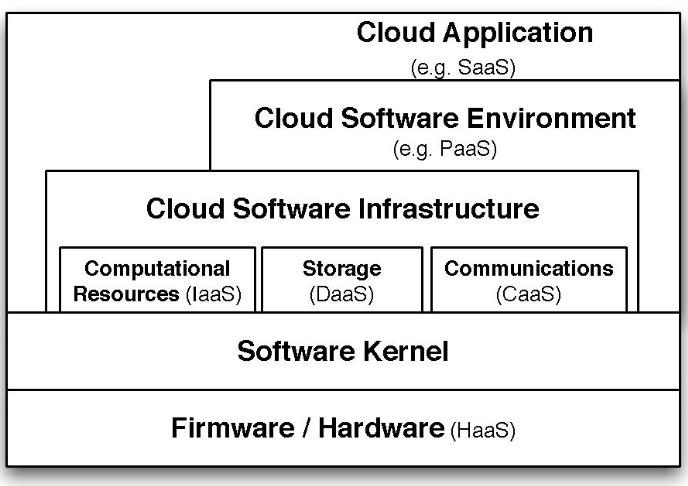
\includegraphics[width=100mm]{images/c_ontology.png}
	 \caption{Ontological Representation of Cloud\label{c_ontology} \cite{ontology}}
       \end{figure}

       In Figure~\ref{c_ontology}, several service models are presented for completeness,
       but within the scope of our research only three service models are relevant,
       namely: \gls{iaas}, \gls{paas} and \gls{saas}. The differences between each
       service model is better understood when it is illustrated by the separation of
       responsibilities between the \gls{csp} and the consumer.

       \begin{figure}[h!]
         \centering
	 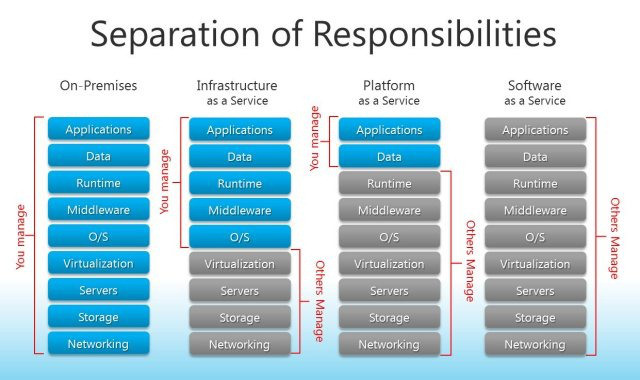
\includegraphics[width=125mm]{images/cloud_sep_of_resp.jpg}
	 \caption{Cloud Services Separation of Responsibilities\label{cloud_sep_of_resp}
           \cite{blewis}}
       \end{figure}

     Figure ~\ref{cloud_sep_of_resp} presents this separation of responsibilities for
     each of these service models.

     % Support Sentence: What is IaaS?
     The \gls{iaas} service model imposes the majority of the responsibilities above the
     virtualization layer to the consumer, whereas the \gls{csp} is responsible for
     providing the physical and virtualization layers. Compared to the other service
     models, it grants greater flexibility to the consumer, using a virtual machine image
     to encapsulate the \emph{complete} executing environment, from the \gls{os} to the
     applications and everything in between. An example of such a service model is
     \emph{Amazon EC2} \cite{AWS}.

     % Support Sentence: What is PaaS?
     \gls{paas} is not as flexible, but it is easier to configure and use. It provides a
     set of abstractions (in the form of an \gls{api} where only the Application layer and
     the Data layer are presented) for the consumer to use to develop applications. The
     \emph{Google App Engine} is a popular example of \gls{paas} \cite{gae_web}.

     % Support Sentence: What is SaaS?
     Finally, \gls{saas} consists of providing an application as a service, where
     everything else is the responsibility of the \gls{csp}. Using this service model the consumer
     accesses a software through the \gls{csp}, and is not required to own a copy, but
     rather leverages its functionalities as services. An example of a \gls{saas} provider
     is \emph{Salesforce}, which offers a multitude of business applications as \gls{saas}
     \cite{salesforce}.

     \subsection{Volunteer Cloud Computing} \label{VCC}
     % Topic Sentence
     Volunteer cloud computing is an emerging paradigm. Conceptually, it is the
     intersection of the public-resource computing paradigm and the cloud computing
     paradigm, it can also be defined as the 5th deployment model of cloud computing. This
     new deployment model consist of constructing a cloud computing infrastructure by
     relying solely on (volunteered) public-resources. It is a fairly recent idea, as it
     is not mentioned in earlier publications such as \cite{taxonomy}, but it is in later
     publications such as \cite{soa_cloud}.

     This paradigm suffers from different challenges compared to the traditional cloud
     computing paradigm \cite{anjomshoa2015taxonomy}, which are similar to the challenges of
     public collaborative systems. Volunteer cloud computing provides a cloud computing
     infrastructure built using volunteered computing resources, whereas public
     collaborative systems provides an infrastructure to perform distributed
     computationally intensive tasks. The dichotomy of their purposes, is what really
     differentiates volunteer cloud computing from public collaborative systems.

     Many different research efforts that attempts to provide this type of infrastructure
     exists with varying degrees of success, and adopting different approaches while
     addressing these challenges. Note that some research efforts, such as
     \cite{cunsolo2010open}, target the full spectrum of service models: \gls{iaas},
     \gls{paas}, and \gls{saas}. Whereas, other focuses on only one service model,
     \gls{iaas} \cite{P2PCS} \cite{chandra2009nebulas}.  Finally, others adopt a
     completely different approach, such as building a transparent infrastructure using
     peer-to-peer interception techniques \cite{mondejar2013cloudsnap}.

     % (0) General Overview
     % (1) Overlay Networks --> Topologies ----> Structured
     %                              |
     %                              -----------> Unstructured
     \section{Peer-to-Peer Computing}
     In this section we present an overview of peer-to-peer computing, we
     introduce the concept of overlay networks, and then detail the differences between
     two types of topologies. Finally, we present a comparative analysis of the topologies
     in the form of a summary table.

     \subsection{Overview}
     % Topic Sentence:
     Peer-to-peer computing has many different characteristics that makes it an
     interesting network primitive for a public environment, such as the Internet, when
     constructing a distributed system.

     A system built using a peer-to-peer structure is referred to as a \emph{peer-to-peer
       system}. Essentially, peer-to-peer systems are defined as a distributed system
     where every node in the system is at the same time, a consumer of the services
     offered by the system and a producer, a server and a client (servent). The cost of
     operations is then amortized and distributed among the participants, because every
     participant in the system assumes the cost of operating their own computers, where
     the aggregate cost of operating the system is the combination of all the costs
     incurred for operating the participants computers. Peer-to-peer systems are generally
     decentralized, removing any single point of failure and resulting in systems that are
     very resilient to the failures of the nodes composing its
     infrastructure. Peer-to-peer systems are also scalable, inasmuch as more nodes are
     available to join the system, theoretically \emph{ad infinitum}. This underlines that
     there are no explicit scalability limitations for this type of system, given that the
     business logic it implements also does not explicitly prevents it (by design).
     % Support Sentence: Division of responsibilities...
     The equality amongst nodes is usually achieved by creating a decentralized network,
     where each node assume equal responsibilities in terms of routing and discovery of
     other nodes within the network. Generally, there are no central servers and all the
     nodes in the system are equal, but practically some system relies on a bootstrapping
     server to ease joining new nodes to the system, which is the case for mobile networks
     \cite{olkkonen2006generic}.

     % Support Sentence: decentralized
     In order to join a system, a node is required to know at least one other node in
     it. Initially, if there are no other nodes in the system, the first node to join will
     become the only node to contact to join this system. Subsequently, the next node that
     wishes to join this system contacts this node, but the third node has the choice to
     contact either the first or the second node, and so on.
     % Support Sentence: after bootstrap
     Once a node has joined the system, it usually has only a partial view of the entire
     underlying network and in order to contact any node not contained within this view,
     it must interact with neighboring nodes for indications on how to proceed.  This
     co-operative location mechanism differs in implementation, but conceptually a node
     requires the assistance of the other nodes, in some ways, to navigate the underlying
     network in its entirety. Consequently, peer-to-peer systems usually construct
     a virtual \emph{overlay network} on top of the physical underlying network, to mitigate
     the complexities inherent to this decentralized architecture \cite{milojicic2002peer}
     \cite{barkai2001peer}.


     \subsection{Overlay Networks}\label{bkg_overlay}
     \emph{Overlay networks} are a fundamental primitive for peer-to-peer systems and can
     be defined as virtual networks superposed on a physical network (the Internet).
     The virtual network represents virtual connections between the different nodes in
     the physical network. It abstracts the underlying physical connections, and exposes
     the logical
     (virtual) connections between the nodes of the system.\\
     
     \begin{figure}[h!]
       \centering
       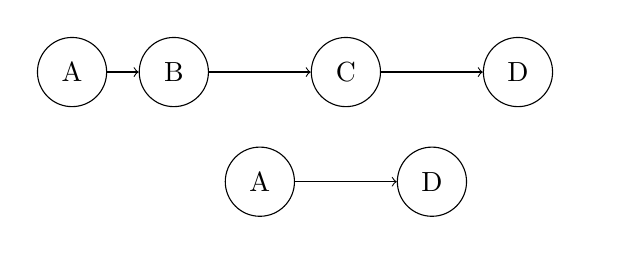
\begin{tikzpicture}[point/.style={circle,inner sep=0pt,minimum
             size=2pt,fill=red}, skip loop/.style={to path={-- ++(0,#1)
               -| (\tikztotarget)}}]

         \matrix[row sep=5mm,column sep=2mm] {

           % First row:
           \node (A) [state] {A};
           & & \node (B) [state] {B};
           & & \node (C) [state] {C};
           & & \node (D) [state] {D};
           \\

           %Second row
           & & &\node (A2) [state] {A};
           & &\node (D2) [state] {D};
           & & &\\ };

         \path  [->]  (A) edge node {} (B);
         \path  [->]  (B) edge node {} (C);
         \path  [->]  (C) edge node {} (D);
         \path  [->]  (A2) edge node {} (D2);
       \end{tikzpicture}
       \caption{Example of Overlay Network Virtual Connections.\label{overlay_fig}}
     \end{figure}

     Figure~\ref{overlay_fig} exemplifies the concept of virtual connections using an
     overlay network. For example: If \textbf{Node A} is connected to \textbf{Node B},
     which is connected to \textbf{Node C}, which is finally connected to \textbf{Node D}
     in the underlying physical network topology. Then, it is possible to express the
     indirect connection between \textbf{Node A} and \textbf{Node D} as a direct virtual
     connection in the virtual overlay network. Not only, overlay networks abstract away
     the details of the underlying network, but also allows nodes to communicate between
     them using this virtual topology.

     Overlay Network topologies are categorized relative to their structure
     \cite{lua2005survey}. In the next sub-sections we present the distinction between a
     \emph{structured overlay network} and a \emph{unstructured overlay network} respectively.

     \subsection{Structured Overlay Network}
     % Topic Sentence:
     What characterizes the structured overlay networks is the fact that they are constructed
     by organizing the peers into a structured graph.

     % Support Sentence: keyspace abstraction
     An abstraction known as \emph{keyspace} is used to organize the participating peers
     into a structure. Each peer is assigned a portion of the keyspace and is responsible
     for locating and indexing keys within it. Partitioning of the keyspace is done according
     to the \emph{keyspace partitioning scheme}, which dictates the structure of the
     resulting network. Some keyspace partitioning schemes can produce a ring topology,
     see \cite{stoica2001chord}; whereas others can produce various different topologies,
     including a tree-based topology, see \cite{jagadish2005baton}

     % Support Sentence: SADQ only
     As a consequence of its static structure, this type of overlay network is not suited
     for complex multi-attribute queries. Because the organization of the keys is
     structured according to a single metric, it only supports single-attribute dominated
     queries. These queries are deterministic, because the attribute for which the queries
     are tested against corresponds to the key and will return upon exact or partial
     match. Ultimately these networks are built around the idea of being able to
     efficiently locate any key within the network.

     % Support Sentence: DHTs
     \gls{dht} is a class of structured overlay networks. It consists of creating an
     overlay network by dividing the keys of an associative array (hash table) among the
     peers, then each peer is responsible for a portion of the associative array. A key in
     this context represents either a node or an entry in the \gls{dht}. To retrieve a
     specific key, a node queries the other nodes to find which one is responsible for
     this key, or finds the node which is responsible for the portion of the associative
     array closest to the key. If neither has the key, the query returns because there are
     no value associated with this key, hence the deterministic nature of \gls{dht}.  Many
     implementation of \gls{dht} exists \cite{sarmady2010survey} \cite{lua2005survey}
     \cite{p2p_collab}.

     Structured overlay networks are constructed to fulfill a specific functionality, such
     as storing data in a distributed fashion, and they are very good at it. But they are
     not as versatile as their unstructured counterparts in terms of applications,
     resistance to failures, and querying abilities \cite{p2p_collab}
     \cite{lua2005survey}.

     \subsection{Unstructured}
     Unstructured Overlay Networks differ with respect to their construction, resulting
     in a unstructured topology, namely a flat or hierarchical random graph. More
     importantly, there are no relations between the topology and the partitioning of the
     keyspace, since technically the keyspace is irrelevant in this context.

     Rather than utilizing a sophisticated partitioning mechanism for the graph, each peer
     connect to another peer in the network, and by performing cyclic exchanges of information
     among them (generally in pair-wise fashion) they update their views of the
     network. Peers only have a local view of the overlay network, but they perform cyclic
     exchanges to achieve local convergence between their views of the network, resulting
     in global convergence of the network topology. As a result of global convergence (or
     network-wide convergence), several self-* properties emerges such as:
     self-configuring, self stabilizing and self-healing properties \cite{pss}
     \cite{birman2007promise}. \emph{Self-configuration} refers to the ability to
     autonomously configure the deployment of a system, or to respond to changes in the
     topology of the composing components \cite{kephart2003vision}
     \cite{berns2009dissecting}. The \emph{self-stabilization} property refers to the
     ability for a system to start in any arbitrary configuration and eventually converge
     to a desired configuration \cite{berns2009dissecting} \cite{dolev2000self}. Whereas,
     the \emph{self-healing} property provides autonomous detection, diagnosis and repair
     of localized problems \cite{kephart2003vision}, but also autonomous component-level
     failure recovery \cite{berns2009dissecting}. Maintaining the overall health of the
     system, can be referred to as the \emph{survivability}, which is the prime objective
     of self-healing components \cite{psaier2011survey} \cite{ghosh2007self}. Given the
     emergence of these properties, this type of overlay network is very robust in highly
     dynamic environments, such as the Internet \cite{birman2007promise}.

     Generally, the routing is done by performing random-walks or flooding the network,
     and consequently querying is not deterministic. Since the structure of the graph, or
     the lack thereof, is not dependent on any particular arrangement of the peers, the
     network supports complex queries because of the arbitrary nature of the routing
     mechanism, which can reinterpret the network accordingly. This is commonly referred
     to as \emph{slicing} and we present it in the following subsection.

     Because of the routing mechanism, location of specific data managed by a peer in
     the network is rather difficult if it has not been replicated on several
     nodes. Replication schemes usually target the most popular data in the network, and
     replicates it across several nodes to ensure availability. Thus, rarely queried data
     is unlikely to be found by queries if it is managed by a single or very small
     collection of peers. Because queries generally have a \gls{ttl}, which
     can be represented in terms of hops or \gls{htl}, after which the query will simply be
     dropped and no result will be returned.

     Examples of unstructured overlay networks are usually based on epidemic protocols, or
     gossip-based protocols \cite{riviere2011gossip}, for which a peer joins the network
     and periodically exchange its local view of the network with another, randomly
     selected, peer.

     For more information on overlay networks, and comparisons on the different types see
     \cite{lua2005survey} and \cite{p2p_collab}.

     \subsection{Slicing}\label{bkg_slice}

     \emph{Slicing} is a primitive in distributed systems, which dictates the querying
     abilities of the underlying network structure. The ability and degree
     to which the system can perform slicing, is relative to the complexity of the queries
     it supports. It can be formulated as the following:
     \begin{quote}
       Given a graph, representing a network of peers, can we partition it according to a
       set of node local-attribute(s).
     \end{quote}
     Several techniques exists to solve this problem as depicted in
     \cite{jelasity2006ordered} and \cite{pasquet2014autonomous}. Techniques varies in
     terms of the type and number of attributes considered, and consists of ordering the
     nodes according to these attributes providing different perspectives of the same
     collection of nodes.

     Based on this definition of the slicing problem, we can now formulate the
     differentiation between \gls{sadq} and \gls{madq}. The distinction arises from the
     ability to query resources, according to the specifications of their attributes,
     whether it support querying a single attribute per query or multiple. Or we can also
     distinguish the two, based on the ability to slice the current network into slices
     (partitions) according to the(se) attribute(s).

     This problem helps deciding which topology of overlay network to use, because it
     illustrate the querying ability provided by the different topologies.

     \clearpage
     \subsection{Comparison}
     We can summarize the advantages and disadvantages of the different types of overlay
     networks according to different characteristics, inspired by \cite{lua2005survey} and
     \cite{p2p_collab}:

     % ----------------------------------------------------------------------%
     {\small\begin{longtabu} to \textwidth {|X[1 , l ] |X[1 , p ] | X[1 , p ]|}\firsthline\hline
     % -----------------These are headings----------------------------------%
     Characteristics  & \textbf{Structured}  & \textbf{Unstructured} \\ \hline
     %
     \endfirsthead
     %
     \multicolumn{3}{c}%
                 {{\bfseries  Continued from previous page}} \\
                 \hline
                 %
     Characteristics  & \textbf{Structured}  & \textbf{Unstructured} \\ \hline\hline
     \endhead
     %
     \hline \multicolumn{3}{|r|}{{Continued on next page}} \\ \hline
     \endfoot
     %
     \hline
     \multicolumn{3}{|r|}{{Concluded}} \\ \hline
     \endlastfoot
     %-----------Headings end---------------------------------
     %--------------------------table body starts-------------------


     \textbf{Construction} &
     % construction --> structured
     Generate abstract keyspace, which is divided among the
     peers. Topology results in a structured graph. &
     % construction --> unstructured
     Peers query a participating node and retrieve information about the network. Repeats
     periodically, results in a flat or hierarchical random graph.\\\hline

     %--------------Construction[END]--------------------------------

     \textbf{Routing} &
     % routing --> structured
     Key-based routing, each node contacts the closest node to the key (according to its
     local view), and then the closest node to this node, and so on until the node
     responsible for the key is reached. &
     % routing --> unstructured
     Perform a random-walk through the network or using flooding techniques. May not
     return a result (query could time-out).\\\hline

     %-------------Routing[END]------------------------------------

     \textbf{Lookup} &
     % lookup --> structured
     Deterministic and has a general time complexity of $O(log n)$, where n is the number
     of keys in the keyspace. &
     % lookup --> unstructured
     Non-deterministic and is generally a best-effort attempt to locate data, popular data
     can be easily located due to replication. No defined boundary in terms of time
     complexity, uses a parameter that represent the TTL, (in seconds or hops). \\\hline

     %-------------Lookup[END]------------------------------------
     \textbf{Join/Leave} &
     % join/leave --> structured
     {\bf Join:} Node contacts a live node and a portion of the keyspace is attributed to
     it, according to its identifier (or key).
     {\bf Leave:} Node leaves, eventually the keys will be remapped to the neighboring
     nodes in the network and all the neighbors table will be updated. &
     % join/leave --> unstructured
     {\bf Join:} Node contact an arbitrary live node and
     exchange information, and repeats periodically forever achieving a dynamic view of
     the network.
     {\bf Leave:} Node leaves, and then since it won't participate in the periodic
     information exchange, it will be discarded from the dynamic view of the network.\\\hline
     %------------Join/Leave[END]--------------------------------

     \textbf{Reliability/Fault-Tolerance} &
     % Reliability/Fault-Tolerance --> Structured
     Resist churn and normal level of node failures. &
     % Reliability/Fault-Tolerance --> Unstructured
     Highly resistant to churn and very high level of node failures. \\\hline

     %------------Fault-Tolerance[END]--------------------------

     \textbf{Slicing} &
     % Slicing --> Structured
     (SADQ) Single-Attribute Dominated Queries &
     % Slicing --> Unstructured
     (MADQ) Multi-Attributes Dominated Queries \\ \lasthline
     %--------------------------table body ends-------------------
     \end{longtabu}}
     %===============================================================

     % (0) General Overview
     % (1) Full Virtualization
     % (2) Light Virtualization
     % (2.1) Containers
     % (2.2) LxC
     % (2.3) Docker

     \section{Virtualization Technologies}\label{bkg_virt}
     In this section we present a general overview of \emph{virtualization}. We
     differentiate between \emph{full virtualization} and \emph{light
       virtualization}. Then, we present what are \emph{containers}, and take a look a two
     different instances of it such as \gls{lxc} and Docker containers.

     % What is Virtualization?
     \subsection{Overview}
     % Topic Sentence:
     Virtualization provides the ability to
     allocate the physical resources needed to accomplish a task prescribed by the software.
     It is \emph{generally} achieved through the decoupling of software from hardware
     \cite{tavangarian2012virtual}.

     The simplest example of virtualization that is used by a majority of \gls{os} are
     processes \cite{chisnall2008definitive}. Processes are isolated into virtual
     environments that exposes the resources as if they are the sole consumer, by
     abstracting the other processes away and effectively decoupling the software from the
     underlying hardware providing the computational resources.

     The concept can be extended to the virtualization of whole \gls{os}s. The
     interactions from the \gls{os} with the physical hardware are done through a software
     abstraction layer, the resulting machine is called a \gls{vm}
     \cite{semnanian2011virtualization}.

     Within the context of distributed systems, one type of virtualization pre-dominantly
     exist, the \emph{full virtualization} or desktop virtualization. Semantically it is
     different from \emph{para-virtualization} and both types shouldn't be conflated. The
     latter requires modification to the guest operating system to comply with the
     interface defined to access the physical hardware. Whereas the former requires no
     such modifications, and the calls from the operating system to the hardware can be
     interpreted directly \cite{tavangarian2012virtual}.

     An emergent type of virtualization technology, known as \emph{light virtualization}
     or operating-system level virtualization, is gaining popularity. It is akin to the
     type virtualization used processes. It is important to draw the differences between
     these two types of virtualizations, in order to understand which is best suited to
     fulfill our requirements. We neglect para-virtualization in the context of this
     thesis since it is not as relevant for our research, as we do not intend to impose
     any modification on the \gls{os}. For more details on the basics of virtualization,
     see \cite{tavangarian2012virtual} \cite{barham2003xen}.

     \subsection{Full Virtualization vs. Light Virtualization}\label{fvvslv}
     % Topic Sentence:
     Several distinctions exist between full virtualization and light virtualization and
     some are advantageous, others are disadvantageous in different contexts.

     % Support Sentence: full virtualization
     \emph{Full virtualization} can be defined as a virtualization technique for which the
     entire hardware is virtualized, providing an abstract computing base, as a software
     layer, on which it is possible to execute a complete \gls{os} without any
     modifications \cite{barham2003xen}.

     % Support Sentence: pros fv
     The use of \gls{vm}, rather than physical machines, offers several key features that
     are desirable in the context of distributed systems. One of these features is the
     ability to clone, which enables the replication of the complete execution environment
     with ease.  Another very desirable feature is the ability to test changes before
     applying them, and the ability to migrate the \gls{vm}s across different hardware,
     which can also be done without much interruption of service. The penultimate feature
     of using \gls{vm}s, as opposed to physical machines, is undoubtedly the ability to
     execute multiple \gls{vm}s in parallel on a single physical machine. It grants the
     ability to have multiple different execution environments without having to dedicate
     a physical machine to each. When applied to servers, this feature is referred to as
     \emph{server consolidation} \cite{tavangarian2012virtual}.

     A \gls{vm} is controlled by an \emph{hypervisor}, which is responsible for
     orchestrating the \gls{vm}s access to the underlying physical resources of the host,
     and it is also known as Virtual Machine Monitor (VMM). It is possible to distinguish
     between two types of hypervisors. The distinction depends on whether or not there is
     an \gls{os} running the hypervisor (Type-2) or if it is directly interfacing with the
     hardware (Type-1) \cite{popek1974formal}.

     VirtualBox \cite{watson2008virtualbox}, is a prime example of Type-2 hypervisor.
     Figure \ref{vm_containers} shows the difference between full virtualization (on the
     left) and light virtualization (on the right). It illustrates how each type of
     virtualization interacts with the hardware through the \gls{os}.

     \begin{figure}[h]
       \centering
       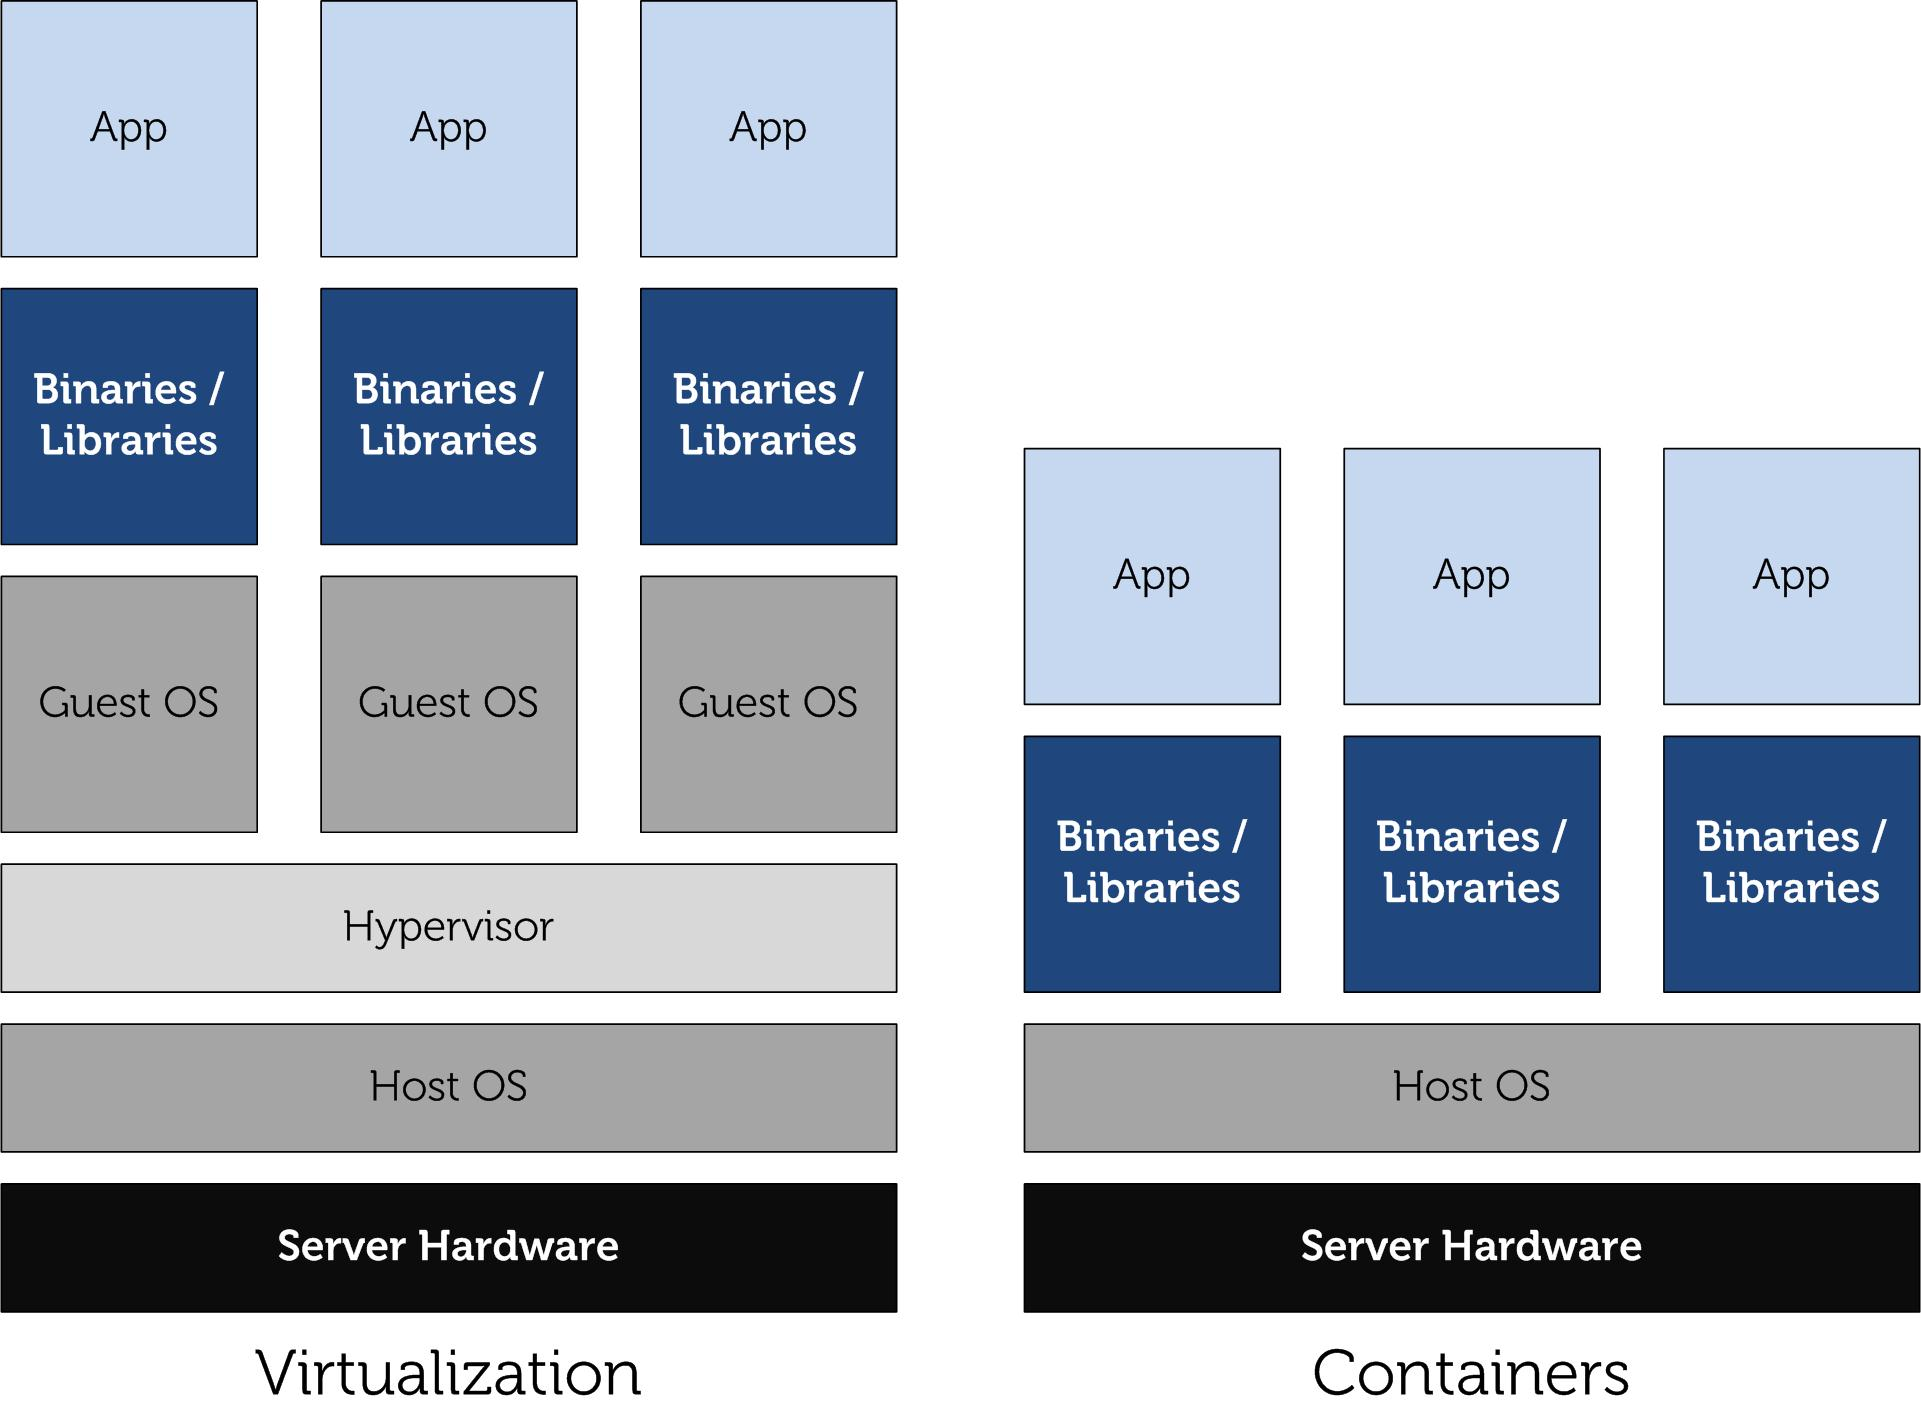
\includegraphics[width=125mm]{images/lxc_vm.jpg}
       \caption{VM vs. Containers\label{vm_containers} \cite{dell}}
     \end{figure}

     % Support Sentence: light virtualization
     \emph{Light virtualization} or operating system-level virtualization, does not
     attempt to execute a complete \gls{os} on top of the current \gls{os}, but rather it
     shares the kernel and the libraries to create fully self-contained environments
     through isolation mechanisms. As a result, light virtulization technologies are
     generally referred to as \emph{containers}.
 
     % Support Sentence: pros lv
     These containers, benefits from similar advantages as their fully virtualized
     counterparts, such as the ability to be cloned, and the ability to run multiple
     instances on a single hardware base. But the feature that sets them apart, is the
     ability to host much more instances on a single machine. This feature is the result
     of using a non-redundant virtualization scheme compared to a full virtualization
     redundant scheme (\gls{os} on top of \gls{os}). This scheme grants a full order of
     magnitude of additional deployment to lightweight virtualization, on identical
     hardware, from 10-100 \gls{vm}s to 100-1000 containers \cite{dell}.

     % Concluding Sentence: (COMPARISON}
     Contrary to full-virtualization, containers do not perform any
     emulation, but rather through namespace isolation re-uses the libraries and kernel of
     the host operating system. This makes it an interesting candidate when using low-end
     hardware, to maximize the hosting capability. But from a security perspective, this
     entails that full-virtualization has a software layer protecting the host \gls{os}
     from the \gls{vm}, namely the hypervisor. Whereas, light virtualization has no such
     layer to protect the host from the container, which has access to the kernel
     interfaces. 

     \subsection{Containers}\label{bkg_cgroup}
     In this subsection we present the technologies that make containers possible in
     Linux. Introduced as a kernel patch \cite{cgroups}, \emph{c-groups} consists of an
     aggregation and partition mechanism for groups of tasks, that contains (within those
     aggregations/partitions) all their children. The central technology behind containers
     in Linux is \emph{c-groups}, or \emph{control-groups}. A c-group allows different
     specialized behaviors to be explicitly defined, by generating a hierarchy of
     groups. The strength of this concept lies in the ability for it to be used with other
     Linux subsystems and to provide additional properties for groups of processes.  One
     example that illustrates the definition of specialized behaviors, consist of pairing
     c-groups with the \emph{cpuset} subsystem to restrict a group of processes to a
     specific \gls{cpu}-core. Through the c-groups technology, and by extending the
     definition of the behaviors of processes in Linux, emerged the container
     technology. We present in the following subsections two different implementations of
     Linux containers, LxC and Docker.

     \subsection{LxC}
     LxC or Linux Containers, is an open-source implementation of the containerization
     technology for Linux. It focuses on providing the tools to facilitate the development
     of system containers in a distribution agnostic fashion \cite{lxc}.

     LxC leverages c-groups partitioning and aggregating capabilities to provide resource
     and namespace isolation without any extra virtualization mechanisms, but rather
     by using the Linux kernel native subsystems. Namespace isolation provides the ability
     to isolate running applications completely from the operating system execution
     environment, albeit not an exclusive feature of LxC. A general example of namespace
     isolation is the \emph{PID namespace}, which provides the means to create sets of
     tasks such that each set is completely independent from one another
     \cite{emelyanov2007pid}. In other words two tasks belonging to different set of
     tasks, can have identical ID without incurring any ambiguity as to which task belongs
     to which set. Resource isolation provides the means (via cgroups) to allocate
     system resources to different groups of tasks.

     Thus, LxC provides capabilities analogous to an operating systems (filesystem, network,
     processes) and dedicated access to the physical resources of its underlying host, in a
     isolated environment in the form of a container \cite{dell}.

     \subsection{Docker}\label{bkg_docker}
     Docker was released on March 2013 and is ever-growing in popularity. It already has
     its own convention: DockerCon \cite{dockercon}, which is endorsed by major
     technological companies such as IBM, Microsoft, Google, and RedHat (to name a few).

     Docker is open-source and provide means to automate deployment of applications within
     containers. It provides a high-level interface to containers, by abstracting the
     intricacies and specificities of the containers into an intuitive and easy to use
     high-level API, providing management, configuration and monitoring capabilities.

     Docker is not a replacement for LxC, rather it is an addition of high-level features,
     on top of the containerization primitives (LxC) of Linux, to interact with
     containers. It implements a custom version of these primitives, largely
     based on the LxC primitives. As does LxC, Docker leverages namespace isolation and
     c-groups to provide isolation to the container, but also uses \emph{union
       file-systems} to provide a lightweight templating system, known as
     images. \emph{Docker Images} are used to specify the operating system environment to
     be instantiated within the container \cite{docker}.

     The union file system is a Unix filesystem service, with which it is possible to
     create virtual filesystems from separate filesystems through branching and
     layering. One of the advantages of this service is the ability to update a filesystem
     by simply applying the difference from the previous versions. In Docker's context,
     this means the ability to update a container by simply uploading the difference (or
     new layer) and applying it, rather than uploading the entire container again \cite{docker}.

     Docker uses a client-server model to communicate between the container (client) and
     the originator/deployer (server), which can reside on a single host or not. Easing
     the workload for the client, because it is possible to offload computationally
     intensive tasks, such as container construction, to more powerful machines while
     conserving lightweight clients \cite{docker}.

     \chapter{Related Work}\label{rel_work}
     In the previous chapter we have presented the background information required to
     understand the following chapters and this information is useful to understand the
     context in which we approach the following related works.

     In this chapter we present the work that relates to our research, notably the two
     most relevant projects: Cloud@Home and Peer-to-Peer Cloud System. But before we
     introduce a framework designed to evaluate collaborative systems \cite{p2p_collab},
     which we use to evaluate the two projects. Finally, we discuss how these
     solutions cater our requirements and what is the scope of these projects.

     \section{Evaluation Framework}\label{rel_EvalFramework}
     The framework proposed by \cite{p2p_collab} aims at formalizing the requirements for
     peer-to-peer collaborative systems. It expresses the functional life-cycle of a
     participant in these systems. Each phases covers a functional requirement, and they
     should be satisfied in a collaborative system to provide a minimally working and
     scalable solution. The 7 key phases of this framework are illustrated in
     Figure~\ref{p2p_collab_fig}.
       \begin{figure}[h]
         \centering
         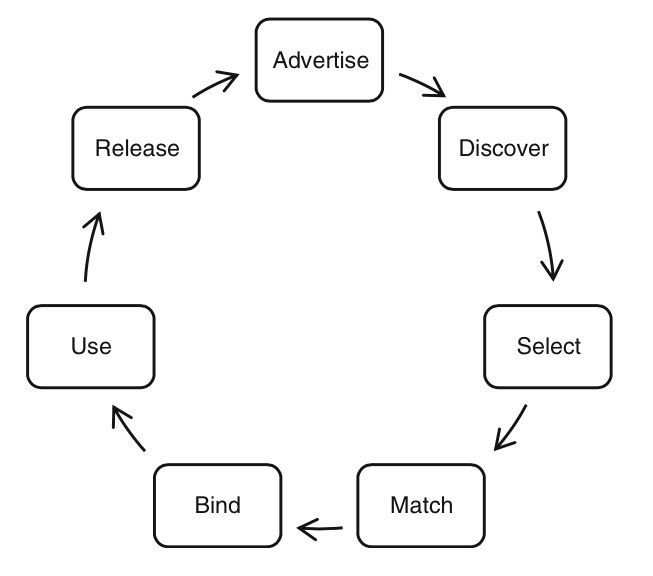
\includegraphics[width=125mm]{images/p2p_collab.jpg}
         \caption{Framework for Peer-to-Peer Resource Collaboration
           Problem \label{p2p_collab_fig} \cite{p2p_collab}}
       \end{figure}

     \begin{enumerate}
     \item \textbf{Advertise}: Each node advertises its resources and their capabilities
       using formal specifications over a set of attributes.
     \item \textbf{Discover}: A mechanism to discover and keep track of the
       useful specification advertisements from the other participating nodes. This
       enables to accelerate the querying mechanisms but also to preserve inter-resource
       relationship information.
     \item \textbf{Select}: A mechanism for a user to select a group(s) of resources, that
       satisfies a formal specification of his requirements defined in a query containing
       the attributes and ranges of acceptable values for these attributes.
     \item \textbf{Match}: A mechanism to be able to formally
       specify inter-resource relationship requirements and to ensure that
       the nodes selected satisfies the resource and application constraints, in the query.
     \item \textbf{Bind}: Provides a binding mechanism between the resources
       and the applications, preventing two applications from selecting the
       same resources. But also to cope with the dynamic nature of p2p,
       since a node may not be available at the time of use but was at the
       time of selection.
     \item \textbf{Use}: Utilize the best subset of available resources,
       from the resources acquired, to execute the application (and all its
       tasks) while respecting the utilization agreement between the application and the
       resources.
     \item \textbf{Release}: Provides a mechanism allowing to release (some)
       resources in relation to the application demand, and/or the
       contractual binding (if time-sensitive). This mechanism can also
       provide the means to partially release a resource and to enable that resource to
       collaborate with other applications simultaneously.
     \end{enumerate}

     Thus, if one were to implement each one of these functional requirements into a
     separate module, then the resulting system would be modular and would ensure proper
     collaborative behavior. For more details on this framework and for an evaluation
     conducted on different peer-to-peer collaborative systems using this framework, see
     \cite{p2p_collab} \cite{bandara2012evaluation}.

     For our purposes this framework acts as a checklist to identify how each of the
     functional requirements inherent to collaborative systems are implemented in the
     following two projects. Ultimately, we will use it in further chapters to assess the
     fulfillment of these functional requirements in \emph{our} own architecture.

     \section{Cloud@Home}
     Cloud@Home is a new paradigm which spawned at the intersection of two existing
     paradigms: the \emph{public-resource computing paradigm} and the \emph{cloud
       computing paradigm}. It is one of the earliest attempt to create a \emph{volunteer
       cloud computing infrastructure}. Over several publications, the authors have
     analyzed extensively the challenges relating to volunteer cloud computing,
     \cite{cunsolo2009volunteer} \cite{aversa2011cloudperf} \cite{aversa2011cloud}
     \cite{cunsolo2010applying} \cite{cunsolo2010volunteer} \cite{distefano2010taxonomic}
     \cite{cathome6} \cite{cunsolo2010cloud} \cite{cathome9} \cite{cathome11}
     \cite{distefano2011qos}.

     Their vision is to offer a full-fledged cloud computing infrastructure constructed
     from volunteered. Full-fledged, in this context, means that they want to provide the
     following service models: \gls{iaas}, \gls{paas} and \gls{saas}. The Cloud@Home
     system aims at offering performances and \gls{qos}\ similar to major \gls{csp}.

     To fulfill some the performance requirements, the authors focused on
     \emph{interoperability} between \gls{csp}, providing a user with the ability to
     contract resources from commercial \gls{csp}s, given that the volunteered resources
     available are insufficient or inadequate. Whereas to fulfill the \gls{qos}
     requirements, they require that both parties negotiate the expected or desired
     \gls{qos} contained in a \gls{sla}, created by the resource consumer. In other words,
     the consumers provide their intended terms of use, relative to the resources, and the
     providers can decide whether or not they accept the terms of use. In case of
     disagreement with the \gls{sla} and the \gls{qos} it contains, the negotiation
     process is aborted. For more details pertaining to the \gls{qos} and \gls{sla} in the
     context of this system, see \cite{distefano2011qos}.

     Contrary to the \gls{csp}, because Cloud@Home uses volunteered resources, the authors
     were obligated to ponder on how to entice people to contribute their resources to
     this infrastructure. They have devised an incentive-based business model, that offers
     financial restitution to the users for their contributions. This model proposes to
     recycle current idling resources into a utility that can be sold, with respect to
     the quality and capabilities of these resources.

     In the following subsections we will present and discuss the architecture proposed for
     this solution, and discuss its conformance to our requirements and the
     evaluation framework.

     \subsection{Architecture}\label{rel_cat_arch}
     The Coud@Home system architecture, shown in Figure~\ref{cat_arch}, is composed of
     three layers: the \emph{Frontend Layer}, the \emph{Virtual Layer} and the
     \emph{Physical Layer}. The functional representation of the infrastructure, shown in
     Figure~\ref{cat_arch_fr} is divided into the \emph{Management Subsystem} and the
     \emph{Resource Subsystem}.

     \begin{figure}
       \begin{subfigure}{.5\textwidth}
         \centering
         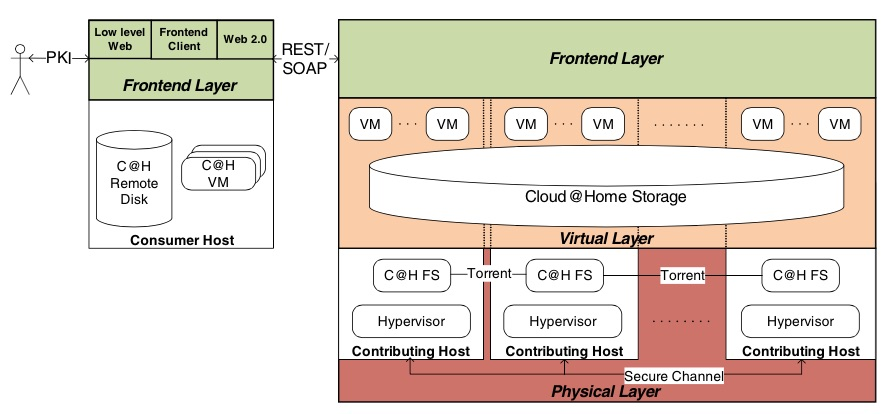
\includegraphics[width=75mm,height=50mm]{images/cathome_arch.jpg}
         \caption{Overview \cite{cathome}}
         \label{cat_arch}
       \end{subfigure}
       \begin{subfigure}{.5\textwidth}
         \centering
         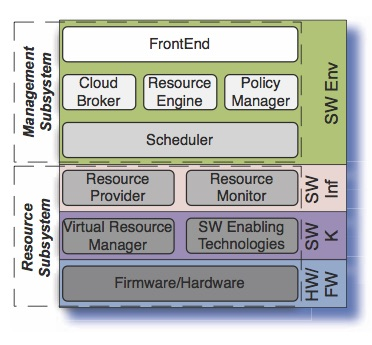
\includegraphics[width=50mm,height=50mm]{images/cathome_fr.jpg}
         \caption{Functional Representation \cite{cathome9}}
         \label{cat_arch_fr}
       \end{subfigure}
       \caption{Cloud@Home Architecture}
       \label{fig:test}
     \end{figure}

     Starting by the architectural overview, the first layer or \emph{Frontend Layer}, is
     responsible for providing a high-level service-oriented point of view of the
     underlying infrastructure. \emph{Consumer Host, in this context, represents a consumer
       of the cloud service provider and not a consumer of the application deployed in the
       cloud.} The relation between the Consumer Host and this layer is based on a
     client-server relationship, providing a centralized point of access to the
     infrastructure.

     The \emph{Virtual Layer} provides a homogeneous perspective of a set of heterogeneous
     resources, by means of virtualization. Because it uses virtualization, it is possible to
     completely abstract the underlying hardware specificities of the different
     contributors resources and to exploit them in a platform-agnostic way. This layer is
     further divided into two services: the \emph{Execution Service} and the \emph{Storage
       Service}. The former enables the consumers to host and execute \gls{vm}s, according
     to their needs, providing a similar service as the Infrastructure-as-a-Service model
     provides. Contributors are then assigned an arbitrary virtual machine to host, or multiple
     \gls{vm}s to host, relative to their intended contributions. Whereas the latter
     provides a distributed storage facility by implementing a distributed file system
     such as \cite{gfs}. Consumers can then mount locally a remote disk that corresponds to a
     portion of the distributed file system. As for contributors, they host an arbitrary
     portion of this distributed file system, relative to the amount of disk space they wish to
     contribute, providing a unified view of the entire distributed file system to the
     consumers.

     The \emph{Physical Layer} is responsible for connecting the contributing resources
     together and providing means for communication. Negotiations for the resources
     between the contributors and the consumers are performed at this layer. The
     negotiation process consists of a request for resources emitted by the consumer,
     followed by an attempt to match the parameters of this request with the parameters of
     the volunteered resources available. The authors specified several mechanisms to ensure and
     negotiate the Quality of Service and Service-Level Agreements between consumers and
     contributors (or \gls{csp}) \cite{aversa2011cloudperf}\cite{aversa2011cloud}.

     The \emph{Management Subsystem} translates the user's requests into multiple
     sub-requests. Whether it is possible for the requests to be satisfied, using
     volunteer resources or their commercial resources, depends on the \gls{qos} specified
     by the user and if it is compatible with the resources available. These request(s)
     are passed on to the Resource Subsystem which binds and matches the resources to the
     user from which the(se) request(s) originated. The Management Subsystem is
     centralized in order to manage the infrastructure, and to manage the \gls{qos} and
     the \gls{sla} of all the resources, but also to provide dynamic provisioning. The
     authors claim that it is the only way to aggregate the global information of the
     infrastructure and to provide a reliable perspective of it \cite{cunsolo2010open}.

     Finally, the authors proposed a middleware that implements the ideas from the
     architectural overview and the functional representation, covering the different
     goals posed by the Cloud@Home paradigm. Figure~\ref{cathome_infra} showcases the
     deployment middleware of the Cloud@Home infrastructure.

     \begin{figure}[h]
       \centering
       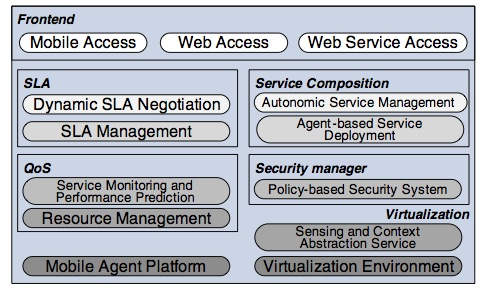
\includegraphics[width=90mm]{images/cathome_infra.jpg}
       \caption{Cloud@Home Infrastructure Middleware\label{cathome_infra} \cite{aversa2011cloud}}
     \end{figure}

     In this overview, we have presented a simplification of the functionalities of the
     two subsystems for more details consult \cite{cunsolo2010open}. For more details on
     the different layers composing its architecture consult \cite{aversa2011cloud}, and
     finally, for more information on the middleware consult \cite{cunsolo2010applying}.

     \subsection{Evaluation}
     In this subsection we evaluate the system according to the evaluation framework that
     we have introduce in Section~\ref{rel_EvalFramework}. Then, we evaluate the system
     against the functional requirements that we have identified in ~\ref{int_req}.

     \subsubsection{Evaluation Framework}
     % Topic Sentence:
     We use the evaluation framework from Section~\ref{rel_EvalFramework} to identify any
     functional deficiencies present in this system relating to the essential requirements
     of peer-to-peer collaborative systems. These functional requirements need not to be
     implemented as being mutually exclusive, and a subset of these requirements can be
     combined into a single module.

     % Support Sentence: Advertise, Discover, and Select...
     As a matter of fact, such is the case for the first three phases. \textbf{Advertise},
     \textbf{Discover}, and \textbf{Select} are accomplished by the Management Subsystem.
     They are grouped together to provide the ability to a user to enroll and
     advertise its resources, or to a consumer to find resources that are available
     according to their needs.

     % Support Sentence: Match, Bind, Use, and Release
     It is also the case for the remaining phases, \textbf{Match}, \textbf{Bind},
     \textbf{Use}, and \textbf{Release}, all being accomplished by the Resource
     Subsystem. It provides the ability, given a request, to match the resources which
     satisfies the request, then to allocate the resources to the consumer in order to use
     them. Upon using the resources, it is possible to release or to deallocate the
     resources when the consumer no longer requires them. As a consequence, it provides
     \emph{dynamic membership} capabilities to the resources, permitting to add or
     remove resources according to the \gls{sla} or the current workload.

     % Concluding Sentence:
     Essentially all the functional requirements present in the evaluation framework are
     fulfilled in one way or another, directly or indirectly. As a consequence, this
     project is appropriately devised to address the essential functional requirements of
     a peer-to-peer collaborative system.

     \subsubsection{Functional Requirements}
     % Topic Sentence:
     We now evaluate how this system addresses our functional requirements, as presented in
     Section~\ref{int_req}, enlightening us on how it could address the research questions
     presented in this thesis.

     % Support Sentence: Req 1
     Starting with the first requirement, which entails the use of commodity hardware to
     form the infrastructure on which it is possible to deploy multiple applications. By
     leveraging public-resources as part of the resources available to deploy an
     application, and by supporting the deployment of multiple applications
     simultaneously, we can assess that this requirement is completely satisfied.

     As for the second requirement, which states that no third-party should be introduced
     to provide any services, in order to maintain self-containment of the system. We can
     only assess partial satisfaction of this requirement, because it is possible using
     this system to rely exclusively on contributed resources, and not contract resources
     from any commercial \gls{csp}. But in order to use this infrastructure, both
     consumers and contributors are required to interface with the Management Subsystem,
     and to an extent this is a third-party in relation to the consumer and contributor.

     The third requirement, states that the system should be resistant to resources
     failing and should not introduce any single point of failures, for security
     purposes. The Cloud@Home system focuses on creating a middleware that is lightweight,
     and this middleware is built around the concept of service migrations. Upon failure
     of any resources, the system can swiftly migrate the workload to any other available
     resources, resulting in an infrastructure optimized for lightweight services and
     failure-resistant. Unfortunately, this system is built around the concept that a
     central server is required to manage its infrastructure, as stated previously
     Section~\ref{rel_cat_arch}. Although, some fault-tolerant mechanisms are put in place
     to mitigate this single point of failure, including redundant servers, and the
     authors claim it is sufficient. Further tests and benchmarks are required to
     corroborate their claims, in a realistic environment, and to satisfy the this
     requirement.

     The fourth requirement, states that no special equipment should be required to access
     and participate in this system, but rather encourage resource
     recycling. Consequently, it implies, as a sub-requirement, that the memory footprint
     should be small enough to enable legacy equipment are able to participate in this
     system. Because this system relies on full virtulization technology, it forces the
     contributing peers to host \gls{vm}s in order to contribute a computational
     resource. Limited resources are expected to be consumers rather than contributors,
     except in very specific cases where the application lends itself to it. Such cases
     are when the limited resources are used for sensorial inputs, such geo-location,
     accelerometers, barometers, and other various sensors that could be used as a
     stream of information available to any applications in the cloud. These stream of
     informations are analogous to nodes in a sensor network. It is clear
     to which extent the memory footprint is small in the context of the proposed
     \gls{iaas} model, but not so much in the context of the other service
     models. Cloud@Home offers \gls{paas} capabilities by using their \emph{SLA Engine},
     ensuring the availability and capacity of the resources, and \emph{CHASE (Cloud@Home
       Autonomic Service Engine}, which determines the optimal configuration parameters
     for the service application using the current configuration of the cloud. Given that
     this processing occurs at the centralized server, it shouldn't incur a large memory
     footprint on the contributing resources. But the contributing resources are still
     required to host \gls{vm}s. This requirement is not completely satisfied.

     The fifth and final requirement, states that the system should provide dynamic
     membership capabilities to all applications, which means that for every application
     it should provide means to scale according to the fluctuations in the workload. The
     Management Subsystem enforces the resources \gls{sla} and guarantees the \gls{qos}, and
     consequently it will preempt the necessary resources to ensure that they are
     only used to the extent prescribed in the \gls{sla}. This system supports
     dynamic membership, and consequently provides scalability to the applications
     deployed, resulting in the satisfaction of this requirement.

     Out of the five requirements: one remains unsatisfied, three are partially satisfied
     and one is completely satisfied. We can conclude that this system does not address
     our research question sufficiently for it to be considered a viable solution, and
     thus we must find a more adequate solution or create one.

     \section{Peer-to-Peer Cloud System}
     % Topic Sentence:
     The \gls{p2pcs}, was developed as part of a doctoral thesis \cite{P2PCS}, and
     proposes a slightly different approach to volunteer cloud computing than the previous
     system. One of the defining characteristic of this system is the fully decentralized
     structure connecting the different peers, constructed using epidemic and gossip-based
     protocols.

     The authors propose an infrastructure with no centralized server(s) to manage the
     resources, conversely to the Cloud@Home system. Rather each node interact directly
     with the other nodes when performing any system operations. Consequently, the
     consumer nodes interacts directly with the (potential) contributing nodes in order to
     select the fittest candidates to host the application. Fitness of a candidate is
     evaluated using the response of a specially defined query, which contains the desired
     criteria for candidate resources (e.g., 10 nodes with at least 8 gigabytes of
     RAM...). The collection of nodes that fulfills these criteria are selected and they
     form a \emph{Slice}. This slicing mechanism is an \emph{attempt} at solving the
     slicing problem presented in Section~\ref{bkg_slice}. The consumer would communicate
     with this slice, or pool of nodes, via an \gls{api} that is similar to what current
     \gls{iaas} provider (Amazon EC2 or S3) uses. Using this \gls{api}, the consumer is
     able to instruct the contributing nodes on when to start or stop \gls{vm}s according
     to the application requirements. The authors present this system as a peer-to-peer
     cloud computing architecture focused on providing only one service model, the
     \gls{iaas}.

     In the following subsections we present the architecture of the system, and proceed
     to evaluate the system against the evaluation framework and our functional
     requirements, as we did for the previous system.

     \subsection{Architecture}
     % Topic Sentence:
     The architecture is divided into 3 functional components, although the authors did
     not explicitly use nomenclature to distinguish between correlated components, we do.

     \begin{figure}[h]
       \centering
       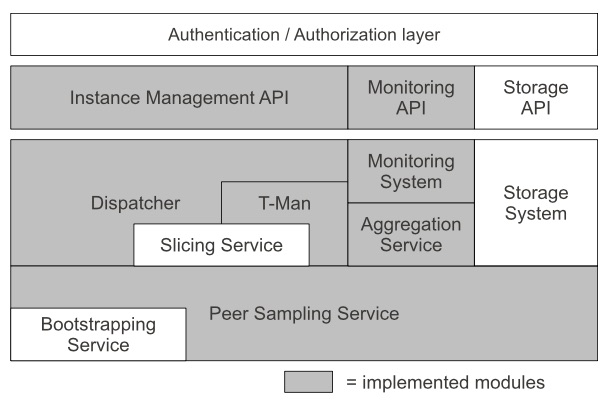
\includegraphics[width=125mm]{images/p2pcs_arch.jpg}
       \caption{Peer-to-Peer Cloud System Architecture \label{p2pcs_arch} \cite{p2p_collab}}
     \end{figure}

     Figure~\ref{p2pcs_arch} presents the different components of this system. The authors
     distinguished between what has been implemented (in gray) and what has been left as
     future work (in white).

     Using a top-down approach, we present the first component, representing the point of
     access to the system. The \emph{Authentication/Authorization layer} is where a user
     (contributor/consumer) is required to identify themselves in order to access the
     system.

     The second component represents the principal access point to the cloud for the
     consumers, it is named the \emph{\gls{api} layer}, It is composed of three
     sub-components providing different capabilities through various interfaces. The
     \emph{Instance Management API} sub-component provides an interface that circumscribes the
     possible interactions between the consumer and the contributing nodes, with respect
     to the \gls{vm} instances. Whereas, the \emph{Monitoring API} sub-component provides a
     visual representation of the slice topology, and the \emph{Storage API} sub-component provides the
     means to configure the distributed storage system for the current slice.

     The third component represents the \emph{Networking layer}. This component is
     composed of three sub-components, which in turns are composed of three or less
     components.

     The first component of the Networking layer is composed of two services, which are
     the \emph{Bootstrapping Service} and the \emph{Peer Sampling Service}. As it name
     implies, the former provides the bootstrapping mechanism for a node to join this
     system. Whereas the latter, provides a list of peers in the network to exchange
     messages with. The creation and maintenance of the list is accomplished by creating
     and maintaining an overlay network over all the peers in the system. This overlay
     network is created using a simple gossip-based protocol as presented in
     \cite{pss}.

     The second component of the Networking layer is composed of three sub-components,
     which are the \emph{Dispatcher}, the \emph{T-Man} and the \emph{Slicing Service}. The
     \emph{Dispatcher} sub-component is responsible for the translation of the commands
     issued through the various interfaces by the consumer into commands that are
     compliant with the gossip-based protocol(s) used in this system. The following
     sub-component, is \emph{T-Man}, a gossip-based protocol providing the ability to
     create and manage structured overlay networks, using various topologies
     \cite{jelasity2009t}. Whereas the last sub-component, the \emph{Slicing Service},
     provides the slicing capabilities for this system. This entails, as presented in
     Section~\ref{bkg_slice}, ordering the nodes according to node-local attributes, then
     dividing the nodes according to various thresholds. Previously, we have presented the
     slicing capabilities of this system as being an attempt to solve the \emph{slicing
       problem} because of how it is implemented. The (current) implementation enables the
     creation of slices using only one metric, which is completely independent of any
     node-local attribute, consisting of the number of nodes a consumer wishes to
     contract.

     The last component of the Networking layer is also composed of three sub-components,
     the \emph{Monitoring System}, the \emph{Aggregation Service} and the \emph{Storage
       System}. Through the corresponding \gls{api}, the \emph{Monitoring System} provides
     to the consumer access to global system information collected and computed by the
     \emph{Aggregation Service}. The \emph{Aggregation Service} provides system-wide
     parameters to the peers of the system. These parameters are computed by aggregating
     the various local parameters from each peer, through local message exchange among
     peers. To accomplish this in a decentralized and dynamic environment, this service
     uses a \emph{push-pull} gossip-based protocol, as presented in
     \cite{jelasity2005gossip}. The last sub-component is the \emph{Storage System}. It
     provides the distributed storage capabilities of this system and it is accessed
     through its \emph{Storage \gls{api}}.

     From this overview of the architecture of this system, we can observe that gossip-based
     protocols are prevalent, which is \emph{the} defining characteristic of this system. These
     protocols are praised for their ability to strive in highly dynamic and volatile
     environments, and a considerable amount of literature has been published on the
     subject. For a discussion on the limitations inherent to these protocols,
     and its strengths see \cite{birman2007promise}. For a more introductory approach to
     gossip-based and epidemic protocols in the context of distributed systems see
     \cite{jelasitygossip}.


     \subsection{Evaluation}
     In this subsection we evaluate this system against the evaluation
     framework, as presented in Section~\ref{rel_EvalFramework}, then against our
     requirements, as presented in Section~\ref{int_req}.

     \subsubsection{Evaluation Framework}
     % Topic Sentence:
     Again, we rely on the evaluation framework to identify any functional deficiencies
     present in this system, with respect to the essential requirements of peer-to-peer
     collaborative systems. As stated previously, the requirements of this framework can
     be implemented alongside other functional requirements as part of a single module.

     The first two phases, \textbf{Advertise} and \textbf{Discover}, are coupled together
     within the \emph{Peer Sampling Service}. But they are not exhaustively
     implemented. We underline the fact that the system provides no mechanism to advertise
     the resources, a node has to offer, to the network explicitly. Either by using formal
     specifications, as proposed in \cite{p2p_collab}, or using any other
     strategies. Rather, this service presents a node to the other nodes using a
     gossip-based protocol. We deem these functional requirements to be partially
     fulfilled, because it is desirable to be able to advertise and discover resources
     based on the capabilities.

     The \textbf{Select} phase, is accomplished by the \emph{Slicing Service}. The authors
     designed this system to use a gossip-based protocol to automatically partition the
     network into slices according to a metric \cite{jelasity2006ordered}, but was this
     not implemented and slices are created based on the number of nodes desired. Thus, we
     deem this functional requirement to be partially fulfilled, because it is not
     possible to select the resources according to their capabilities.

     The \textbf{Match} phase is suspected to be realized by the \emph{Slicing Service},
     by furthering the specification of the select query. But the limitations of the
     gossip-based protocol used are not clear. Because the slicing mechanism proposed by
     the authors is based on a utility function that describes the usefulness of a node
     with respect to the other nodes, using node-local attributes; and to introduce
     additional dimensions to perform multi-dimensional slicing using a utility function
     is not the best approach since it introduces all sorts of statistical distortions
     \cite{pasquet2014autonomous}. Thus, we also deem this functional requirement to be
     partially fulfilled, because support for multi-dimensional slicing is not explicitly
     provided.

     \textbf{Bind}, the fifth phase, is achieved using the \emph{T-Man} gossip-based
     protocol. This protocol is used to create a ring overlay of all the peers contained
     in a specific slice, 1 ring per slice, resulting in mutually exclusive slices. There
     are no indications on how to cope with concurrent attempts to bind overlapping sets
     of resources, given that these resources satisfies multiple selection queries. This
     is due to the fact that the slicing mechanism uses a single
     metric, namely the number of requested nodes. Then instances of the concurrent binding
     problem would only occur in very a specific case. Manifesting itself in the
     form of two or more concurrent requests, for which the total requested number of nodes
     combined exceeds the total number of available nodes, but the number of nodes
     per request is inferior to the total available nodes. The problem then becomes,
     which application is entitled to have their request fulfilled? Because no a-priori
     ranking mechanism (or reputation mechanism) to decide which consumer should be
     favored is provided, the behavior of the system in response to this characterization of the
     problem is undefined. Again, we deem this functional requirement to be only partially
     fulfilled, because of the lack of concurrent binding requests support.

     The sixth phase, referred to as the \textbf{Use} phase, is satisfied by the
     \emph{Dispatcher}. It translates the higher-lever API requests into the appropriate
     low-level gossip protocol commands sent to the other nodes, resulting in the
     utilization of the resources. This functional requirement is completely fulfilled,
     because this system provide the ability to use the selected resources.

     The last phase, \textbf{Release}, can be accomplished by the \emph{Instance
       Management API}, granting the ability to the consumer to control the \gls{vm}s
     instances it was assigned. The automation of this phase would be the result of the
     co-operation between the \emph{Monitoring System} and the \emph{Aggregation Service}.
     collecting global information about the system, such as the current load in a
     slice, and acting on these results by preempting the necessary amount of
     resources. This functional requirement is also completely fulfilled, because using
     the \emph{Instance Management API} in concert with the \emph{Monitoring System} and
     \emph{Aggregation Service} provides the ability to release resources when they are no
     longer required.

     According to the evaluation framework, this architecture exhibits \emph{some} of the
     characteristics that are essential in a peer-to-peer collaborative system. Only
     \emph{two} out of the \emph{seven} functional requirements are completely fulfilled,
     and \emph{five} are only partially fulfilled either conceptually or because of the
     lack implementation. Nonetheless, this system presents a solid foundation that could
     be extended to meet all the requirements, because there are no apparent design decision
     that would explicitly prevent it.

     \subsubsection{Functional Requirements}
     We evaluate this system against our functional requirements, defined in
     Section~\ref{int_req}.

     The first requirement, states that it should be possible for the infrastructure to be
     constructed using only commodity hardware and that it should host multiple
     applications at once. By relying solely on user contributed resources and by
     providing the ability, to the consumers, to create mutually exclusive slices for their
     applications, this requirement is deemed to be completely fulfilled.

     As for the subsequent requirement, which states that every services should be
     provided by the contributing resources, not 3rd-parties, we can conclude that it is
     fulfilled. We arrive at this conclusion by observing that the proposed system relies
     solely on contributed resources and thus it does not introduce any 3rd-parties.

     The following requirement states that system should not introduce any single point of
     failure, and the system should be (somewhat) resistant to ubiquitous failures.  As a
     consequence of being fully decentralized this architecture does not introduce any
     single point of failure. Using gossip-based protocols to create and maintain the
     overlays it is able to cope with a very dynamic networking environment. Failures or
     node leaving/joining the network, are well supported by these protocols, thus we deem
     this functional requirement to be fulfilled \cite{p2p_collab}.

     The following requirement states that no special or dedicated hardware should be
     necessary to participate in this system, and consequently that memory footprint
     should be as low as possible as to enable a wider range of (weaker or lower-end)
     resources to participate. Nothing requires from a participant to acquire any special
     or dedicated equipment to participate in the system. For the \gls{iaas} model it is
     required to use full virtualization technologies, increasing the memory footprint,
     and it is not clear as how it would fare on lower-end resources. Thus we cannot deem
     this functional requirement to completely fulfilled, because it uses
     full-virtualization technologies and the authors have not shown the memory footprint
     to be small.

     The last requirement states that the system should be able to provide scalability to
     the applications deployed, and consequently provide dynamic membership capabilities.
     As stated previously, the use of gossip-based protocols facilitate the support for
     dynamic membership capabilities because of their resistance to failures and
     arrival/departure of nodes. Consequently, this functional requirement is deemed to be
     fulfilled.

     Ultimately, this system fulfills \emph{four} out of the \emph{five} functional
     requirements explicitly, making it almost a viable solution, but not quite. We put
     the emphasis on the fact that the system adopts sensible approach to solve our
     problem, but the limitations present dissipates any hopes of redeeming it. To back
     these claims, we want to outline the fact that a lot of the problems of providing a
     distributed computing platform are simply relayed to the end-user when adopting a
     \gls{iaas} model. Because it reverts the responsibilities to mitigate the problems,
     back to the user, in the form of (proper) configuration of the \gls{vm} instances
     required for any applications. Thus, we think that this system does not, and could
     not without substantial modifications, provide a \gls{paas} computing platform or a
     system capable of addressing our research requirements.

     \section{Discussion}
     % Topic Sentence:
     In this section, we discuss the various details and implications of both projects, and
     provide a reflection on what they accomplish from a high-level overview.

     The Cloud@Home system offers a decent solution to the volunteer cloud computing
     paradigm but also with respect to the functional requirements of peer-to-peer
     collaborative systems. This solution trades off full decentralization and the
     capacity to leverage lower-end resources for augmentation of performance and
     \gls{qos}. It introduces possible third-parties, in order to provide these
     performance and \gls{qos} guarantees, and thus it breaks our perspective of being
     fully self-contained with respect to the consumers and contributors. It aims at
     providing a business model to transform current computing resources into a utility
     that can be monetized.

     In contrast, \gls{p2pcs} provides an architecture that can transform a group of
     computing resources into a application deployment platform, corresponding to the
     \gls{iaas} model. This system provides the ability to leverage resources using
     full-virtualization, but it does not provide a business model to justify the
     viability of the infrastructure, or to provide any incentive to entice possible
     contributors. Like many open-source and community-driven project it anticipates a
     self-policing behavior from the community. The \gls{api} proposed to interface with
     the resources is analogous to traditional \gls{iaas} \gls{api}s. The strength of this
     system lies in the adoption of gossip-based protocols to accomplish the underlying
     network creation and maintenance. Consequently, by using these protocols it mitigates
     a lot of the complexities and difficulties of operating a distributed system over
     unreliable network infrastructure, such as the Internet.

     Both of these projects offer interesting architectures supporting a multitude of
     desirable features for volunteer cloud computing and public-resource computing, but
     from our perspective some key features are still missing. Notably the ability to
     leverage a collection of commodity devices to provide a multi-application computing
     platform akin to a \gls{paas} model, by limiting the memory footprint. The
     \gls{paas}e model has different concerns compared to the \gls{iaas} model, with
     respect to security and isolation. The latter uses \gls{vm}s, to isolate the
     contributing environment from the hosting environment. And it is not clear how this
     could be accomplished in either projects without resorting to \gls{vm}s. Consequently,
     providing a \gls{paas} model, using the contributed resources rather than
     leveraging a commercial service provider, remains unresolved for \gls{p2pcs} and
     problematic for Cloud@Home when using lower-end resources.

     Ultimately, due to the deficiencies outlined, we express the need of creating an
     architecture based on the observations we made while evaluating these projects.
     \\
     
     \begin{table}
     \begin{tabular}{l*{3}{c}}
       & Cloud@Home & P2PCS & Our Architecture \\ 
       \hline
       \textbf{Evaluation Framework}\\
       \hline
       Advertise & + & + & ++ \\
       Discover & + & + & + \\
       Select & + & + & ++ \\
       Match & + & + & + \\
       Bind & + & + & + \\
       Use & + & ++ & ++ \\
       Release & + & ++ & + \\
       \hline
       \hline
       \textbf{Functional Requirements}\\
       \hline
       Requirement 1 & ++ & ++ & ++ \\
       Requirement 2 & + & ++ & ++ \\
       Requirement 3 & - & ++ & ++ \\
       Requirement 4 & ++ & ++ & ++ \\
       Sub-Requirement 4.1 & + & + & + \\
       Requirement 5 & ++ & ++ & ++ \\
       \hline
       \hline
       \textbf{Legend:} &&&\\
       & ++ = completely fulfilled &&\\
       & + = partially fulfilled &&\\
       & - = not fulfilled &&\\
     \end{tabular}
     \caption{Summary of the Solutions and the Requirements}
     \end{table}


     \chapter{Architecture}\label{arch_chap}
     In this chapter we present the architecture we have proposed, and illustrate the
     different decisions that influenced our design. We designed this architecture based
     on the observations made in the related works, and our design takes into account our
     requirements, as presented in Section~\ref{int_req}, and the essential functional
     requirements for peer-to-peer collaborative systems, as presented in Section
     ~\ref{rel_EvalFramework}.

     The first section provides a high-level perspective of the architecture, whereas the
     subsequent sections present and express the design rational behind each layer. We
     then present an exploration of the various components of this architecture and their
     interactions. We conclude with a discussion of the requirements that were addressed
     by designing this architecture.

     \section{Overview}\label{arch_over}
     We used a multi-tiered approach for the architecture, similar to Cloud@Home and
     \gls{p2pcs}, because it provides high modularity and loose coupling of the concerns
     addressed by each tier.
     % Figure
     \begin{figure}[h]
       \centering
       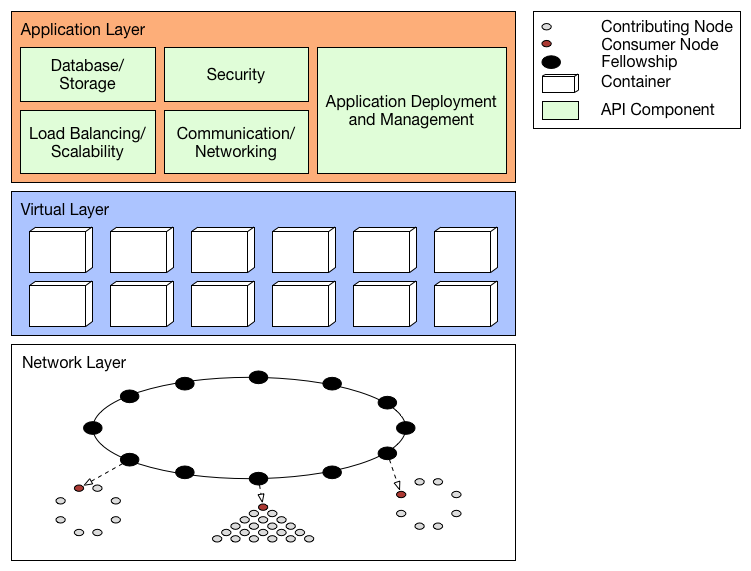
\includegraphics[width=125mm]{images/overview_arch.png}
       \caption{Overview of the Proposed Architecture.}
     \end{figure}
     % End of Figure
     In this architecture we differentiate between 3 types of nodes, namely a \emph{Worker
       node}, a \emph{Data node} and an \emph{Application Deployer node}. A \emph{Worker
       node} consists of a computational resource, executing tasks encompassing \emph{all}
     the functionalities of the applications. Whereas a \emph{Data node} consists of a
     storage resource, performing all the database and storage related tasks. The
     \emph{Application Deployer node}, is the node that contracts contributing nodes to
     host an application in this system.

     Starting at the lowest-level, we have the \textbf{Network Layer}. It is responsible
     for all the network responsibilities including the creation and maintenance of the
     overlays, the communication amongst the participants, and to provide the high-level
     layers with an abstraction of the underlying physical network structure.

     On top of the Network Layer, we built the \textbf{Virtual Layer}. It is
     responsible for abstracting the physical characteristics of each node and providing a
     homogeneous interface to a collection of heterogeneous resources using virtualization
     technologies.

     Finally, the top-most layer is the \textbf{Application Layer}. It exposes an
     \gls{api} to the consuming node used to build applications. This \gls{api} is a
     minimal specification of the services required to transform raw resources into a
     complete computing platform, similar to PaaS computing platforms.

     \section{Network Layer}
     % Topic Sentence:
     In this section we present the \emph{Network Layer} and the rational from which it
     originates, as stated in Section~\ref{arch_over}, it is responsible for providing all
     the networking capabilities for this system. It accomplishes this using two
     abstractions, \emph{the Ring} and \emph{the Fellowship}. We present the two
     abstractions and explain their relevance for this architecture.

     \begin{figure}
       \centering
       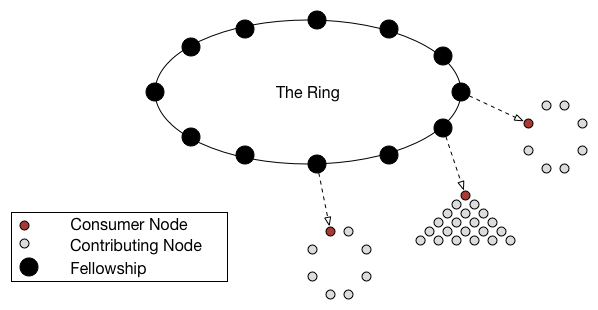
\includegraphics[width=125mm]{images/arch_net_ring_fellow.png}
       \caption{Network Layer Overview}
     \end{figure}

     % Support Sentence: Rationalization of the choice of overlay
     When devising a distributed system, one is confronted with fundamental problems such
     as: \emph{How can we connect a collection of computers, using the Internet, and
       maintain connectivity among them?} From what we have presented in
     Section~\ref{bkg_overlay}, we can address this problem by creating an overlay network
     to connect a collection of computers and maintain connectivity among them. But then
     the question becomes, which topology of overlay network is best suited for our
     requirements, or is it not relevant in this context?

     A case-study presented in \cite{p2p_collab}, outlines the difference between the
     various topologies an overlay network can have in the context of a peer-to-peer
     collaborative system. The authors conclude that \emph{both} topologies of overlay
     networks, structured and unstructured, exhibit different characteristics which can
     be desirable for peer-to-peer collaborative systems, but none of the topologies
     provides a comprehensive solution addressing the requirements identified
     by the authors. Consequently, we know that a single overlay network will not address
     all our requirements of peer-to-peer collaborative systems. Before
     proceeding further lets recall quickly what the two related projects have done to address
     these requirements. If we look at the networking layer for both projects, Cloud@Home
     and \gls{p2pcs} respectively, we notice that the former favors a centralized
     management entity. This entity is used as a central connection end-point, each node
     contacts this entity to be part of the network, and this entity maintains the
     connectivity in the network. The latter focuses primarily on epidemic and
     gossip-based protocols to generate the overlay networks and to maintain
     them. Adopting a slightly different strategy, each application generate and maintain
     their own overlay network (slices) resulting in a federated management structure,
     where each slice is responsible for its nodes.

     In order to respect \textbf{Requirement 3}, as presented in Section~\ref{int_req}, we
     must not opt for a centralized solution, because it introduces a single point of
     failure in the system. We chose a structured overlay network topology for our first
     abstraction, the \emph{Ring}, providing the characteristics and features that are
     desirable for its intended purpose. For our second abstraction, the
     \emph{Fellowships}, we open the possibility to use any overlay network topology.

     In the following subsections we present these abstractions, and we present the
     different design decisions made and the rational behind them.

     \subsection{The Ring}\label{arch_ring}
     % Topic Sentence:
     We have created the \emph{Ring} abstraction to separate the concerns of the publicly
     available portion of the networking infrastructure from the privately available
     portion or the application environment. In this subsection we present the design
     rational, followed by the conceptual manifestation of this abstraction and its
     implications for the architecture.

     \begin{figure}[h]
       \centering
       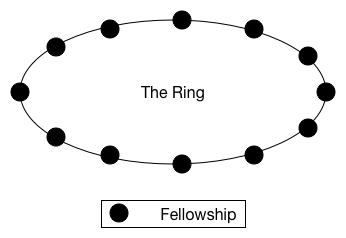
\includegraphics[width=125mm]{images/arch_ring.png}
       \caption{Abstract Representation The Ring.}
     \end{figure}

     % Support Sentence: Why the ring ...
     The necessity of devising an abstraction to encapsulate the \emph{public} environment
     in which our architecture operates, is an attempt to provide a construct that
     exhibits some of the desirable characteristics of a peer-to-peer collaborative
     system. We have identified four distinct features that we deemed desirable for this
     construct:

     \begin{enumerate}
     \item Connecting the participants together in a public environment, such as the
       Internet, resulting in a \emph{public meeting point}.
     \item The management responsibility should not be centralized, as to prevent a global
       system failure occurring as the result of a(ny) subset of participants failing or
       leaving.
     \item Provide querying mechanism to \emph{publicly} locate applications that are
       deployed using this architecture, and ensure its reliability.
     \item Any information that might be required by a(ny) participant to join an application
       should be contained in this construct, and the consistency of the information should be
       ensured to prevent malicious participants from corrupting the information and paralyzing the
       system.
     \end{enumerate}

     In order to provide the first feature, it is clear that an overlay network would
     suffice, independent of its topology. We can use the same rational for the second
     feature, because none of the topologies imposes the centralization of the management
     responsibilities and they can operate in fully decentralized environments. In order
     to provide the third feature, it is necessary to opt for a \emph{structured}
     topology, rather than an unstructured topology. Because, as we have presented in the
     Section~\ref{bkg_overlay}, unstructured overlay networks do not provide a
     deterministic querying mechanism. Furthermore, the last feature entails that this
     construct is fully self-contained and thus, it must possess some storage capabilities
     to store the information.

     Because of its storage capabilities, its deterministic querying mechanism and its
     fully decentralized architecture we opted for a structured overlay network.  As a
     matter of fact, we are using \emph{Kademlia} \gls{dht}, which provides the ability to
     locate any node, deterministically, in a time complexity of $O(log n)$
     \cite{maymounkov2002kademlia}.

     % Support Sentence: restraining writing to appD
     Using this \gls{dht} to store information is intuitive, but using this technology
     into the context of this architecture imposes further constraints. We need to ensure
     that malicious nodes cannot compromise the system by polluting or corrupting the
     information stored in the \gls{dht}. This corresponds to a \emph{storage attack}.
     Essentially, all \gls{dht} are inherently vulnerable to this type of attacks, because
     the design assumes a cooperative environment, where each node is benevolent and most
     implementations do not address this directly, rather they leave it to the application
     developer. For an extensive survey of the security techniques applicable to
     \gls{dht}s, see \cite{urdaneta2011survey}. Thus we require the following changes to
     the \gls{dht}, to ensure consistency and correctness of the information stored in the
     \gls{dht} to an \emph{acceptable} degree. Restraining the writing access of the
     participants, to only those that are \emph{application deployers}\footnote{Further
       information on the types of participants is provided in Section~\ref{arch_over}.},
     reduces the threat model posed by possible storage attacks.

     Then, the problem becomes: how can we ensure the benevolence of the \emph{application
       deployers}? It is not possible to ensure absolute benevolence, but it is possible
     to limit the potential consequences of a storage attack by some malicious writer. We
     limit the application deployers ability to write values, to only two keys. One of
     those keys is named, the \emph{template key}, and it corresponds to a public
     repository containing the attributes a node can use to advertise its resources, be it
     dynamic attributes such as \gls{cpu} usage, or static attributes such as total amount
     of physical memory. Whereas the other key, refers to the application deployed by the
     participant, and can only be written to by this participant, but it can be read by
     all. It contains the list of nodes composing the \emph{Fellowship}, providing the
     ability to a node to reconnect to a previous application following a failure by
     contacting any nodes in the list.

     Ultimately, the implementation of the DHT remains unchanged, and we enforce these
     restrictions in the interface defined for this layer\footnote{More information
       about the interfaces to the different layers in Chapter~\ref{implementation_chap}.}.

     \subsection{The Fellowships}
     % Topic Sentence:
     This abstraction is responsible for the \emph{private} portion of the networking
     infrastructure. We use the word \emph{private} to distinguish between publicly
     available networks, such as the \emph{Ring}, and privately available networks, such
     as the network of contributing nodes for a single application. In this subsection we
     present the design rational for this abstraction and also the conceptual
     manifestation, and its implications for this architecture.

     \begin{figure}
       \centering
       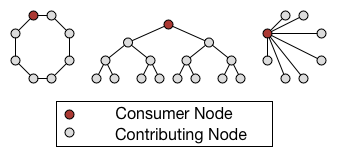
\includegraphics[width=125mm]{images/arch_fellowship.png}
       \caption{Fellowship Abstraction.}
     \end{figure}

     % Support Sentence: design rationale..
     We design this abstraction to have a clear separation between the nodes that
     \emph{are} contributing and the nodes that \emph{wishes} to contribute, by
     segregating them into different networks. This confers the private characteristics to
     this abstraction, and accentuates the modularity of this architecture. Consequently,
     this abstraction needs to account for the following essential features:

     \begin{enumerate}
       \item The ability to discriminate between contracted nodes and malicious nodes
         (pretending to be a contracted contributing node).
       \item Allowing any nodes to join and leave in a graceful fashion, and consequently
         remove any single point of failure.
       \item Providing means for secure communications among the nodes contributing to the
         same application.
     \end{enumerate}

     The \emph{Fellowship} consist of a private collection of nodes interacting together
     exclusively. They are not required to interface with any public environment directly
     as required for the \emph{Ring} when new nodes are arriving.

     Our primary focus, with respect to this abstraction, is the isolation of these
     private application networks, by controlling which participant can join and which
     can't, as expressed in first feature. We can ensure this using a \emph{whitelisting
       mechanism}. The application deployer will create a list, by selecting candidate
     contributors, and will \textbf{only} contract these contributors to host the
     application. This is especially useful in \emph{semi-private} or \emph{semi-trusted}
     environments. A \emph{semi-trusted} environment, is an environment in which the
     different parties (i.e., contributors and consumers) are known to each other
     a-priori, but are connected together through public networks, such as the
     Internet. If it is impossible to establish a semi-trusted environment then other
     means of authentications are required. In a fully untrusted environment, such as the
     open Internet, it is very difficult to ensure the identity of a specific participants
     without any 3rd-party acting as an authority. Although, we could mitigate this by
     implementing a reputation system that would gradually increase the trust component
     for each participants as they contribute \cite{jin2010unstructured}, but we leave it as
     future work.

     For the second feature, we are inclined to implement a similar strategy as
     Peer-to-Peer Cloud System did with the slices. Similarly, we suggest to create one
     overlay network per application, and we do not impose any topology, but rather leave
     it as an application dependent design decision. Since we are not restraining the
     topology of the overlay network, we extend greatly the extensibility and flexibility
     of this architecture, because depending on the application's networking requirements
     a topology might present more advantages over another topology. For example, if your
     application interacts with a plethora of sensing devices distributed geographically,
     an \emph{unstructured overlay network} would provide the ability to aggregate the
     information while flooding or performing random walks through the network, thereby
     providing the ability to perform complex queries. Whereas, a \emph{structured overlay
       network} would require multiple simple queries and post-processing of the results
     in order to aggregate them, achieving the similar results less efficiently.

     The last feature, can be provided by implementing a \gls{pki}, where the application
     deployer is the certificate authority providing public keys to every node, given that
     their identity has been verified by the registration authority, which can (and
     should) also be the application deployer. Then, by using this technology we can
     ensure that the communications are encrypted, certified, and secured.

     Finally, this abstraction provides the ability to control which participant is
     allowed to participate in the collaborative application, but also the ability to
     secure the communication channels using public-key cryptography. Depending on
     the networking requirements of each application, it is possible to tailor the
     \emph{Fellowships} structure to fulfill these requirements.

     \section{Virtual Layer}
     % Topic Sentence:
     In this section we present the \emph{Virtual Layer}, defining its purpose and the
     implications for this architecture. In other words, we present what this layer should
     provide for our architecture and how should it provide it in order to respect and
     fulfill our requirements. We then showcase how our approach differs from the previous
     approaches, used by the two projects evaluated in the Chapter~\ref{rel_work}.

     % What it does...
     There are three essential features that this layer should provide. The first and
     foremost feature this layer should provide, a security mechanism to isolate a
     dedicated execution environment in a contributing host system. It should \emph{sandbox}
     the contributed resources from the contributors operating system, in such a way that
     no matter what gets executed within this \emph{sandbox}, it can never access the
     \gls{os} hosting it or better yet, it cannot know whether it is a virtualized
     resource or a physically dedicated resource.

     Another important feature this layer should provide, is the ability to abstract the
     resources from their underlying physical architectures. Using virtualization, it is
     possible to abstract away the specificities of the underlying physical resource, and
     to present all the resources in an agnostic fashion to possible consumers. In other
     words, it is possible to present two physically different resources, such as a
     computer using a \emph{Intel} \gls{cpu} and a computer using a \emph{AMD} \gls{cpu}
     or even a \emph{ARM} \gls{cpu}, as identical computational resources, distinguishing
     them solely based on their capacities rather then proprietary physical architectures.

     The last feature this layer should provide, is the ability to control and restrict
     the amount of resources contributed to the system. That is, a contributing node
     should be able to restrict its contribution to a desired threshold. Consequently, when
     allowing only a small percentage of the available resources to be contributed, the
     virtualization technology should aim at minimizing its overhead memory footprint as
     to maximize the usage of the contributed resources.

     % What technology present these characteristics?
     Then, the design question becomes, which virtualization technology offers these
     features without compromising our initial research requirements, presented in
     Section~\ref{int_req}. \emph{Light virtualization} technologies, are a potential
     solution to this design question, but let's examine to which extent they are
     different from \emph{full virtualization} technologies.

     As prescribed in the first feature, light virtualization provides the isolation
     required to securely execute applications without interfering or compromising the
     host execution environment. Due to their sandboxing properties, executions done
     inside a container are opaque to the host \gls{os}, as would be the case with full
     virtualization technologies. Thus both technologies, light and full virtualization,
     fulfills this requirement completely. Same goes for the second feature, which is also
     provided by both types of virtualization technologies. Because, both types provides
     homogeneous abstractions for the physically heterogeneous computing resources, and
     both types presents the physical resources in an agnostic way. Still, both
     technologies are equally desirable in the context of the first two features.

     Now we need to look at whether or not it provides the ability to restrict the
     virtualization to a subset of the available computational resources. Docker, one of
     the containerization technology presented in Section~\ref{bkg_docker}, offers this
     functionality using their image system. Using the c-group technology, as presented in
     Section~\ref{bkg_cgroup}, users hosting containers are able to restrict the processes
     spawned within a container to only a specific subset of the available resources. As
     for the full virtualization technologies, it is also possible to restrict the amount
     of resources available to a \gls{vm}, through various configuration parameters. But a
     \emph{difference} ultimately persist between the two types of virtualization
     technologies. By using lightweight virtualization technologies, we can leverage the
     libraries and the kernel of the host \gls{os}, reducing the possible redundancy of
     the libraries and binaries to a minimum, as presented in
     Section~\ref{bkg_virt}. Whereas, using full virtualization technologies, it is likely
     that some of the libraries and binaries are installed twice, once in the \gls{vm}
     itself and another copy could be installed on the host \gls{os}. This outlines the
     major difference between full and light virtualization technologies. Because, by
     design the overhead incurred by full virtualization, with the notion of a hypervisor
     residing on top of the \gls{os} having to translate the requests and commands from
     the \gls{vm}s into intelligible commands for the \gls{os}, is far greater than by
     light virtualization. Because it removes the intermediate hypervisor, and instead
     uses namespace isolation and resource isolation to access the resources directly.

     We conclude that light virtualization technologies are more apt for
     limited-resources, because they provide isolation as well as minimize their memory
     footprints, thereby fulfilling the last requirement.\\

     Using light virtualization technologies is justified due to our specialized
     requirements, and in this interlude we examine how the previous projects (Cloud@Home
     and \gls{p2pcs}) addressed their virtualization requirements.
     % How the other projects approach this...
     If we recall what both projects proposed, we can observe that \textbf{both} advocated
     the use of full virtualization technologies. It provides the desired isolation
     properties, as well as possessing the abstractive capabilities necessary for
     \emph{their} architecture. In the context of \gls{iaas}, it is mandatory to
     resort to \gls{vm}s in order to provide the ability to host an entire
     \gls{os} on the resources, as advertised by this service model.

     We beg to differ with respect to full virtualization as being adequate for
     \emph{every} service model. For a service model akin to \gls{paas}, \gls{vm}s provide
     too much flexibility and extensibility of configuration which complicates the
     application creation and deployment process. It reduces usability by forcing the
     person writing the application to consider details about the configuration of the
     execution environment, across multiple layers rather than only across the application
     and data layers as presented in ~\ref{cloud_sep_of_resp}. Conflating multiple
     concerns ultimately hinders the productivity and the usability of the computing
     platform. We believe that constructing an application using a computing platform,
     such as a \gls{paas}, that this platform is meant to abstract away the
     characteristics of the underlying physical resources, enabling the developer to write
     an application using the interfaces independently of the underlying
     implementations. Whereas full virtualization provides exactly the opposite
     experience, by exposing all the underlying resources, it forces the user to decide
     which implementation to use and how the resources should interact with each other on
     a lower-level.

     Consequently, we choose to use operating system-level virtualization or lightweight
     virtualization, because it satisfies our virtualization requirements, but also vastly
     improves the usability of the system. To the best of our knowledge and in all
     humility we believe to be the first proposing this type of virtualization as a
     integral part of a computing platform.

     \section{Application Layer}
     In this section we present the \emph{Application Layer}, and we present how we came
     about this minimal \gls{api} specification that reflects the essential features of
     distributed computing platforms, such as \gls{paas}.

     Initially we present the reasons for devising this layer, and then proceed to present
     each of the components of composing this \gls{api}: the \emph{Databases and Storages}
     component, the \emph{Communication and Networking} component, the \emph{Load
       Balancing and Scalability} component, the \emph{Security} component and the
     \emph{Application Deployment and Management} component.

     \subsection{Overview}
     The purpose of this layer is to provide to the application developer the necessary
     building blocks to develop a scalable distributed web application. We propose a
     minimal \gls{api} specification that provides these building blocks. It is minimal in
     the sense that it is sufficient to develop most applications, but more features
     can be added to ease the development process of more complex applications.

     By definition \gls{api}s are extensible, since they provide interfaces to the
     functionalities contained, while abstracting away the details of the
     implementations. Using an API to develop applications provides greater modularity
     with respect to the underlying system, because these applications will always be
     compatible with this system even if several update occurs, as long as it respects the
     interface defined initially.

     We have defined the essential components of this \gls{api} by investigating the major
     \gls{csp} that provides a \gls{paas} service model, such as \emph{Google, Amazon, and
       Microsoft}. For more details on the different services offered by the major service
     providers, which served as a basis for this proposed specification, and
     reproducibility's sake please refer to \cite{gae_web} \cite{AWS} \cite{azure}. Then,
     we have identified the overlapping components, and eliminated the \emph{redundant}
     components. Figure~\ref{api_spec_overview} is a pictorial representation of the
     resulting \gls{api} specification.

     \begin{figure}[h]
       \centering
       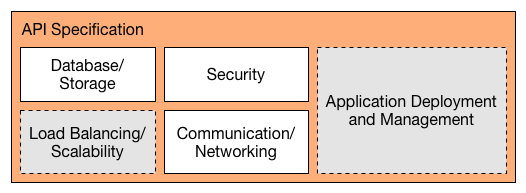
\includegraphics[width=125mm]{images/api_overview.png}
     \caption{API Specification Overview}
     \label{api_spec_overview}
     \end{figure}

     The components identified by a \emph{solid box} are those exposed to the application
     developer, and those identified by a \emph{grayed dashed box} are integral parts of
     the distributed computing platform. The division of concerns is not absolute, and we
     chose to provide access to the components represented by a \emph{grey dashed box} to
     the application developer through configuration parameters rather than building
     blocks.

     In the following subsections we discuss in further details each of the five
     components identified, providing an overview of the functionalities they contribute
     to this architecture and the reason of their inclusion.

     \subsection{Databases and Storages}
     % Topic Sentence:
     The first component of this \gls{api}, is centered around the necessity to
     \emph{persist} data or information in the context of a distributed application. We
     have defined a taxonomy of the primary storage services offered by the major
     \gls{csp}s, and then we discuss the concerns relative to the provision of these
     services and its consequences on this architecture.

     \begin{itemize}
       \item \textbf{Relational Databases:} provides traditional \gls{rdbms}\ facilities.
       \item \textbf{Non-Relational Databases:} commonly referred to as \emph{No-SQL}, this
         type of databases offers schemaless database facilities, such as key-value stores.
       \item \textbf{Storage:} provides all storage needs with larger space requirements
         per entry (up to 1TB) and for heterogeneous objects that usually are represented
         as a binary string (for which the format and content are not relevant and all
         objects are represented as the same type of object). A common way of using such
         storage components is to pair it with a \gls{rdbms}, in which we store the
         meta-data for all the objects stored in the data store. Then this meta-data is
         indexed and associated with a key that represent the location of the actual data
         in the data store.
       \item \textbf{Caching:} provides caching capabilities for fast access to small
         chunks of data, storing them in memory for future access.
     \end{itemize}

     Relational databases, non-relational databases and storage systems in general shares
     similar concerns about \emph{availability}, \emph{reliability}, and
     \emph{consistency} in a distributed environment, and thus we can analyze them in
     parallel.

     In all cases, due to the distributed nature of the underlying compositional
     resources, there is a need to properly \emph{replicate} the persistent data of the
     application, in order to ensure \emph{consistency} and \emph{availability} of the
     data.

     Were we offering a \gls{iaas} computing platform, we would extend concern about the
     distributed nature of the system not only towards databases, but also towards file
     systems, because each component has their own file system. Multiple solutions
     exists, one of which is the distributed file system from Google, the \emph{Google
       File System}\footnote{As a matter of fact, this is exactly what Cloud@Home proposed
       to implement to offer distributed file system capabilities within their
       infrastructure.} \cite{gfs}. But we are focusing on a computing platform that
     shares more in common with \gls{paas} than any other service models, and consequently
     within this context a file system is irrelevant because it is too low-level. Our
     concerns with respect to the distributed nature of the system persists, and
     reliability, availability and consistency must be ensured nonetheless.

     We then resort to \emph{distributed databases}, for which there exists different
     implementations\footnote{We explore these a bit further when discussing the actual
       implementation in Chapter~\ref{implementation_chap}.} that provides a plethora of
     features crossing the boundaries between relational databases,
     non-relational databases and even storage type solutions. Distributed databases
     provide the ability to adjust the availability of the data in response to the
     fluctuations of the number of incoming requests, by adding more instances to the
     database cluster. Distributed databases are devised around two important concepts:
     \emph{replication} and \emph{fragementation}. The former represents the ability to
     replicate the data across several instances, to ensure the availability and the
     consistency of the data. Whereas the latter represents the ability to decompose the
     relations between schema entities into several sub-relations and to distribute them
     across several instances. After which, it is possible to reconstruct the original
     relations using these sub-relations (or fragments), thus balancing the workload
     across the instances. Much more information can be found on distributed databases,
     and to provide an extensive overview of all the characteristics and features of the
     many variations is out of the scope of this thesis, instead refer to
     \cite{linders1976distributed} \cite{draffan1980distributed}
     \cite{ozsu2011principles}.

     Rather than committing this architecture to a single distributed database
     implementation, or even to an implementation for each of these three services
     \emph{(\gls{rdbms}, No-SQL, and storage solutions)}, we opted for an
     extensible design. We provide an universal interface\footnote{We discuss this
       interface in greater details in Chapter~\ref{implementation_chap}.} to these
     database and storage systems, and thus if the solution provided doesn't suit their
     need it is possible to extend the interface to account for other functionalities.

     The last service comprised in this component, is \emph{caching} and it is useful in
     many distributed web applications. Caching consists of a service that enables the
     application developer to store data in a cache for \emph{faster} future access. It is
     primarily used in database-driven web applications, in order to reduce latency by
     caching popular data in-memory, and thus reducing the number calls to external or
     physical data sources. \emph{Memcached} is an example of a distributed caching
     mechanism, allowing to logically combine any unused memory in servers to form a
     bigger unified cache \cite{fitzpatrick2011memcached}. It is open-source, and we can
     provide it as a service without much problems.

     In summary, we provide database and storage capabilities through the implementation of
     an interface, enabling the application developer to quickly integrate any open-source
     and readily available database or storage system implementation. We agree that
     caching is important for data-intensive applications, but we leave the implementation
     of this feature as future work due to the scope of this thesis.

     \subsection{Communication and Networking}\label{arch_comm}
     % Topic Sentence:
     This component is responsible for online accessibility,
     presentation of the information using markup languages, and the communication interface
     between the user and the application.

     But, first, we need to underline that the problem of collaborative web hosting
     remains an open problem in the context of the current Internet's infrastructure. The
     problem revolves around the ability to name the resources in a dynamic distributed
     environment, but also how to provide searching and indexing capabilities in that same
     environment, as well as ensuring content availability.  An extensive reflection
     already exists about this specific problem, and we diligently refer the reader to
     \cite{ahmed2014collaborative} for more information.

     Therefore, we must assume that a domain is already hosted in order to access the
     application using a \gls{url}, or it is accessed using the IP address directly. By
     supporting a web framework, we can provide a service to programmatically present the
     information of the web application.

     We provide a communication interface between the application and the end-user using
     \gls{rest} based \gls{api}s, based on the unanimity amongst the \gls{csp}
     investigated.  \gls{rest}, is a collection of design patterns and guidelines to
     create scalable web services, and it uses HTTP as the underlying communication
     protocol. For a complete account of the guidelines and design patterns present
     in \gls{rest}, see \cite{richardson2008restful}.

     Ultimately, we provide the services for the end-user to communicate with the web
     application using HTTP requests, and provide access to the underlying \gls{rest}ful
     \gls{api}s to the end-user to interact with the web application. A web server
     accessible using the current Internet infrastructure receives these requests,
     providing means to programmatically present the information of the application to the
     user.

     \subsection{Load Balancing and Scalability}
     % Topic Sentence:
     It is common for people to conflate \emph{load balancing} and \emph{scalability},
     because their of semantic similarities relating to their purpose. In other words both
     are concerned with optimizing the performance of the system, but operates at
     different levels. Load balancing consists of distributing the workload as evenly as
     possible across the different resources to optimize the resource consumption. It can
     be achieved by using \emph{task queues} as a service, as shown by the \gls{csp}
     investigated. Whereas scalability differs in how it attempts to optimize the
     performance of the system. Load balancing optimizes the system performance by
     devising the optimal scheduling plan for the current workload. Conversely,
     scalability optimizes the system performance by preempting resources to respond to
     the fluctuations in the workload. The workload could diminish to a point that most of
     the resources are idling, and enforcing scalability would preempt some of
     resources in order to maximize the utilization of the remaining resources, and
     vice-versa.

     In this subsection we present \emph{task queues}\footnote{\emph{caveat lector}: Since
       queues are a fundamental component of this architecture we will only address
       \emph{task queues} as a service or feature to build applications, and then we will
       discuss the details of this architecture in further details in
       Chapter~\ref{implementation_chap}. Because it digresses too much from the service
       offered in the context of the application layer.}, as a service or feature of a
     distributed computing platform. Then we present one, out of many, applicable
     autonomous techniques to achieve scalability in a distributed application.

     \\ Task queues are used to manage the work that happens outside of the normal
     request-response cycle of web applications. Tasks that are queued are handled
     \emph{asynchronously}, in order to prevent interruptions or delays to the
     request-response cycle. Tasks can also originate from other sources, such as
     time-consuming maintenance operations and long-standing background processes A
     workflow commonly used alongside task queues is:
     \begin{enumerate}
     \item Define the maximum request-response interval your application will tolerate.
     \item Evaluate if a job will surpass that interval.
     \item Given that it surpass this interval, schedule a task in the task queue.
     \item Upon completion of the task, store the result in a cache mechanism.
     \item Respond, when possible, by reading the value from the cache.
     \end{enumerate}

     Combining such a workflow with the concept of independent computational entities,
     such as \emph{worker nodes} in a distributed system, monitoring the queues for
     any new tasks to perform, is generally sufficient to distribute the workload across
     the different nodes and to achieve \emph{decent} load balancing.

     These task queues are central to this architecture and this is why we do not provide
     them as a service in the application layer, because it would be redundant. When
     explicitly necessary one could extend this architecture to incorporate any task queue
     implementation of their choice. Although, we acknowledge that we can get into more
     details with respect to load balancing since sophisticated algorithms have been
     proposed to handle different specific cases \cite{antoine2014generic}
     \cite{kansal2012existing}, we deem it to be \emph{application-dependent} and thus not
     as relevant for this minimal specification for an \gls{api}.

     % SCALABILITY

     \\ The other aspect of this component is scalability, we rationalized scalability as
     being the ability to respond to the fluctuations in the workload, either manually or
     autonomously.  The \gls{paas} providers we have investigated, offers the ability to
     the user to specify \emph{static} or \emph{dynamic} policies. These policies usually
     are expressed in terms of \gls{sla}, and ensure that the different \gls{slo} are
     respected by requesting or returning resources accordingly. \gls{sla} are contracts
     that specifies the terms of a service between the consumer and the producer, whereas
     the \gls{slo} are metrics used to measure the service provisioning performance of a
     provider, preventing any misunderstanding between both parties. There are many
     characteristics important when defining \gls{slo}s and forming proper \gls{sla}, we
     focus on a slightly different approach to provide scalability and thus we refer the
     reader to \cite{keller2003wsla} \cite{sturm2000foundations}, for more information on
     service level management.

     We provide scalability by implementing a decentralized autonomic
     controller for each type of node\footnote{see Section~\ref{arch_over}.}, based on
     \cite{gergin2014decentralized}. In order to achieve scalability, the application
     developer will specify it's policies with respect to the utilization of the two types
     of nodes, in the form of a percentage. Using this policy we will attach an autonomic
     controller for each type of node, and it will be used to monitor and make the
     appropriate adjustments in response to the changes in the performance.

     \begin{figure}[h]
       \centering
       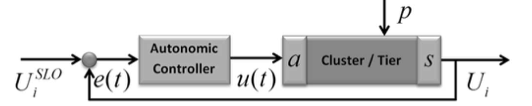
\includegraphics[width=100mm]{./images/self_optimization-PID.png}
       \caption{Proportional-Integral-Derivative (PID) Controller
         \cite{gergin2014decentralized}}
       \label{pid_fig}
     \end{figure}

     The controller used is \gls{pid}, shown in Figure~\ref{pid_fig}, and it operates as
     closed-loop control system. It computes the difference between the desired
     performance $U^{SLO}_i$, described in the \gls{slo} for that type of node, and the
     performance observed $U_i$, which is represented by $e(t)$ in this figure. It will
     interpret the result, $e(t)$, according to this function and return the changes
     required to remain within the $U^{SLO}_i$, denoted by $u(t)$:

     \\ \begin{center}
       $u(t)= K_P e(t) + K_i \int_0^t e(t) dt + K_d \frac{de(t)}{dt}$
       \end{center}\\

     The first component of this controller, is known as the \emph{proportional component}, and
     it adjust the result in \emph{direct proportion} of the delta between the desired
     performance level and the observed performance level.  The second component computes
     the integral of the delta between the desired \gls{slo} performance and the observed
     performance, adjusting the result with respect to the \emph{historical observations}
     relative to the delta. The last component computes the derivative of the delta
     between the desired \gls{slo} performance and the observed performance, attempting to
     \emph{anticipate} the upcoming performance level. Three coefficients are specified to adjust
     the weight of each of those components, and regulate the behavior of the
     controller. It is then possible for the application deployer to only specified the
     desired utilization level for each types of nodes, and this autonomic controller will
     adjust the resources to respond to the fluctuations in the workload autonomously.

     \\ Ultimately, using task queues as an integral part of this architecture and
     leveraging decentralized autonomic controllers, we are able to provide autonomic
     scalability and efficient load balancing. The load-balancing component is considered
     to be \emph{application-dependent}, because there are multiple factors to take into
     account and it poses a multi-dimensional optimization problem which is not trivially
     solved. This optimization problem yields different solutions in different contexts,
     and different applications requires different solutions. Thus, we provide some
     functionalities as intrinsic features of our architecture, but we leave the more
     sophisticated functionalities to be provided by the application developer.

     \subsection{Security}
     The Security component is concerned with providing means to establish/entertain
     \emph{secure communication channels} between the different nodes, but also between
     the end-user of the application and the node responsible of handling the
     requests. Another major concern is access control, including \emph{authentication} of
     the end-user and providing \emph{multi-tenancy}. We present each of these concerns,
     and explain how they are accounted for in this \gls{api}.

     \\ The first concern is to provide means for secure communication between the
     nodes. It can be ensured using standardized technologies such as communicating over
     TCP/IP using \gls{ssl}. \gls{ssl} certificates are usually negotiated between a web
     server and a client. In the context of this architecture the web server is
     (\emph{usually}) hosted on the application deployer node and the client is a
     candidate node. Consequently, a candidate node would negotiate its certificate with
     the application deployer to establish a secure communication channel between
     them. Upon successful negotiations the node and the application deployer are able
     to communicate securely using the \gls{ssl} protocol.

     The communications between the end-user and the web server can also be secured using
     standardized protocols, by communicating using \gls{https}, which consists of using
     \gls{ssl} on top of HTTP. The negotiation for \gls{ssl} certificates would be done
     between the web server and the end-user. We use well established standard
     technologies (SSL, HTTPS, etc.), as would any other web application when
     required to communicate over unsecured networks, such as the Internet.

     \\ Access control is another important security concern, controlling access to
     resources based on various schemes, using \emph{authorization} mechanisms and
     \emph{authentication} mechanisms. We can identify two basic types of accesses in our
     architecture: \emph{access from node to node} and \emph{access from end-user to the
       web application}.

     The first type of access is illustrated using this example. If we introduce a
     \emph{Byzantine} node, that is a node for which the requests or responses are
     incorrect, either because of an error in the computations or by malicious intent, and
     it requests to drop all the tables in the database. How do we differentiate between
     this request being erroneous or malicious in intent, and a legitimate request to drop
     all the tables? There exists multiple schemes and strategies to enforce various level
     of access control \cite{dara2014multi} \cite{gollman2010computer}, and depending on
     the context in which the application is deployed it can vary substantially. Thus, we
     implement a pragmatic strategy for access control, where only the application
     deployer is allowed to perform administrative tasks. This is known as \gls{mac}
     \cite{nyanchama1995modeling}. The identity verification is done using a simple
     challenge-response between the nodes to assess the identity.

     The second access type, refers to the authentication of the end-users interfacing
     with the application deployed. Authentication, as a service for applications,
     \emph{can} be provided using \gls{sso} technologies. For example, incorporating hooks
     to the Google \gls{sso} \gls{api} provides the ability to the application deployer
     offload the authentication responsibilities, using a \emph{delegation protocol} such
     as OAuth 2.0 \cite{jones2012oauth}, to a trusted third-party. Upon authentication,
     the user will receive a \emph{OAuth} token, also known as a \emph{bearer token}. When
     interacting with the application, the user presents this token to demonstrate its
     identity as certified by the trusted third-party. These tokens have are valid for a
     certain period of time, after which the user is required the obtain a new token. The
     user will also be able to maintain a session using this token. For more information
     on Google's \gls{sso} \gls{api}, see \cite{google_sso}.

     Authentication can be application dependent. Some prefer resorting to a 3rd-party to
     provide authentication, whereas others may prefer holding the credential in a
     database and enforcing authentication themselves. It really depends on the security
     requirements of the application, and thus we leave the responsibility to the
     application developer to provide control over this type of access.

     \\ This leads to the final portion of the security component, \emph{multi-tenancy},
     consisting of the ability to provide parallel multi-user support for an application
     without providing each user with a dedicated instance of the application.
     Consequently, seasoned web developers will find using this architecture very
     intuitive, because instead of forcing sophisticated design patterns, resulting in a
     steeper learning curve, we favor the use of \emph{sessions} to achieve
     multi-tenancy. By using one session per user, it is possible to encompass all the
     information specific to this user in a self-contained web primitive.

     \\
     Finally, we provide secure inter-node communication via SSL, whereas secure
     communication between the end-user and the web application via HTTPS. The access
     control scheme provided is minimal and only the application deploying node has the
     ability to perform administrative tasks. We provide multi-tenancy by maintaining
     parallel user-sessions, which are provided using a \gls{sso} service from a trusted
     third-party or maintained by the web server.

     \subsection{Application Deployment and Management}
     This component encompasses all that pertains to the administrative tools to manage an
     application. Due to the distributed nature of our architecture, we are faced with a
     challenge foreign to current \gls{paas} providers and it is related to
     \emph{source-code distribution}. Every other service in this component, can be
     commonly found in most of the \gls{paas} providers, notably \emph{application
       configuration} and \emph{various monitoring capabilities}.

     \\ The distribution of the source-code of the application is a security concern.
     Because of the distributed nature of the infrastructure it entails that a
     contributing node trusts the application deploying node and the source-code
     distributed. Multiple sophisticated scheme exists to \emph{reduce} the trust-level
     assumed between parties, with regard to source-code distribution, in a distributed
     context.

     One example consists of creating \emph{bundles}, or atomic units, of code and data,
     which can then be distributed and executed \cite{dearle2004flexible}. This deployment
     framework provides authentication and authorization mechanisms, and certifying
     capabilities, creating a trust environment where source code can be distributed and
     executed securely. An undesirable consequence, is that it forces a complete
     deployment infrastructure into the architecture. Applications are required to be
     designed respecting a set of guidelines, leaking into the development process and
     impeding the flexibility of the architecture.

     Instead, we propose a way of providing similar guarantees, that ultimately relies on
     the users judgment and effectively removes any trust factor. Because we provide an
     open-platform, we apply the same open-source principles\footnote{Adopting a similar
       perspective to the Free Software Foundation, who promotes free software and open
       source development, ensuring maximal transparency \cite{fsf}.} to the application it
     hosts by adopting a \emph{white-box} approach. The workflow of distributing code can
     be summarized as follows:
     \begin{itemize}
       \item Application deployer stores the source-code into a public or private
         repository supporting any version control (git, mercurial, svn).
       \item Upon contracting a node for contribution, the application deployer provides
         the location of the application repository to this node, and any credentials if necessary.
       \item The contributing node will then be notified of its content, by presenting the
         source-code in a text editor or browser.
       \item The contributing node is then asked whether or not it accepts to execute this
         piece of code (in a container).
       \item Finally, depending on the response, the code will or will not be downloaded
         into the container (and all of its dependencies).
     \end{itemize}
     This workflow is designed to work in a fully untrusted environment. In a trusted or
     semi-trusted environment (cluster or private network), we can simply turn this option
     off and upon contracting a node for contribution the source-code is directly
     downloaded into the container, implicitly assuming that the user accepts to execute
     its content.

     \\ The \gls{csp} investigated offers application configuration services using a web
     portal that lets the user adjust the different configurable parameters of their
     application. The configurable parameters varies depending on the \gls{csp} and are
     largely dependent on the underlying proprietary technologies used. We offer
     \emph{application configuration} using configuration files. The configurable
     parameters includes: minimum number of nodes, performance policies, type of
     environment deployed, any communication primitives and any security
     primitives. Before the creation of a node instance, its configuration file is read
     and interpreted. This configuration mechanism is easily extensible and could
     compensate for any other requirements.

     \\ \emph{Monitoring} is an important feedback mechanism for the application deployer,
     it is primarily used to anticipate possible bottlenecks or the track the resource
     consumption of the application. We provide monitoring capabilities by implementing a
     heartbeat mechanism, in which every nodes periodically sends information for a
     collection of (user-defined) dynamic attributes. Then the information is collected
     and aggregated, presenting the result as system-wide monitoring information to the
     application deployer. This mechanism provides a sufficient perspective of the
     application state, with respect to the load-balancing and scalability mechanism
     presented earlier.

     \\ In summary, we provide a flexible workflow for code distribution adopting a
     \emph{white-box} approach. We provide the ability to statically configure an
     application through various parameters. We provide monitoring capabilities using a
     heartbeat mechanism that generates system-wide information, using locally available
     information from the participants.

     As future work, we intend to provide dynamic configuration capabilities, in which the
     nodes will be able to modify the configuration parameters dynamically, when
     applicable. Providing a visual representation of the data monitored, using graphs to
     represent the topology and various metrics, would also be desirable from a user
     experience point of view.

     \section{Component Interaction}
     % Topic Sentence:
     In this section we present a way to reason about developing applications that is
     central to this architecture, representing the main interactions between the different
     components of a distributed application.

     % Support Sentence: Logical rationalization of the workflow
     When creating an application using this architecture, it is fundamental to reason
     about the problem at hand in terms of the request-response cycle, that is inherent to
     web applications. This enables the developer to understand how to formulate a
     problem into a compatible solution, using the different constructs available with
     this architecture. We can reason about a distributed application as
     follows:
     \begin{enumerate}
       \item \textbf{(Incoming Web Request)} A user send a request to the web server. 
       \item \textbf{(Generate HTTP Request for App.)} Web server receives the incoming
         request, then formulates a HTTP POST request using the content of the original request,
         and sends it.
       \item \textbf{(Incoming RESTful API Request)} A node receives a request from the
         web server, using a web protocol.
       \item \textbf{(Create Task)} It extracts the information from the request, creates
         a task and queue it up.
       \item \textbf{(Task Available)} Upon queuing the task, it becomes available for
         offloading. It is then dispatched to any available nodes.
       \item \textbf{(Task Completion)} Upon completing the task, the node sends the
         result to the dispatcher of the task.
       \item \textbf{(Task Returns)} Upon receiving the results, the original dispatcher
         of the task uses a web protocol to formulate a HTTP POST request containing the
         results, and sends it back to the web server.
       \item \textbf{(Result Returns)} Finally, the web server receives the result and
         formulates the appropriate response to present the information back to the user.
     \end{enumerate}

     % Support Sentence: Event-Driven Architecture
     Writing applications for this architecture forces an event-driven programming model,
     resulting in applications designed using the \gls{eda} approach. For a distributed
     application, we can identify four logical event flow layers of any \gls{eda}, as
     presented in \cite{michelson2006event}:
     \begin{itemize}
     \item \textbf{Event Generator} is the source of (all) the events, it is the web server
       in the case of web applications.
     \item \textbf{Event Channel} is the medium used to transport events from generator(s)
       to event processing engine(s). In our architecture the event channel corresponds to a
       web protocol, where the incoming events from the generator are used to derive the
       task(s) to be sent to the event processing engine(s). At a higher-level, we say that
       the application deployer itself is the event channel, but more precisely the web
       protocol does the translation from raw events into events that can be processed
       using this architecture.
     \item \textbf{Event Processing} is done by the \emph{event processing engines},
       taking the appropriate actions in response to the events. In our architecture, the
       contributing nodes are the \emph{engines} and they process task(s), which are a
       derived form of events.
     \item \textbf{Downstream Event-Driven Activity} is the downstream activity initiated
       by an event, and it occurs upon processing the event. In our architecture, it
       consists of returning the result of the completed task to the node that dispatched
       it, and can trigger a series of collateral events.
     \end{itemize}

     It is possible to distinguish between different types of event flow processing,
     either \textbf{simple}, \textbf{stream} or \textbf{complex}. Some simpler problems
     impose only \emph{one} event generator, corresponding to \emph{simple event flow
       processing}. Whereas, more complex problems incur \emph{multiple} event generators
     or introduce \emph{continuous streams} of events, corresponding to \emph{complex
       event flow processing} and \emph{stream event flow processing} respectively
     \cite{michelson2006event}.

     % Concluding Sentence:
     Using this kind of reasoning, it is possible to effectively separate the 
     presentation logic from the business logic. We now have a clear understanding of the
     role of both types of nodes: the application deployer will contain the \emph{event
       generator} and will be responsible to dispatch the events using the \emph{event
       channel}. It will also use the event channel to handle any \emph{downstream
       event-driven activities}. Whereas the contributing nodes will only serve as
     \emph{event processing engines}. This rationalization of our architecture is
     crucial to ensure: proper understanding of the problem domain, how to appropriately
     separate the presentation logic from the application logic, and to avoid possible
     design mistakes that could impede scalability.

     % MAY NEED TO PUSH IT ELSEWHERE!
     \section{Discussion}
     In this section we present a discussion of all the layers, and how they contribute in
     fulfilling the requirements of both the evaluation framework, as presented in
     Section~\ref{rel_EvalFramework} and the requirements of this thesis, as
     presented in Section~\ref{int_req}.

     \subsection{Collaborative Peer-to-Peer System Framework Implementation}
     Section~\ref{rel_EvalFramework}, presents a framework that illustrates the essential
     functionalities required for a peer-to-peer collaborative system to scale, by
     mitigating the complexities inherent to these type of systems. This subsection aims
     at presenting the different mechanisms implemented in our architecture to provide
     such functionalities.

     If we recall, the framework was composed of 7 key phases relating to the life-cycle
     of a participant in a peer-to-peer collaborative systems, which were:
     \emph{Advertise}, \emph{Discover}, \emph{Select}, \emph{Match}, \emph{Bind},
     \emph{Use}, and \emph{Release}.

     \\ The first two phases, \textbf{Advertise} and \textbf{Discover}, which relates to
     the advertisement and discovery of resources via formal specification, are
     implemented as a best-effort mechanism. By this we mean that the newly arrived nodes
     create a \emph{Resource Specification (RS)} using a common template, and it can be
     represented as follows:

     %%%%%%%%%%%%%%%%%%%%%%%%%%%%%%%%%%%%%%%%%%%%%%%%%%
     %     %      %     %     %     %     %     %     %
     % IP  % Port % SA1 % ... % SAn % DA1 % ... % DAn %
     %     %      %     %     %     %     %     %     %
     %%%%%%%%%%%%%%%%%%%%%%%%%%%%%%%%%%%%%%%%%%%%%%%%%%

     \begin{center}
     $RS(node_i) = [IPaddress, Port, SA, DA]$ where \\
     $SA = \left\{{StaticAttribute_1, ..., StaticAttribute_n}\right\}$ and \\
     $DA = \left\{{DynamicAttribute_1, ..., DynamicAttribute_n}\right\}$
     \end{center}

     Note that the set of \emph{Static Attributes} and \emph{Dynamic Attributes} are
     extensible to accommodate any desirable attributes, and are initially empty. Each
     application deployer publish any desired attributes to a common repository (or
     in the context of a DHT, append the values to a specific key used by all nodes to
     construct their resource specification simply known as the \emph{template}).

     Upon creating their resource specification, the nodes gather the list of application
     deployers using the \emph{Ring}, and periodically send candidacy messages, containing
     their resource specification. We say best-effort, because the nodes send repeatedly
     their candidacy messages, until an application deployer contracts them for contribution.

     Other solutions proposes to publish resource specifications to a repository where it
     is possible for the consumer to query the repository for the most relevant resources
     \cite{p2p_collab}. These solutions are adequate if the repository is protected
     against possible storage attacks, this is not the case for \gls{dht}s
     \cite{urdaneta2011survey}. Our mechanism enables us to mitigate the possible storage
     attacks, without having to resort to centralized management of the repository,
     because we do not persist the information.

     \begin{figure}[h!]  
     \begin{sequencediagram}
       \small
       \newinst[2]{node}{:Node}
       \newinst[2]{ring}{:Ring}
       \newinst[2]{appd1}{:AppD1}
       \newinst[2]{appd2}{:AppD2}

       \begin{messcall}
         {appd1}{publish(template)}{ring}
       \end{messcall}
       \begin{messcall}
         {appd2}{publish(template)}{ring}
       \end{messcall}
         
       \begin{call}
         {node}{get(template)}{ring}{(template, value)}
       \end{call}
       \begin{call}
         {node}{getAppDList()}{ring}{appDList}
       \end{call}

       \begin{sdblock}{Loop}{pub-sub}
         \begin{messcall}
           {node}{publish(RS)}{appd1}
         \end{messcall}
         \begin{messcall}
           {node}{publish(RS)}{appd2}
         \end{messcall}
       \end{sdblock}
     \end{sequencediagram}
     \caption{Advertise and Discover Phases Sequence Diagram.}
     \end{figure}



     \\ The \textbf{Select} phase relates to the selection mechanism offered to possible
     consumers to query the resource specifications. In this architecture, in order to
     select a node, an application deployers must open a TCP/IP server connection on a
     specific port, and evaluate the upcoming candidacy messages individually by examining
     its content. As a matter of fact, this selection mechanism resort to a
     \emph{publish-subscribe} messaging pattern, where the nodes are the publishers and
     the application deployers are the subscribers. The application deployers are then
     allowed to subscribe only to a \emph{meaningful} subset of the attributes published
     as part of a resource specification, representing a \emph{topic}. The nodes uses the
     concept of topics to publish the various attributes that compose the resource
     specification. Then, application deployers will do a tentative selection, notifying
     the resources that it considers them as candidate resources. The selection is
     completed only after all the required resources, to host the application, are
     \emph{tentatively selected}. This is a blocking operation and can be deferred to a
     background thread, and automated by defining a selection policy. This policy contains
     the desired values for the static attributes, and the intervals of desired values for
     the dynamic attributes.

     \begin{figure}[h!]  
     \begin{sequencediagram}
       \small
       \newinst[3]{node}{:Node}
       \newinst[3]{appd}{:AppD}

       \begin{messcall}
         {appd}{tentativelySeclect()}{node}
       \end{messcall}

       \begin{call}
         {appd}{evaluateSelection()}{appd}{result}
       \end{call}

       \begin{sdblock}{alt}{result != ok}
         \begin{messcall}
           {appd}{not selected!}{node}
         \end{messcall}
       \end{sdblock}
       \begin{sdblock}{alt}{result == ok}
         \begin{messcall}
           {appd}{selected!}{node}
         \end{messcall}
       \end{sdblock}
     \end{sequencediagram}
     \caption{Selection and Match Phases Sequence Diagram.}
     \end{figure}

     \\ The next phase is \textbf{Match}, it encompasses the ability to formally
     specify the inter-resource relationship requirements and to enforce them on the
     selection of resources. As a consequence of using a best-effort mechanism, it is
     possible to define these relationships as an integral part of the selection
     policy. For example, once a group of resources is \emph{tentitavely selected}, it
     is \emph{then} possible to enforce these inter-resource relationship requirements,
     and repeat the process until the \emph{tentative selection} fulfills all the
     requirements in the selection policy.

     \\ The \textbf{Bind} phase, is also best-effort, because of the mechanism in the
     \emph{Select} phase. The priority for an application to contract a specific node is
     determined with respect to the time of the response to a candidacy message. In other
     words applications which responses were received first are given priority, by the
     contributing node, over applications which responses were received later.

     \\ The \textbf{Use} phase states that it should be possible to use the resources
     contracted in the previous phase to execute the tasks pertaining to the
     application. It is accomplished by sending tasks to be executer after that the
     enrollment process (selection, binding, handshaking, initialization of the node) has
     completed.

     \\ The \textbf{Release} phase is concerned with providing the capability to release a
     resource after contributing, either because its \gls{sla} prescribes it or because
     the workload has diminished to the point that this resource is no longer
     needed. Depending on the \gls{sla} between the application deployer and the
     contributing node (encompassed in a policy), release will happen if
     possible. Releasing a contributing node consists of a node leaving its current
     fellowship and returning to the ring, to advertise its resources again.

     \\ Future work includes providing more extensive functionalities for each of the
     phases. We do not include extend these functionalities, because the mechanisms described
     above are sufficient to operate the system efficiently.

     \subsection{Research Requirements}
     We now present how the research requirements were fulfilled in our architecture, and
     present a very high-level recapitulation of the various layers. \\
     
     \textbf{Requirement 1} states that a collection of heterogeneous devices can use this
     architecture to deploy multiple applications simultaneously. It is satisfied by the
     design of the Network layer, because we provide multi-application support using the
     \emph{Ring} and we do not impose any restrictions on possible contributors, as long
     as they meet the light virtualization requirement of being able to host a container,
     which inherently all Linux \gls{os} are capable of.
     
     \textbf{Requirement 2} states that this architecture should not impose third-parties
     to provide any of its services, and this architecture should be self-contained. It is
     partially satisfied by the Application layer, because it does not introduce any
     third-parties\footnote{We do admit that web hosting has to be outsourced, but as we
       stated earlier in Section~\ref{arch_comm}, it remains an open-problem because of
       the underlying infrastructure of the Internet. For a more complete presentation of
       the problem see Section~\ref{probs}.} to provide any of the services
     described in the \gls{api}. Then, we satisfy the remaining portion of this
     requirement, providing the desired self-containment properties using light
     virtualization.
    
     \textbf{Requirement 3} states that this architecture should not introduce any single
     point of failure and should be fault-tolerant to ubiquitous failures of different
     participants. The \emph{security} component\footnote{In no way is this component
       providing \emph{absolute} security to this architecture, and more attack vectors
       need to be analyzed to account for a realistic threat model.} of the \gls{api}
     specification satisfies a portion of this requirement, by providing secure
     communication channels and enforcing \gls{mac} to regulate and control the
     administrative tasks. The \emph{Ring} satisfies the remaining portion of this
     requirement, because it provides the ability to create and maintain a decentralized
     structured overlay network to connect the nodes.

     \textbf{Requirement 4} states that no special or dedicated equipment should be
     necessary to participate in this system. It is satisfied because there are no
     explicit or implicit restrictions on the intended hardware to be used with this
     architecture. Consequently, recycling the currently available hardware is the most
     cost-efficient and eco-efficient, \emph{ceteris paribus}, alternative to participate
     in this system.
     
     \textbf{Sub-Requirement 4.1} states that the memory footprint should be sufficiently
     small to allow lower-end devices to be an integral part of this architecture. It is
     satisfied to the extent that it reduces the overhead induced by the virtualization
     technology to a \emph{smaller} footprint.
     
     \textbf{Requirement 5} states that this system should provide \emph{dynamic
       membership} capabilities as well as scalability to the applications that are
     deployed. This requirement is satisfied using task queues as a foundational construct
     of this system, but also by providing dynamic membership capabilities through the use
     of autonomic controllers to regulate the load on the resources.

     % \subsection{Network}
     \\ We can make the following observations concerning the \emph{Network layer}. Using
     the \emph{Ring} and the \emph{Fellowship} abstractions, we are able to separate the
     concerns of public-resource pooling and resource provisioning. Furthermore, we are
     able to provide fully isolated multi-application support using the
     \emph{Fellowships}. Subsequently, the \emph{Network layer} can be easily adapted to
     different environments (cluster, grid, or open Internet) without incurring any major
     changes, but by simply selecting which underlying networking primitive is a better
     fit. As an example, when operating in a highly dynamic environment (Internet), using
     a unstructured overlay network might be better to cope with the higher churn rate,
     but when operating in a moderately dynamic environment (shared-cluster) using the
     current DHT implementation would be more than sufficient to cope with the moderate
     churn rate.

     %\subsection{Virtualization}
     \\ The \emph{Virtualization layer} uses lightweight virtualization technologies to
     abstract the resources from their underlying physical specificities, providing
     isolation guarantees similar to full virtualization technology. We can define the
     environment of an application and all its dependencies using a single configuration
     file, easing the portability, and creating a fully self-contained deployable
     construct. We are aware of the security concerns related to lightweight
     virtualization technologies, especially because it has direct access to the Linux
     Kernel's system call interfaces. This means that if a vulnerability exists in one of
     the system call interface, then it is possible to exploit it from within a
     container. This can be addressed by applying security profiles, such as Linux's
     \emph{seccomp}, to restrict the breadth of accessible interfaces to a selection of
     safe and tested system calls. Docker applies this approach to augment the security of
     its containers and encourage the developer to be aware of these possible exploits
     \cite{docker_security}.
     
     %\subsection{Application Layer}
     \\ The \emph{Application layer} provides a minimal \gls{api} specification for
     distributed computing platforms, including \gls{paas} platforms, by providing the
     essential components required to develop distributed applications and an
     extensible \gls{api} for all the other non-essential components.
     % END--------------------------

     \chapter{Implementation}\label{implementation_chap}
     In this chapter we present an implementation of the architecture proposed in the
     previous chapter. In order to provide context, we present the technologies used to
     implement the architecture and how they influenced the design, when applicable. We
     then present the central constructs of this architecture, followed by the algorithms
     and workflows used to provide the underlying logic composing this
     architecture. Finally, we present a very simple proof of concept that illustrates the
     orchestration of these constructs and algorithms.

     %\emph{Caveat-lector}: this
     %architecture is designed as a platform for web application (involving a
     %request-response cycle), but is not limited to, for the purpose of this thesis we
     %will only consider this type of application.

     \section{Technology Used}
     % Topic Sentence %
     We have used different technologies in concert to provide the ability to develop
     applications that can be deployed using this architecture.\\
     % Support Sentence: Twisted + Event-Driven Programming Model %

     The code was written using Python and the Twisted Event-Driven Networking Framework
     \cite{twisted}. We adopted an \emph{event-driven programming model}, because it
     provides the ability to reason about problems from a non-sequential perspective,
     which is useful when implementing distributed applications due to their
     complexity. Event-driven programming is conceptually single-threaded, although
     multi-threading is supported by Twisted it is not mandatory, and it is offered as an
     extra feature.

     The primary advantage of using the event-driven programming model lies in its use of
     a single control thread to interleave multiple tasks, resulting in an opportunistic
     event-driven execution scheme. Whereas, a single-threaded program executes tasks
     sequentially, forcing the program to pause its execution at every blocking operation,
     until their completion. This sequential programming model effectively augments the
     total execution time, by introducing gaps in the timeline spent waiting (idling) for
     a blocking operation to return.

     % Support Sentence: Event-Driven vs. Multi-Threaded
     Thus, the event-driven programming model reduces the complexity inherent to the
     development of distributed applications, focusing on the possible events and their
     appropriate responses. Whereas the multi-threaded programming model, consists of
     using a collection of threads to accomplish different tasks, in parallel, and
     requires complex concurrency and synchronization mechanisms. 

     Ultimately, the event-driven programming model benefits from parallel execution of
     tasks, similarly to the multi-threaded programming model, and it combines the
     simplicity of the single-threaded programming model by resorting to a single control
     thread. Figure~\ref{multi} illustrates the distinction between these three programming
     models.

     \begin{figure}[h]
       \centering
       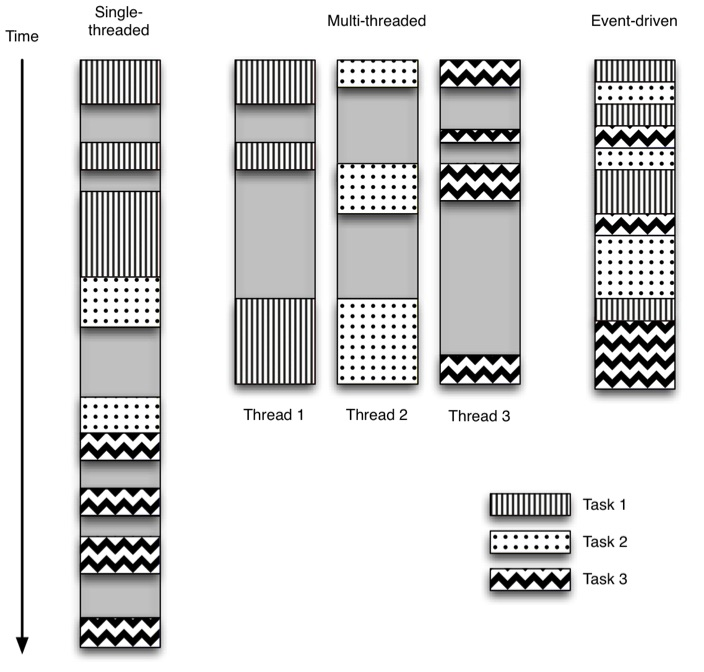
\includegraphics[width=100mm]{images/twisted_multi.jpg}
       \caption{Comparison between Programming Models. \cite{mckellar2013twisted}}\label{multi}
     \end{figure}

     Twisted leverages the event-driven programming model by inter-leaving multiple
     blocking operations and responding to consequential events, such as completion or
     failure, using callbacks. A \emph{callback} is a function to call upon the occurrence
     of an event to handle the results. Twisted allows the developer to specify a callback
     to handle the successful completion of an event, and a callback to handle the failure
     of an event; both are encompassed into the \emph{Deferred} abstraction. Twisted
     orchestrates the callbacks, contained in different deferreds, by registering them
     with an event-loop, called the \emph{Reactor}. This event-loop controls the thread of
     execution, enabling operations to block, and keeping track of which callback is
     associated with which operation. Upon completion (or unblocking) of an operation the
     event-loop is notified and it passes the result to the corresponding callback, to
     be processed. By chaining callbacks, it is possible to achieve very complex asynchronous
     behavior in a cooperative fashion which is at the heart of the philosophy of the
     Twisted framework.
     % Support Sentence: Task --> Deferreds
     The concept of deferreds influenced the design of the constructs composing this
     system and their interactions among each other.\\

     % Support Sentence: Overlay Network --> Kademlia
     The overlay-network used for to \emph{The Ring}, is a Python implementation of the
     Kademlia DHT using \emph{Twisted} \cite{kademlia_python}. Our decision was based on
     the fact that it was implemented using \emph{Twisted}, and it could be easily
     integrated to our architecture incurring minimal disruptions. Another benefit, is to
     have uniformity in the programming-model used throughout the architecture, by
     focusing on the event-driven programming model.

     % Support Sentence: WebServer --> CherryPy
     For the web server, we used CherryPy, a minimal Python Object-Oriented Web Framework
     \cite{cherrypy}, because of its simplicity and illustrative capabilities. It enables
     us to use a web server, without any bloating features and focuses strictly on what is
     necessary, easing the development of prototypes and proof of concepts. We can
     substitute this web framework with a more complete web framework, incurring only
     minimal changes by using our clearly defined interfaces.

     % Support Sentence: Virtualization --> Docker
     To provide virtualization capabilities to the nodes we used Docker Containers
     \cite{docker}. Docker provides self-containing capabilities to each node, by
     specifying the dependencies inherent to this architecture and the dependencies of the
     applications developed, using \emph{DockerFiles}. They act as configuration files,
     prescribing the requirements of the environment, all the dependencies, and the
     quantification of the resources available to execute the containers.

     % Concluding Sentence:
     Using these technologies we were able to quickly and efficiently create
     prototypes, while constructing a solid foundation for this architecture. This
     foundation is the result of creating well-defined interfaces between the various
     components, accentuating the modularity and maximizing the extensibility of this
     architecture.

     \section{Constructs}
     In this section we present the fundamental elements of this architecture, namely
     the \textbf{Task}, the \textbf{ApplicationNode}, the \textbf{Ring} and the
     \textbf{Fellowships}.  We present each of the elements and discuss their
     practical implementations.

     \subsection{Task}\label{impl_constructs_task}
     % Topic Sentence:
     There is a need to represent a series of consequential actions resulting from an
     incoming request, into an easily distributable and self-contained entity. This entity
     \emph{must} provide the ability to return a response to a requester, without any
     ambiguity regarding the originator of the request in the presence of large amount of
     requests.

     % Support Sentence: Task and Deferreds
     Tasks are heavily inspired by Twisted's concept of \emph{Deferreds}, because they
     make similar promises. As we have shown earlier, a \emph{Deferred} promises to
     eventually return from a blocking operation with a result, and to apply the
     processing logic, in the form of callbacks, to this result. Similarly, a task
     embodies this promise of eventual completion and provides the ability to specify the
     result processing logic. As a matter of fact, \emph{Deferreds} are used to chain the
     various processing steps for any given task. Upon the creation of a task, a
     \emph{Deferred} is attached to it, consisting of the processing logic that must be
     applied when this task is dispatched to a node. The principal function required to
     process this unit of work, is the first callback to be chained in the callback chain
     of the \emph{Deferred}. Then, any subsequent post-processing function will be chained
     to that same callback chain, representing the complete sequence of operations.
     % Support Sentence: Task atomicity and taxonomy
     A task corresponds to an atomic unit of work in this system. Analogous to the
     database atomic transaction property, a task can be in one of two states, completed
     or not processed at all. Task(s) are fully self-contained and stateless in the sense
     that any task can be dispatched to any node, without having to synchronize the
     states of the nodes, receiving the task is sufficient to execute it, and carry out
     the corresponding sequence of operations. We distinguish between two types of tasks, a
     \emph{Worker Task} and a \emph{Data Task}. The former consists of \textbf{ANY} type
     of computational task, whereas the latter consists of task that pertains to
     persistent data (either storing or retrieving data).
     % Support Sentence: Task dynamic linkage
     Task objects are simple constructs containing the parameters, the module and the
     function names related to a unit of work. Once created they are dynamically linked to
     the module provided and the corresponding function.

     % Support Sentence: Task Functions
     A \textbf{task function} takes 2 parameters: a \emph{task object} and a
     \emph{list of arguments}. Where the former is the instance of the task itself, and
     the latter is any parameters that are necessary to execute this function. Thus, a
     normal function can be refactored into a task function simply by modifying the
     signature of the function to take only the \emph{task object} and a list
     representation of all the (current) parameters; and include logic to extract the
     parameters from the list. \clearpage
     Here is an example of a simple arbitrary function:
     \begin{python}
       def arbitraryFunc(op1, op2):
         return op1 + op2
     \end{python}
     And here is this function re-factored to be a task function:
     \begin{python}
       def arbitraryFuncTask(taskObject, params):
         op1 = params[0]
         op2 = params[1]
         
         taskObject.results = op1 + op2
         taskObject.completed = True

         return taskObject.completed
     \end{python}

     % Concluding Sentence:
     Developing applications by defining the business logic into self-contained units of
     work, helps mitigate a large portion of the complexity inherent to distributed
     systems, but imposes a fairly strict programming model on the developer. Such a
     programming model may be difficult to abide to in some cases, notably where the
     services provided by an application cannot be easily parallelized or exhibit inherent
     serial properties.

     \subsection{ApplicationNode}
     % Topic Sentence:
     This construct represents any participating node in the network,
     and distinguishes between application deployers, and contributing nodes.

     % Support Sentence: Application Deployer
     \textbf{Application Deploying Nodes} are the nodes contracting the contributing nodes
     in order to host an application using this system. Hosting, in this context refers to
     the ability to provide to a nodes the appropriate processing logic (according to
     their role) and to dispatch the incoming workload to the nodes accordinqgly. The
     \emph{Application Deployer} is responsible for translating the incoming requests into
     tasks and for providing tasks to the contributors. Then, once a response is
     formulated as the result of executing a series of tasks, the \emph{Application
       Deployer} returns the response to the originator of the request.

     % Support Sentence: Contributing Nodes
     On the other hand, \textbf{Contributing Nodes} process the tasks assigned by the
     \emph{Application Deployer}. Similarly to the types of tasks, such a node can adopt
     one of two roles: \emph{Data Node} or a \emph{Worker Node}. The former is responsible
     for processing Data Task(s) and the latter is responsible for processing Worker
     Task(s).

     \subsection{The Ring}
     % Topic Sentence:
     This abstraction was presented in Section~\ref{arch_ring}, and provides the ability
     to connect all the participants in a public environment through a well-defined
     interface. It also enables the \emph{application deployers} to find potential
     \emph{contributing nodes}, and it provides a public repository for the common resource
     specification template.
     % Support Sentence: Public Meeting point.
     Using a DHT, we are able to connect all the nodes together in a public
     environment, the Internet. This construct serves as a public meeting space for
     contributing nodes and application deploying nodes.
     % Support Sentence: Network interface
     In order for nodes to interact with(in) the Ring, we have defined a network interface
     that declares the following functions:
     \begin{itemize}
     \item \textbf{bootstrap():} defines the bootstrapping mechanism for the Ring allowing
       to configure any newly arriving node.
     \item \textbf{connect():} defines the connection procedure once a node has been
       configured, in order to join the Ring.
     \item \textbf{set():} defines how to store a value in the Ring.
     \item \textbf{get():} defines how to retrieve a value from the Ring.
     \end{itemize}
     % Support Sentence: RS Public Repository
     Application Deployers collectively define the Resource Specification (RS) template
     and include any desirable attributes by appending them to the template stored in a
     public repository. This public repository corresponds to the \emph{template key}
     stored in the DHT using \emph{set()}.
     % Support Sentence: Finding potential Contributors
     Contributing Nodes are then capable of advertising their resources according to the
     template, by retrieving it from the DHT using \emph{get()}. Upon contracting all the necessary
     resources, the collection of nodes (including the application deployer) will form a
     \emph{Fellowship}.

     % Concluding Sentence:
     We have decided to use a DHT, because of its storage capabilities. Although, as we
     have presented in the previous chapter, we could supplant the DHT with any overlay
     network of our choice to satisfy any (other) networking requirements, such as better
     response to very dynamic networking environment by using a Unstructured Overlay
     Network \cite{lua2005survey}. This could be done utilizing the network interface we
     have defined, and by redefining the mandatory functions.


     \subsection{The Fellowships}
     % Topic Sentence:
     This construct provides the ability to connect the selected nodes
     with the application deployer in a private networking environment. It ensures privacy
     for the data transmitted, but also enforces any security policy between the nodes.

     % Support Sentence: Private environment
     Currently we use a \emph{whitelisting} mechanism to provide a private environment,
     meaning that only the nodes contained in the list defined by the application deployer
     are allowed to participate in this environment. This list is the result of selecting
     the resources, and publishing the list of these resources under the application
     deployer's corresponding key in the DHT.
     % Support Sentence: Intra-node Security
     Participating nodes are then able to retrieve this list, and use as a provisionary
     measure for validating incoming communications. More elaborate security schemes can
     be devised to satisfy a variety of security requirements, such as implementing a
     public-key infrastructure using a DHT \cite{luo2011self}. Due to time constraints, we
     have not implemented this construct as a stand-alone overlay network as prescribed in
     Chapter~\ref{arch_chap}, and instead uses the whitelisting approach to security. As
     future work we would implement Fellowships using a protocol similar to T-Man
     \cite{jelasity2009t}, to provide an overlay network; and we would explore more
     complete security schemes.

     \subsection{Conclusions}
     By using these constructs we enforce the adoption of a task oriented programming
     model from the application developer's perspective, which is fully compatible with
     the event-driven programming model used to construct this architecture. We are
     required to have centralized public point of access, due to the underlying Internet
     infrastructure, which force us to distinguish between two types of nodes, Application
     Deploying nodes and Contributing nodes. We are providing a flexible public networking
     platform using a well defined interface, that provides the ability to change the
     peer-to-peer networking primitive of the platform effortlessly. Finally, we are also
     providing a private networking environment to contain deployed application execution,
     using a whitelisting mechanism.

     \section{Workflows and Protocols}
     In this section we present the procedure to initialize a node, and the protocol
     necessary to interact and be part of this architecture. We present the initialization
     workflow of a node, and illustrate the differences between the workflows of an
     Application Developer's node and a Contributing node. Then we present the protocol
     used by the nodes to communicate within a Fellowship. We conclude with the
     presentation of the web protocol interfacing with the web server.

     \subsection{Initializing a Node}
     % Topic Sentence:
     A node follows a specific initialization procedure, which varies slightly depending
     on the type of this node. We distinguish between the Contributing node's workflow and
     the Application Deployer's node workflow.

     % Support Sentence: Contributing Node's Workflow
     The contributing node iterate through this progression of steps, forming a sequential
     workflow:
     \begin{enumerate}\small
       \item Node creation.
       \item Connect to the Ring.
       \item Retrieve Resource Specification Template.
       \item Initiate Advertisement mechanism, and wait until selected.
       \item Start communication with the Fellowship.
     \end{enumerate}

     % Support Sentence: Application Deployer's Node Workflow
     Whereas the Application Deployer's node workflow contains additional steps:
     \begin{enumerate}\small
       \item Node creation.
       \item Connect to the Ring.
       \item Read configuration file and update Resource Specification Template.
       \item Initiate resource Seeking mechanism, and select adequate nodes.
       \item Publish the list of nodes selected to the Ring.
       \item Start the web server, and start receiving requests.
       \item Start communication with the Fellowship.
     \end{enumerate}

     % Concluding Sentence:
     Using these two workflows we are able to create a node and successfully join the
     system. We are also able to deploy applications, by selecting the nodes that
     satisfies our requirements and joining them together to form a Fellowship.

     \subsection{Fellowship's Protocol}
     % Topic Sentence:
     The communications inside a \emph{Fellowship}, are conducted according to the
     \textbf{Fellowship's Protocol}. This protocol defines 6 different actions, that can
     be taken. Similar to client-server protocols, here we depict the contributing node as
     being a client and the application deploying node as being a server\footnote{The
       application deploying node is depicted as a server since it
       hosts the web server.}. \\
     % Support Sentence:
     \begin{figure}[h]
       \centering
     \begin{sequencediagram}
       \newinst[2]{connode}{Contributing Node}
       \newinst[3]{appd}{Application Deployer}
       \newinst{anynode}{Node}

       \mess{connode}{Connected}{anynode}
       \mess{appd}{Negotiate Role}{connode}
       \mess{connode}{Confirm Role}{appd}
       \begin{sdblock}{Task Request-Response Cycle}
         \mess{connode}{Request Task}{appd}
         \mess{appd}{Send Available Task}{connode}
         \mess{connode}{Completed Task Returns}{appd}
       \end{sdblock}
     \end{sequencediagram}
     \caption{The Fellowship Protocol}
     \label{proto_fell}
     \end{figure}


     As illustrated in Figure~\ref{proto_fell}, a \emph{Contributing Node}
     \textbf{connects} to any node in the \emph{Fellowship}. After successfully connecting
     to the network, it will be \textbf{negotiate} a role with the \emph{Application
       Deployer}, either this node will become a \emph{Data Node} or a \emph{Worker
       Node}. Then, after \textbf{confirming} its role, the \emph{Contributing Node} will
     begin the \textbf{Task Request-Response Cycle} and it will become an active node of
     the \emph{Fellowship}.


     \subsection{Web Protocol}
     % Topic Sentence:
     The \textbf{Web Protocol} is used to translate incoming web requests into tasks, by
     implementing a RESTful API between the application and the web server, which enables
     complete separation from the web hosting and processing facilities.

     \begin{figure}[h]
       \centering
       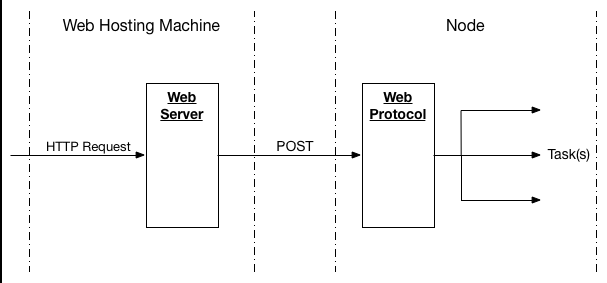
\includegraphics[width=125mm]{images/web_protocol.png}
       \caption{Web Request Translation into Task(s).}
     \end{figure}
     % Support Sentence: Task Translation
     Translation of web requests into tasks, consists of receiving a web request and then the
     web server generates the appropriate RESTful request to be sent to the
     application. For all intent and purposes, any web request is translated into a POST
     request containing the information about the task, such as which module and function
     to call, and the arguments to call it with. Upon receiving the request from the web
     server, the application create a task using the information contained in the request.
     % Support Sentence: Result Returns
     When a task is completed, the result is retrieved by the application deployer node,
     who formulates a HTTP POST request using the web protocol and sends it to the web
     server. The web server then is responsible to present the information back to the
     originator of the initial request.

     % Support Sentence: RESTful API
     The rational behind this, is to completely decouple the presentation logic from the
     application logic, thus maximizing extensibility and modularity. Any web framework
     can be used with this architecture, and it can be hosted on any web service
     provider, as long as it is able to emit/receive HTTP requests it is compatible.
     % Support Sentence: More complex hosting scenarios.
     It is possible to have more elaborate web hosting scenarios, where multiple web
     servers are spun and they all emit HTTP requests to a subset of nodes of an
     application for translation. More meticulous synchronization is required to ensure
     the responses are sent back to the corresponding requesters in that case, but by
     using sessions primitives it is trivial to locate the originating web server, and
     consequently the originator of the request.

     % Concluding Sentence:
     This component is crucial to the claims of extensibility that this architecture
     makes. It is also important in order to achieve scalability for the application
     deployed, where web hosting can be an important bottleneck. Lastly, it provides the
     foundation to implement robust web application, and to provide fault-tolerant
     mechanisms, such as redundant web servers, without incurring any major changes.

     \section{Proof of Concept: Calculator}
     % Topic Sentence:
     In this section we present our very first proof of concept application using this
     architecture. We demonstrate how to create a sensible solution, by reasoning about
     the problem at hand in terms of an Event-Driven Architecture (EDA) and illustrate the
     interaction between the different components. We present the role of each type of
     nodes and their responsibilities and present some conclusions relating to this proof
     of concept.

     % Support Sentence:
     \subsection{Overview}
     The application is a simple web-based calculator. It takes two operands, and
     using a button signifying the operator to be applied, computes the result using the
     resources available to the application (nodes). Four different operators are
     implemented: the addition (+), the subtraction (-), the multiplication (*) and the
     division (/).

     % Support Sentence: Setup
     Implementing this application, we make the following assumptions:
     \begin{itemize}
       \item Web Hosting is the responsibility of the application deployer, thus it will
         host the web server.
       \item No data is persistent, thus we will not require any Data nodes (or database).
       \item No fixed number of Worker nodes. The more nodes available, the more
         concurrent requests can be satisfied.
     \end{itemize}

     % Support Sentence: Web Server
     We have implemented the web server, as mentioned previously, using CherryPy. We present a
     minimalistic web interface that contains 2 fields for each possible operators, 8
     fields in total and 4 buttons, as illustrated in Figure~\ref{calc_home}.
     \begin{figure}[h!]
       \centering
       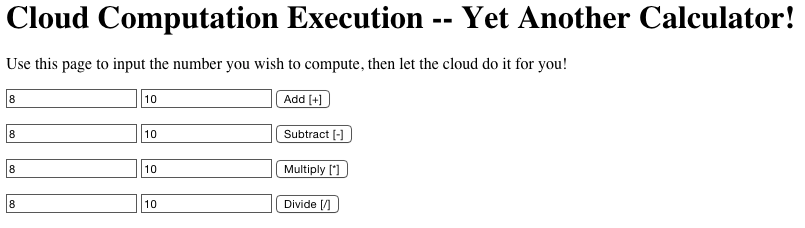
\includegraphics[width=125mm]{images/calc_home.png}
       \caption{Calculator's Web Interface}\label{calc_home}
     \end{figure}

     And the results is presented using a simple string, consisting of: \emph{"The result
       is :"} followed by the result of the computation.

     \subsection{Application Deploying Node}\label{impl_calc_appd}
     % Topic Sentence:
     In this subsection we present the implementation of the Application Deploying Node
     for the Calculator application.

     % Support Sentence: Node Overview
     \begin{figure}[h!]
       \centering
       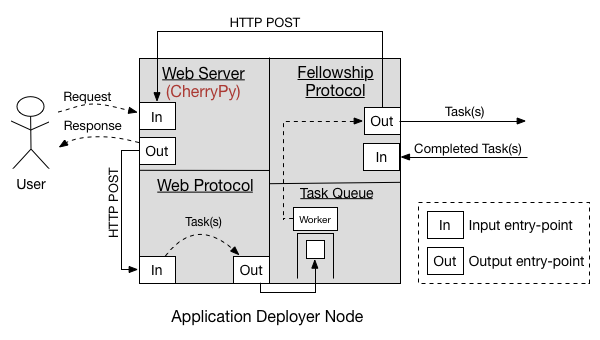
\includegraphics[width=125mm]{images/calc_app_dep.png}
       \caption{Application Deployer Node as part of the Calculator Application.}
     \end{figure}
     As presented in the previous subsection, this node encapsulate the sole event
     generator and event channel of this application. When an event is generated (from the
     web server), it is passed to the event channel (web protocol) where it is translated
     into a task and then queued. Using the Fellowship protocol, this node will dispatch
     the task(s) to the available nodes and collect the result(s) of the completed
     task(s). The results are extracted from the completed task(s), and are presented to
     the end-user as a downstream event-driven activity emerging from the processing of
     the event.

     % Support Sentence: Task queues
     The application deploying node is responsible for the task queues in this specific
     application, because we host the web server on that same node and there are little to
     no value in distributing task queues among several nodes in such a simplistic
     example.

     \subsection{Contributing Node}
     % Topic Sentence:
     In this subsection we present the implementation of a \emph{Contributing Node}, and then
     the logic necessary to process the tasks.

     % Support Sentence: Node Overview
     \begin{figure}[h!]
       \centering
       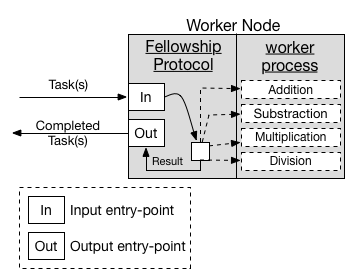
\includegraphics[width=125mm]{images/calc_node.png}
       \caption{Contributing Node as part of the Calculator Application.}
     \end{figure}
     A contributing node receives a task from the application deployer node, executes it,
     and returns the completed task to the application deployer node. All the
     communication between the application deployer node and the contributing node is
     performed using the Fellowship protocol.

     % Support Sentence: worker_process module
     In the context of this application, we have defined the logic to process the various
     tasks into a module called \emph{worker process}. It encapsulates all the logic
     necessary to perform any operation on the two operands, and facilitates the addition
     of new operation, by simply adding a new corresponding function. It makes for a
     clear separation between the application-dependent code and the architecture related
     code, and it augments portability of the source code.

     % Support Sentence: typical task execution
     In order to execute a task, the \emph{contributing node} will call the appropriate
     function inside the module and pass it any parameters necessary using a list of
     parameters. The \emph{contributing node} will append the results to the task object,
     passed in parameters, and reply to the application deployer with the completed task.

     \section{Conclusion}
     We can observe the rudimentary workflow of this architecture: receive a request,
     translate it to task, dispatch the task, execute the task, return the results, and
     respond back to the originator of request. It exemplify the request-response cycle
     perfectly, corresponding to an Event-Driven Architecture.
     \begin{figure}[h!]
       \centering
       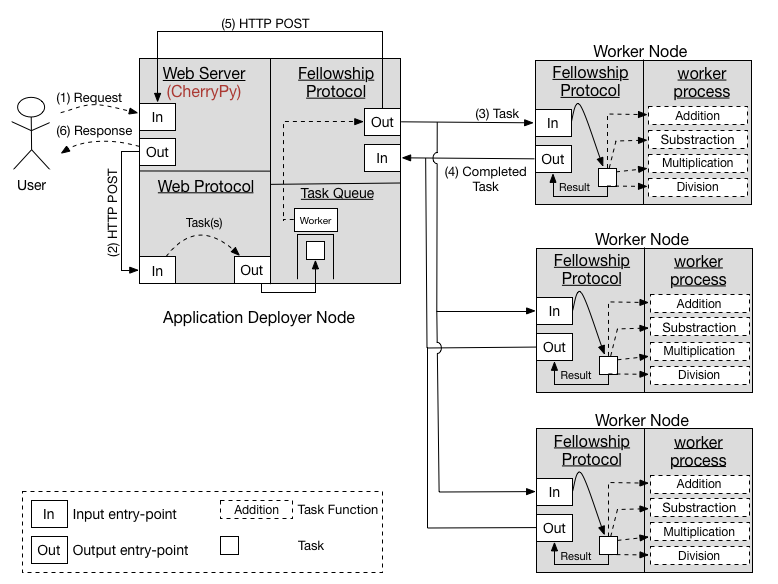
\includegraphics[width=150mm]{images/calculator.png}
       \caption{Calculator Application Architecture Overview.}
     \end{figure}
     Resorting to this way of reasoning is intuitive when developing web-applications. It
     is a central characteristic of this system. This way of reasoning facilitates the
     development of new applications, but also considerably reduces the effort required to
     translate an existing monolithic application into a distributed application, as we
     will see in the following chapter.

     \chapter{Case Study: Multi-Document Text Summarization using Genetic Algorithms}
     \chaptermark{Case Study: MDTS using Genetic Algorithms}
     In the previous chapter, we have introduced the technologies used and the fundamental
     constructs of this architecture. Then, we have presented as a proof of concept, a
     calculator, in terms of our architecture and proceeded to implement it. In this
     chapter, we are presenting an example case study for a more computationally intensive
     application. Namely we present an adaptation\footnote{By no means, is this an
       efficient multi-document text summarization system. But it embodies a
       computationally intensive highly parallelizable problem which is appealing to
       showcase this architecture.} of a system for \emph{Multi-Document Text
       Summarization using Genetic Algorithms} \cite{qazvinian2008summarising}.

     In the following sections, we present the problem at hand and illustrate how a
     genetic algorithm is capable of addressing it. We present how we extend the existing
     work on text summarization using \gls{ga}, in order to process multiple
     documents. We then use an analysis-based approach to translate this problem
     into a distributed web application. This analysis will serve as the foundation to devise
     an algorithm that is compatible with an event driven architecture. Finally, we
     present the characteristics and roles of each type of nodes, and we present a
     discussion of this implementation.

     \section{Problem at Hand}
     % What is Text Summarization?

     In order to provide some context, we present what \emph{Automatic Summarization} is
     in general. Then we present the characteristics of \emph{Multiple-Document Text
       Summarization}, followed by a high-level explanation on how to use \emph{Genetic
       Algorithms} to solve this problem.
     
     This section demonstrates how to transform a monolithic serial program into a
     distributed web-based application, including all the steps required to rationalize
     the transformation. \\

     \emph{Caveat lector:} extensive literature has
     been written on both, Automatic Summarization and Evolutionary Algorithms, and may
     be consulted for more information: see \cite{mani1999advances} as a starting point
     for Automatic Summarization, and see \cite{eiben2008introduction} as an introduction
     to Evolutionary Algorithms.

     \subsection{Automatic Summarization}
     % Topic Sentence:
     To understand how to automate the summarization of documents, we must understand
     what constitutes a summary. A summary can be defined as: the product of a reductive process
     to include salient statements of a source text, by selecting or abstracting the
     original statements, forming a condensed representation of the argumentations and
     conclusions drawn \cite{jones1999automatic}.

     % Support Sentence: What techniques can be used?
     To generate a summary, one of the techniques that can be used relies on the
     \emph{extraction} of linguistic units from a document to represent the information
     conveyed in it. This technique is known as \emph{extraction-based
       summarization}. Another popular technique that can be used to generate a summary,
     consists of \emph{abstracting} the sections from a source text and generate
     statements, using natural language generation techniques, that convey the same
     information in a condensed form. This technique is known as \emph{abstraction-based
       summarization}.

     % Support Sentence: Sentence Extraction (what is it?)
     For this case study, we are interested in extraction-based summarization, more
     specifically we are interested in a technique called \emph{Sentence
       Extraction}. Generally, this technique consists of scoring sentences in a text for
     a set of given metrics, and apply statistical heuristics to filter superfluous or
     not-so relevant sentences.

     % Support Sentence: What if there are multiple document?
     Up until now, we have defined a summary has being derived from a single source text,
     but what if we are presented with a set of documents on a single topic, can we
     summarize the aggregation of all these texts into a single summary? Doing this will
     provide the ability to aggregate all the different perspectives of each text, but
     also to reveal the overlapping perspectives concerning a singular topic. This
     variation of automatic summarization corresponds to \emph{Multi-Document Text
       Summarization (MDTS)} \cite{goldstein2000multi}.


     \subsection{Genetic Algorithms}
     % Support Sentence: Can we do it using GA?
     The problem of creating a summary, using sentence extraction, can be defined as the
     problem of extracting the most salient sentences of a source text, and use them to
     generate a summary of a given length. We can interpret this problem as an
     optimization problem and apply an evolutionary algorithm to search the solution space
     for near-optimal solutions, as proposed by the authors of
     \cite{qazvinian2008summarising} for single document text summarization.

     % Support Sentence: ELIM5 Genetic Algorithm
     A genetic algorithm, is defined as an adaptative heuristic search algorithm inspired
     by biological evolution concepts, such as natural selection, mutations, cross-overs,
     etc. \cite{eiben2008introduction}. A very high-level overview of the outline of a
     simple \gls{ga} is presented in Algorithm~\ref{alg_ga}.
     \begin{algorithm}
     \begin{algorithmic}[1]
     \caption{Genetic Algorithm: An Overview}\label{alg_ga}
     \Procedure{GA}{}
     \BState \emph{Initialize population:}
     \State population = randomPopulation()
     \BState \emph{Evaluate Population:}
     \State fitness = fitnessFunction(population)
     \While{fitness $<=$ desired fitness}
     \State Evaluate Population.
     \State Select parents for next generation.
     \State Perform Crossovers on the parents selected.
     \State Perform Mutations on the resulting population.
     \EndWhile
     \end{algorithmic}
     \end{algorithm}
     There are several considerations to take into account while using \gls{ga}s, especially on
     how to represent an individual in the population, which type of crossovers should be
     applied, enforcing elitism or not in the selection process, the type of mutations to
     apply and how to formulate a meaningful fitness function. But this digression is not
     relevant in the context of this thesis and thus for more information see
     \cite{eiben2008introduction}.

     \subsection{Extensions Proposed for MDTS}
     % Topic sentence:
     We have proposed extensions to the work of \cite{qazvinian2008summarising}, in order
     to provide multi-document summarization capabilities. But first, we present a
     high-level overview of their procedure, and then we present our proposed extensions.

     % Support Sentence: General Workflow
     \begin{algorithm}
     \begin{algorithmic}[1]
     \caption{Automatic Text Summarization using GA: An Overview}\label{alg_ats}
     \Procedure{ATS-GA}{}
     \State Represent document as a Directed Acyclic Graph.
     \State Compute similarity metrics, and weight of the sentences.
     \BState \emph{Initialize population:}
     \State population = randomPopulation()
     \BState \emph{Evaluate Population:}
     \State fitness = fitnessFunction(population)
     \While{fitness $<=$ desired fitness}
     \State Evaluate Population.
     \State Select parents for next generation.
     \State Perform Crossovers on the parents selected.
     \State Perform Mutations on the resulting population.
     \EndWhile
     \State Extract the summary from the graph.
     \end{algorithmic}
     \end{algorithm}

     Algorithm~\ref{alg_ats} is conceptually intuitive. The document is represented using
     a directed acyclic graph to preserve the order of the sentences in the text. In this
     graph, the sentences are the vertices and the similarity between two sentences is
     represented by a directed edge from one sentence to another, where the direction of
     the edge corresponds to the order of the sentences, ensuring a continuous progression
     in the traversal of the graph. The problem then becomes finding a path that traverses
     the graph, containing a number of vertices that corresponds exactly to the desired
     summary length, maximizing the fitness function. Some difficulties can be
     encountered when tuning the parameters of the genetic algorithm, but it is a problem
     inherent to \gls{ga}s in general and not to this specific problem of automatic
     summarization.

     We propose to use this methodology integrally, and execute it in parallel on multiple
     documents sharing a common topic in order to generate a collection of summaries. This
     collection of summaries is then used as a corpus of salient sentences.  Instead of using
     the \gls{ga} to find the final summary, we use a redundancy reduction function to
     remove excessively similar sentences and to achieve the desired summary length. Thus,
     our new and updated algorithm, able to summarize multiple document on a single
     topic is presented in Algorithm~\ref{alg_mdts}.

     \begin{algorithm}
     \begin{algorithmic}[1]
     \caption{Multi-Document Text Summarization using GA: An Overview}\label{alg_mdts}
     \Procedure{MDTS-GA}{}
     \For{\textbf{each} document in collection of documents}
     \State Represent document as a Directed Acyclic Graph.
     \State Compute similarity metrics, and weight of the sentences.
     \BState \emph{Initialize population:}
     \State population = randomPopulation()
     \BState \emph{Evaluate Population:}
     \State fitness = fitnessFunction(population)
     \While{fitness $<=$ desired fitness}
     \State Evaluate Population.
     \State Select parents for next generation.
     \State Perform Crossovers on the parents selected.
     \State Perform Mutations on the resulting population.
     \EndWhile
     \EndFor
     \While{len(summary) $>$ desired summary length}
     \State Apply redundancy reduction algorithm on collection of summaries.
     \EndWhile
     \State Extract the summary from the graph.
     \end{algorithmic}
     \end{algorithm}

     The rational for this extension is the following, given that the genetic algorithms
     finds a near-optimal summary for each document independently then by collecting all
     of these summaries together we have the most salient sentences (in relation to the
     topic) across all documents. Then, we remove the number of less salient sentences for
     which the redundancy score was the highest. The score was computed with respect to
     the number of overlapping words between two sentences, and the closeness to the
     topic.

     \section{Translation of the Problem for this Architecture}
     In this section, we analyze the MDTS system, and translate it into a distributed
     application for our architecture. First, we state the assumptions, then the node
     requirements. Then we identify the logical event flow layers, and present the
     different possible event flows. Finally, we present the resulting workflow of the
     application.\\

     % Support Sentence: Assumptions:
     To start our analysis, we need to make the following assumptions:
     \begin{itemize}
     \item We need to persist (some) data. At least one \emph{Data Node} is required.
     \item We require an arbitrary number of computational resources. At least one
       \emph{Worker Node} is required.
     \item Provide support for multi-tenancy.
     \end{itemize}

     % Support Sentence: Draft out the roster
     Based on the assumptions above we can draft out the node requirements for a minimal
     implementation of this case study: (1) Application Deploying Node, (1) Data Node, and
     (1) Worker Node.

     % Support Sentence: Analyze EDA-Style
     Using these assumptions, we are now capable of analyzing the hypothetical event-driven
     architecture of our application. 

     Appearances might suggest that esoteric rationalizations are required to distinguish
     between an \emph{event} and a \emph{downstream event-driven activity}, we beg to
     differ and suggest this approach and rationale. In this particular case we could
     hypothetically devise two different translations of the problem for this
     architecture: (1) The resulting \gls{eda} contains the sole event generator, the web
     server; and (2) The resulting \gls{eda} contains two event generators, the web server
     and the data node(s). The latter translation distinguishes between a HTTP request
     received from the web server, resulting in a data task to store its content, and the
     worker task created as a result of the completion of the data task. Whereas, the
     former doesn't and rather it proposes to leave these subsequent tasks as part of the
     downstream event-driven activities.
     
     The second possible translation of this problem conflates the definition bestowed
     upon an event in this architecture with a task or self-contained unit of work. In
     this architecture, an event incurs the creation of a series of tasks representing the
     sum total of the work required to account for this event. In the context of web
     applications, we can draw the following analogy between the event and the request
     issued by the end-user: A request is received by the web server and it must formulate
     a response to this request, either by executing a number of operations or retrieving
     information from a data source. In this analogy the fashion in which the response is
     formulated is irrelevant to the end-user, and it can be perceived as a
     \emph{black-box}, similarly for an event from the \gls{eda}'s point of
     view. Everything that happens inside this black-box, as a result from this event, is
     irrelevant in terms of the \gls{eda}. All that matters is that the action(s) taken in
     response to this events yields the desired results, whether this chain of action is
     composed of an arbitrary number of links it is still initiated by an event, and
     ultimately concludes by formulating the appropriate system-response to this event. We can
     now position the concept of downstream \textbf{event-driven} activities as the links
     in the chain of actions undertook to formulate a response to this event, and thus
     these \emph{activities} cannot originate from an event generator.
     
     We can now appreciate why the first possible translation fits naturally within the
     context of this architecture, because an event corresponds to a user request, or the
     initiator of the chain of activities to be performed in order to formulate the
     appropriate system-response to this request, and upon completion no other activities
     are generated for this specific event, marking its termination. In more complex
     examples involving a multi-layered \gls{soa}, it may be justified to further the
     categorization of events with exterior events and interior events for this
     architecture. An exterior event is generated from an event-source that is at the edge
     of the application, i.e., a web server. Whereas an interior event originates from one
     service provider to another inside the \gls{soa}.
     
     As a rule of thumb, one should always try to trace the computational steps of any
     chain of activities and identify its origin. If the originator of the chain of
     activities is a request from the end user, then it is safe to assume that any of the
     subsequent links in this chain are downstream event-driven activities. Conversely, if
     the current step is the originator, and tracing it back would take you outside the
     system, then it is safe to assume that this is an event. Using this approach it is
     trivial to reason about what should be an \emph{event generator}, an \emph{event
       channel}, an \emph{event processing engine} and a \emph{downstream event-driven
       activity}.
     
     % Identify possible: EG, EC, EPG, and DEDA.
     Now, we can identify the logical event flow layers according to our rationalization:
     \begin{itemize}
     \item \textbf{Event Generator(s):} in this case the initial events are generated by
       the web server (incoming request(s) from the user(s)).
     \item \textbf{Event Channel(s):} the web protocol is the event channel.
     \item \textbf{Event Processing Engine(s):} events communicated through the web
       protocol (event channel) are processed by a data node.
     \item \textbf{Downstream Event-Driven Activities:} once a data node completes the
       persistence of the data relative to the user's request, the application logic is
       applied as downstream event-driven activities. This triggers the creation of
       a series of tasks that will carry the execution of the application, involving data
       and worker nodes, and finally returning the result to the web server.
     \end{itemize}
     
     We can distinguish between three event flows from these logical event flow layers:
     (1) \emph{Incoming Request Event Flow}, (2) \emph{Processing a Request Event Flow}
     and (3) \emph{Returning a Response Event Flow}.

     \begin{figure}[h!]
       \centering
       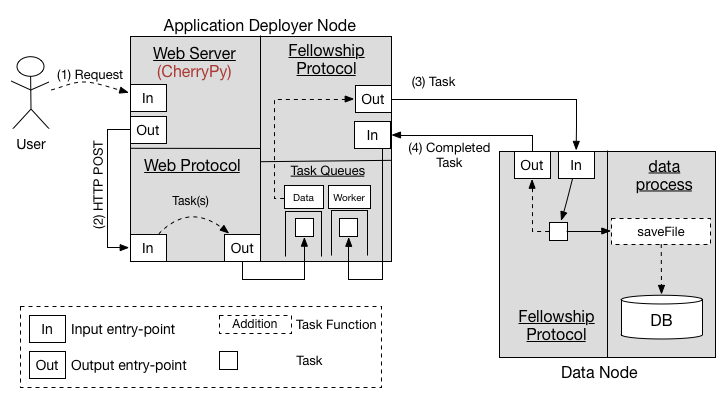
\includegraphics[width=125mm]{images/ef1.png}
       \caption{Event Flow: Incoming Request.}
       \label{ef1}
     \end{figure}

     The \textbf{Incoming Request Event Flow}, as shown in Figure~\ref{ef1}, embodies the
     logic of receiving a request from a user and persisting the data (documents) of this
     request in the database, and queuing up a processing task for this data.

     \begin{figure}[h!]
       \centering
       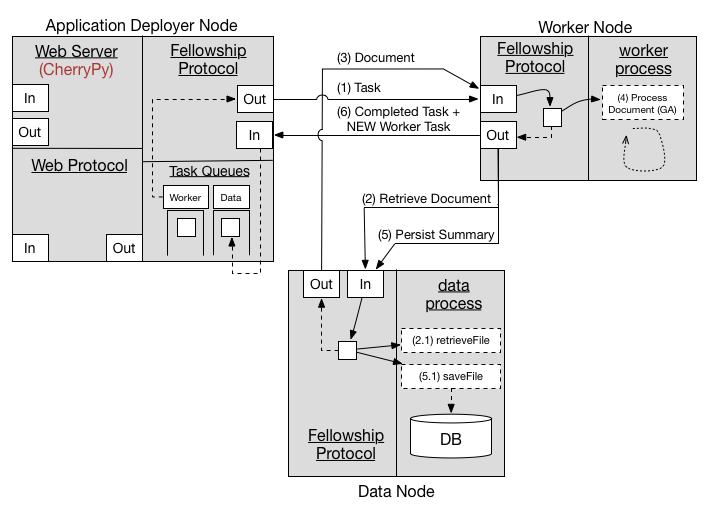
\includegraphics[width=125mm]{images/ef2.png}
       \caption{Event Flow: Processing a Request.}
       \label{ef2}
     \end{figure}

     The \textbf{Processing a Request Event Flow}, as shown in Figure~\ref{ef2},
     corresponds to processing a task related to a document, which implies retrieving the data
     (documents) from the database, processing it using the genetic algorithm, and persisting
     the results back into the database.

     \begin{figure}[h!]
       \centering
       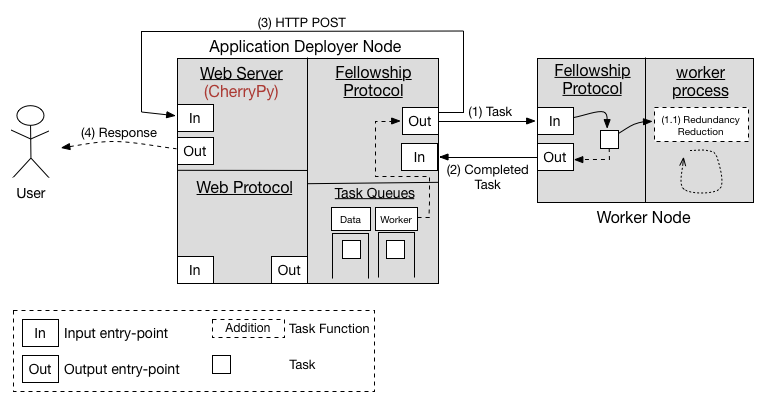
\includegraphics[width=125mm]{images/ef3.png}
       \caption{Event Flow: Returning a Response.}
       \label{ef3}
     \end{figure}

     The \textbf{Returning a Response Event Flow}, as shown in Figure~\ref{ef3}, consists
     of monitoring the database for all the results to be persisted using a database
     trigger\footnote{This is not shown in the figure, the worker task has already been
       created and queued in the figure.} and then creating and dispatching a task to
     process the results by applying the redundancy reduction algorithm. Upon completion
     of the task, the results are sent back to the web server and it presents the results
     to the end-user.

     Based on this analysis we devise a general workflow that encompasses all the
     interactions between the nodes and the end-user concerning a single
     request. Multitenancy is provided through the use of sessions, and we use these
     session primitives to organize the data in the database for each user.

     \begin{figure}[h!]
       \centering
       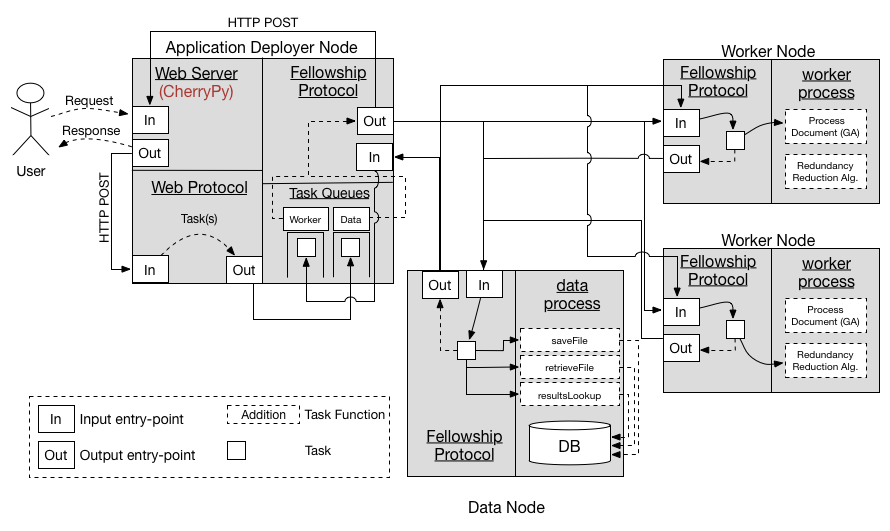
\includegraphics[width=150mm]{images/mdts_overview.png}
       \caption{MDTS: General Workflow.}
     \end{figure}


     \section{Implementation Details}
     % Topic Sentence:
     In this section we present the implementation details for each type of nodes. And we
     outline the specificities of this particular application in the context of our
     architecture.

     \subsection{Application Deploying Node}
     % Support Sentence: Application Deploying Node
     \begin{figure}[h!]
       \centering
       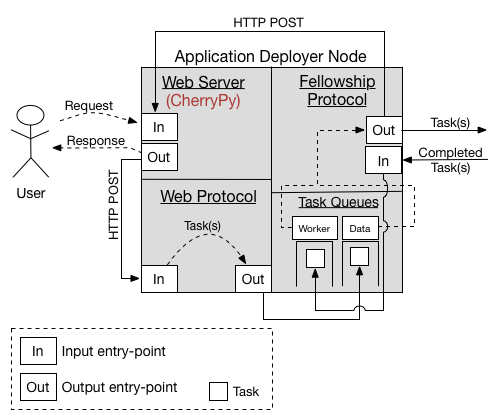
\includegraphics[width=125mm]{images/mdts_app_dep.png}
       \caption{Application Deployer Node as part of the MDTS Application.}
     \end{figure}

     The application deploying node is responsible for receiving the requests from the
     users and translating them into initial data tasks. It is also responsible for the
     task queues, because we host the web server on that same node and there are little to
     no value in distributing task queues among several nodes in this example. Because we
     are using data node(s) we need an additional task queue, thus we have one task queue
     for the worker tasks and one for the data tasks. Thus, the application deploying node
     is responsible for dispatching any tasks contained in its queues, to any
     available nodes.
     % Support Sentence: Data task consequences
     Another characteristic of this implementation of the application deploying node, is
     the task creation logic resulting from a completed data task. As part of the core
     logic of this architecture, when a data task completes the data node can specify a
     post-processing task to be scheduled as the result of this data task. We leverage
     this capability to generate the downstream event-driven chain of activities,
     representing the application logic.
     % Support Sentence: Web Server
     We have implemented the web server, as mentioned previously, using CherryPy. In
     Figure~\ref{mdts_home}, we present a minimalistic web interface, where the users can
     upload their files, specify the different parameters of the genetic algorithm and the
     summarization parameters.

     \begin{figure}[h!]
       \centering
       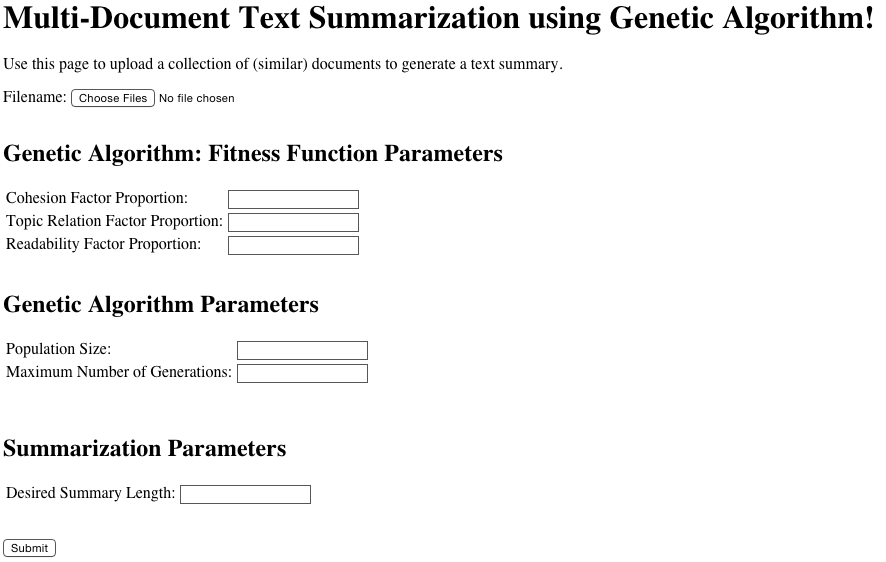
\includegraphics[width=125mm]{images/mdts_home.png}
       \caption{MDTS Application's Web Interface}
       \label{mdts_home}
     \end{figure}

     The results are presented using a simple string, consisting of: \emph{"The result
       is :"} followed by the topic of the documents and the resulting summary.
     % Concluding Sentence:
     There is nothing inherently different between this version of the application
     deploying node and the version presented in the previous chapter, see
     Section~\ref{impl_calc_appd}, aside from the addition of a data task queue. It still
     hosts the web server and it is still responsible for the interactions between the
     contributing nodes and the end-users.

     \subsection{Data Node}
     Data nodes are responsible for persisting the data of the application, which is
     achieved by using a relational database, such as \emph{RethinkDB}
     \cite{rethinkdb}.

     \begin{figure}[h!]
       \centering
       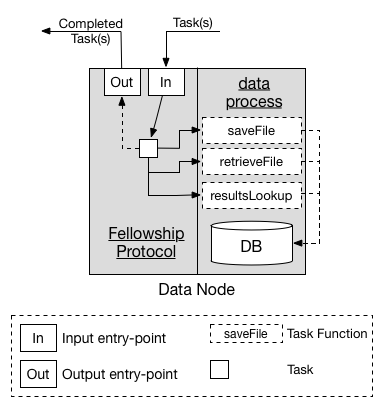
\includegraphics[width=125mm]{images/mdts_data.png}
       \caption{Data Node as part of the MDTS Application.}
     \end{figure}

     % Support Sentence: data_process
     We grouped all of the database functionalities into a single module named
     \emph{dataprocess}, and thus if we would want to replace the implementation of the
     database, only some of the functions need to be redefined in this module. It defines
     a \emph{DataProcess} instance, corresponding to a long-standing process created for
     the database server instance. The \emph{DataProcess} instance contains all the
     information necessary to access the database, such as the client driver port and the
     authentication key. But it also provides the facilities to start and stop the
     database server instance gracefully, through eponymous functions.

     % Support Sentence: Database Schema
     We created a simple database schema, to represent the data that needs to be
     persisted, and we make a distinction between two types of data: \emph{files}, shown
     in Figure~\ref{files_scm}, and \emph{results}, shown in Figure~\ref{results_scm}.

     \begin{figure}[h!]
       \centering
       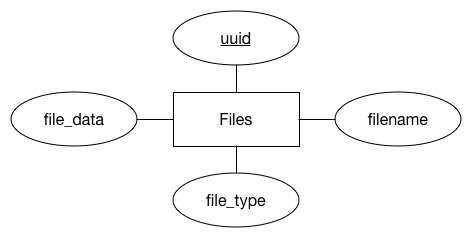
\includegraphics[width=75mm]{images/mdts_files_db_schema.png}
       \caption{Files table schema.}\label{files_scm}
     \end{figure}

     \begin{figure}[h!]
       \centering
       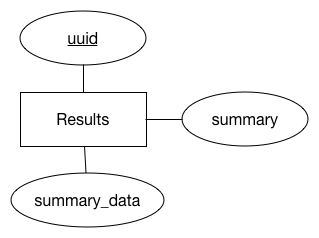
\includegraphics[width=75mm]{images/mdts_results_db_schema.png}
       \caption{Results table schema.}\label{results_scm}
     \end{figure}

     % Support Sentence: Task functionalities
     The task functionalities are implemented in the format defined in
     Section~\ref{impl_constructs_task}, using a list of parameters and passing it
     alongside the task object. We defined three different functions corresponding to the
     actions to perform on the database.

     % Support Sentence: save_file
     The first function is \emph{saveFile}, it consists of extracting a file's content and
     name, from a task object and storing it in the database. Each user has its own
     database, allowing to store very large sets of related documents. If it is the first
     file to be stored, the database and the table corresponding to the \emph{files} table
     schema are created. Upon completion of the task containing the \emph{saveFile}
     function, a \emph{worker} task is created to retrieve the file from the database and
     process it (generate a summary) and to commit the results back to the database.

     % Support Sentence: save_file
     The second function is \emph{retrieveFile} and it consists of retrieving a file from
     the database for a worker node to be processed. The function logic encompasses a
     query to retrieve a file from the appropriate database, the document
     prescribed in the worker task.

     % Support Sentence: results_lookup
     The third function is \emph{resultsLookup} and it consists of creating a trigger that
     monitors the changes in the \emph{results} table. It can be done using the
     primitives offered by \emph{RethinkDB}, such as the \emph{changes()} function, which
     returns a stream of all the changes made to a table or database
     \cite{rethinkdb}. When all the results have been written to the database, the data
     node creates a task indicating that the results are ready to be processed.

     % Support Sentence: Clustering Capabilities
     It is possible to distribute the database across a cluster of data nodes, and we can
     leverage the clustering capabilities of the DBMS to do it. Sharding and Replication
     are automatically taken care of by the DBMS, but can be configured to cater to
     different requirements \cite{rethinkdb}. It is only required to specify the argument
     \emph{--bind all} when starting the instance of the first data node, then any other
     data node can join the cluster by specifying that argument, but also by specifying
     the \emph{--join} argument with the IP address of the first data node. Thus to
     augment the number of data nodes of \textbf{ANY} application, simply specify the
     corresponding arguments when instanciating the data nodes.

     % Concluding Sentence:
     Data nodes are simply database servers, augmented to function within this
     architecture. Their functionalities oscillate around the
     Search-Create-Replace-Update-Delete (SCRUD) operations. Augmenting availability of
     the data can be done effortlessly, on-the-fly by recruiting new nodes and creating
     additional database server instances using the proper arguments.

     \subsection{Worker Node}
     % Topic Sentence:
     Worker nodes are the central components to the business logic of any application
     hosted using this system, because they form the computational resources of the
     system. The re-factoring effort required to transform any function into a task
     function, is minimal.

     \begin{figure}[h!]
       \centering
       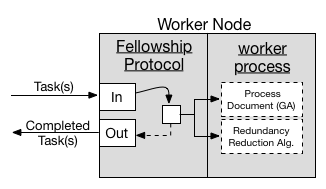
\includegraphics[width=125mm]{images/mdts_worker.png}
       \caption{Worker Node as part of the MDTS Application.}
     \end{figure}

     % Support Sentence: worker_process
     Similarly to the Calculator example, we have encapsulated all the application logic
     into one single module, named \emph{workerprocess}. This module exposes two task
     functionalities\footnote{In all the figures containing a worker node in this case
       study, we changed the task function names to better portray their functionalities
       and thus the function name for \emph{Process Document (GA)} in the module
       corresponds to \emph{retrieveData}. Similarly, the function name for
       \emph{Redundancy Reduction Alg.} in the module corresponds to
       \emph{retrieveDataPostProcessing}.}, again using the format defined in
     Section~\ref{impl_constructs_task}.

     % Support Sentence: retrieveData
     The first function, \emph{retrieveData}, as it name implies is responsible for
     retrieving the data from the database, to create a summary, and to write the results
     back into the database. Our original summarization code required only one
     modification, and it was to tailor the code to process only one document (instead of
     a directory). Ultimately, this function contains the logic to retrieve a document from
     the database, and calls each of the summarization functions in their respective
     order.

     % Support Sentence: retrieve_data_post_processing
     The second function, \emph{retrieveDataPostProcessing}, retrieves the results from
     the database, and applies the redundancy reduction algorithm, then sends the
     resulting summary back to application deploying node to be presented back to the end-user.


     \section{Experimentation}
     In this section, we present the experimental setup used to test and develop the MDTS
     application for this architecture. We conclude with a discussion of our evaluation
     and its limitations.

     Our experimental setup consists of:
     \begin{itemize}
     \item One laptop hosting two \gls{vm}s, where the three are connected using the local
       loopback adapter.
     
       \begin{itemize}
       \item The laptop is an Apple MacBook Pro (15-inch, 2.53GHz, 8GB of RAM, Mid 2009) running OS
         X Yosemite (10.10.2).
       \item We use Oracle VM VirtualBox version 4.3.12 to host the \gls{vm}s on the
         laptop.
       \item Both \gls{vm}s are identical, both were allotted 512MB of base memory, 12Mb
         of video memory, 8 GB SSDs and are running Lubuntu 14.04.

       \end{itemize}
     \end{itemize}

     As per our initial assumptions, we must have at least one application deployer node,
     one woker node, and one data node. The \gls{vm}s corresponds to the contributing
     nodes, and the laptop corresponds to the application deployer node. The contributing
     node's copy of the application differs from the application deployer copy, because
     they are not allowed to instantiate application deploying nodes. The application
     deployer is running a version of this application on MacOS X, whereas the
     contributing nodes are running their applications inside a Docker container. We used
     \textbf{valgrind} instrumentation framework, more precisely \emph{massif}, a tool
     to generate the heap memory profile of applications. We used it to profile the
     application running outside a container, when summarizing 9 documents.
     \begin{figure}[h!]
       \centering
       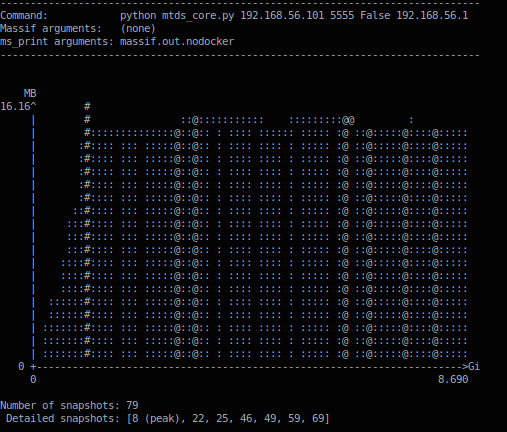
\includegraphics{images/mdts_heap_mem_profile.png}
       \caption{MDTS Application Heap Memory Profile.}\label{profile_mem}
     \end{figure}

     \begin{table}[h!]\label{tbl_profile_mem}
       \begin{tabular}{c*{5}{r}}
         n & time(i) & total(B) & useful-heap(B) & extra-heap(B) & stacks(B)\\
         \hline
         \hline
         0 & 0 & 0 & 0 & 0 & 0\\
         1 & 160,800,345 & 2,789,560 & 2,722,880 & 66,680 & 0 \\
         2 & 319,964,709 & 4,559,048 & 4,464,383 & 94,665 & 0 \\
         3 & 432,207,257 & 4,655,904 & 4,567,228 & 88,676 & 0 \\
         4 & 580,771,287 & 6,908,216 & 6,740,605 & 167,611 & 0 \\
         5 & 711,952,664 & 9,685,952 & 9,479,920 & 206,032 & 0 \\
         6 & 800,083,101 & 10,210,536 & 9,999,586 & 210,950 & 0 \\
         7 & 934,281,944 & 15,176,552 & 14,942,006 & 234,546 & 0 \\
         8 & 1,111,714,521 & 16,942,128 & 16,704,676 & 237,452 & 0 \\
         \hline
       \end{tabular}
       \caption{First 8 Snapshots: Heap Memory Usage Peaking at Snapshot 8.} 
     \end{table}
     Figure~\ref{profile_mem} shows the graphical representation of the memory profile,
     generated using the \emph{ms\_print} tool from the \textbf{valgrind} framework. We
     can observe that this application heap memory profile peaks at 16.94MB, shown in
     Table~\ref{tbl_profile_mem}, and this is used as a baseline to profile the memory
     usage of this application. We say baseline in this context, because it is the
     smallest memory footprint for this application independently of the virtualization
     technology used. Next, we identify how much memory is required to run this
     application inside a container\footnote{Docker was wrote using the emerging Golang
       (or Go) language, and it is not trivial to generate memory profiles for Golang
       binaries because of the immaturity of the language. No tools are available for
       memory profiling, thus we improvise this evaluation scheme, which consists of
       finding the heap memory profile of the \emph{bare} application and add the amount
       of memory used to create and run the container to provide a very high-level
       guesstimation of the actual memory footprint.} using the \emph{free} Unix command
     to capture the amount of memory used before and after the creation of the container,
     shown in Table~\ref{mem_b4} and Table~\ref{mem_after} respectively.

     \begin{table}[h!]\label{mem_b4}
       \begin{tabular}{l*{6}{r}}

         & total & used & free & shared & buffers & cached\\ \hline \hline
         Memory (KB) & 501832 & 481064 & 20768 & 3020 & 76564 & 161628 \\ 
         -/+ buffers/cache (KB) & 242872 & 258960 &&&&\\
         Swap (KB) & 522236 & 348 & 521888 &&&\\
         \hline

       \end{tabular}
       \caption{Memory Statistics Before Container Creation and Execution.}
     \end{table}

     \begin{table}[h!]\label{mem_after}
       \begin{tabular}{l*{6}{r}}

         & total & used & free & shared & buffers & cached\\ \hline \hline
         Memory (KB) & 501832 & 489096 & 12736 & 3180 & 76672 & 162052 \\ 
         -/+ buffers/cache (KB) & 250372 & 251460 &&&&\\
         Swap (KB) & 522236 & 348 & 521888 &&&\\
         \hline

       \end{tabular}

       \caption{Memory Statistics After Container Creation with Active Container.}
     \end{table}
     We can now compute the delta between the memory used before and after, or
     $489096KB - 481064KB = 8032 KB$, then we extrapolate this result, \emph{naively}, to deduce
     that it requires $8032KB$, or around 8MB of RAM to create and execute a idling Docker
     container of Ubuntu 14.04. Thus, our guesstimation of the memory footprint of this
     application running in a Ubuntu 14.04 Docker container is computed by adding the peak
     value of the heap memory profile to the memory required to create and execute the
     container, and is equal to $8032KB + 16942KB = 24974KB$.

     Profiling the application footprint using this improvised scheme has its limitations,
     and we resort to this methodology to provide a glimpse of the \emph{potential} memory
     footprint of this architecture in a real application. Optimizations to the core of
     the architecture framework could definitely be made to augment the performance, and
     effectively reduce the memory footprint. Further experimentations and tests are
     required to provide an accurate memory profile of this architecture. One interesting
     test would remove the use of Docker altogether and resort to the Linux
     containerization primitives directly, then we could profile the memory footprint of
     minimal light virtualization technologies, effectively removing Docker's overhead
     approach our $16942KB$ baseline.

     \section{Conclusions}
     % Recap...
     By reasoning using the event-driven architecture approach, we were able to
     circumscribe any stateful dependencies in the event flows and mitigate them,
     enforcing the task properties of being stateless and persisting data to the
     database. This is a central aspect of this methodology used to translate monolithic
     applications into distributed applications for this system. It also provides the
     tools necessary to divide the application logic into meaningful atomic units of
     work. We have presented a way of dividing an existing application into tasks, but it
     is not the only way to do so. As a matter of fact, a developer has the ability to
     divide the application into many meaningful task, spanning multiple modules, because
     tasks instances are dynamically linked to their functionalities. Thus it is possible
     to use different module names and function names for the functionalities of the
     Worker nodes and the Data nodes.

     All the components of this case study are written using the Python programming
     language. The amount of modifications and coding required to translate this
     application was very small, only 99 additional lines of code to transform the
     summarization logic into worker task functionalities and 164 lines of code for the
     DataProcess class and its (data) task functionalities. The \emph{Web Protocol} was
     written in 113 lines of code, and the web server was written in 145 lines of code.

     The \emph{Fellowship Protocol} is application independent, and is written in 514
     lines of code. Similarly for the core components of this system totalizing 556 lines
     of code, including all the logic pertaining to the nodes and the network interface to
     the \emph{Ring}.

     These numbers include the comments, and it showcases how minimal is the translation
     from a monolithic application to a distributed application, incurring a total of 521
     lines of code for the application-dependent components.

     Using a primitive experimentation environment, we profiled this application with a
     baseline heap memory footprint of $16942KB$ and deduced that \emph{at least} $8MB$ of
     additional memory was required to execute this application in a container. Further
     experimentation is required, and due to the immaturity of the toolset for Golang
     binaries it may be necessary to revert to LxC, or to use directly the
     containerization primitives to gather an accurate memory and performance profile of
     this application, but also of the architecture in general.

     \chapter{Discussion}
     % Topic Sentence:
     In this chapter we present various musings about our architecture and the problems we
     have encountered. We initiate the discussion by presenting the positioning of this
     project amongst the wide landscape of distributed computing platforms. Then conclude
     by presenting various open problems that were encountered along this research path,
     including peer-to-peer networking primitives for collaborative systems, the state of
     the current Internet infrastructure, and ethical problems inherent to public
     collaborative systems.

     \section{Positioning of the System}\label{pos_sys}
     % Topic Sentence:
     In this section we present the positioning of this system amidst the sea of different
     distributed computing platform and systems. It is necessary, because the
     purpose of many of these systems gets conflated together, and it provokes a severe
     misunderstanding of what they provide. This is especially true with cloud computing.

     Cloud computing has become a \emph{buzzword} nowadays, which implies that it becomes
     the go-to solution for all problems. Even today, a majority of professionals are
     still kept in the dark amidst all these promises and features, that very few are
     capable of providing a concise definition of what cloud computing entails
     \cite{cloud_forbes} \cite{cloud_oneil}. We don't blame them. We agree that the
     information circulating around about this technology is, confusing, at best.

     On the other hand, many researchers have tried to devise a proper ontology for this
     \emph{new} paradigm, see \cite{ontology}. This attempt made us realizes that the
     definition of cloud computing can be rationalized, and with the help of documents
     like \cite{nist} it is possible to clearly define cloud computing. But if we attempt
     to complete this already expansive definition, by defining what the end-product of
     cloud computing is, this term \emph{cloud computing} becomes an \emph{umbrella} term
     and can be used to define any distributed system \cite{cloud_citrix} \cite{cloud_tech}.

     Thus, we present this system as being part of a sub-class of cloud computing,
     referred as \emph{volunteer cloud computing}, offering a \gls{paas}-\emph{like} computing
     platform. Notice how we \emph{italicized} the preposition like, we put emphasis on
     the fact that this system is \textbf{not} aimed at providing a volunteer cloud
     computing \gls{paas} service model, but rather a computing platform akin to it. What
     sets them apart, is the environment in which they are intended to operate.

     Our system is meant to operate in a semi-trusted environment, in which the
     contributors (usually) knows (in)directly the application deployers, and thus there
     exist some sort of trust relationship between the two. For example, if we refer to a
     medium to large size secondary school, such an establishment could be the host of
     upwards to 200-300 computers. These computers are used during the day for pedagogical
     purposes, but remains idling or off at night. The school IT administrator, could then
     use this system to provide these 200-300 computers to academics from a local
     university wishing to run scientific experiments. This example prescribes a
     semi-trusted environment, because the academics are in a trust relationship with the
     IT administrator. We qualify this environment as \emph{semi}-trusted, because both
     consumers and producers trust each others, but are required to communicate using
     untrusted networks, such as the Internet.

     Another example, in the context of local communities, could be a chess club, amongst
     any other clubs. Given that the club contains a small community of members, in the
     range of 100-150 members, this system could be used to host their web
     application. Such a web application could contain the statistics about the players,
     recorded games, event announcements, and any other desirable features to chess
     players. Then a subset of the community, at the very least 10 members, could
     contribute their household computing resources to host their web application, and to
     serve their community without incurring any extra cost \footnote{Given that their
       computers are usually turned on, if not then one should factor in the cost of
       electricity.}. Two or three nodes could host the database, to provide
     fault-tolerance in terms of reliability, availability and consistency. Whereas one
     node could host the web server, and delegate two other nodes to take over in case of
     failures, exposing only 3 IP addresses. These nodes are not required to host a
     domain, and could simply connect directly using the IP addresses, but for convenience
     sake's lets assume that they register a domain name to one of these IP addresses. The
     remaining 3-4 nodes can be used as worker nodes, to respond to incoming requests from
     the web server. Again, this is a \emph{semi}-trusted environment because the
     producers and consumers have a pre-existing trust relationship, but operates in a
     public environment. The only cost incurred by this chess club would be the domain
     registration, and it is optional.

     Consequently, we emphasizes that this computing platform caters to a specific niche
     of potential users, but it empowers them to recycle currently available resources and
     to re-factor these resources with a new purpose. All of this, while maintaining a
     focus on providing an intuitive and rational way to reason about how to port such
     applicationss, using event-driven programming model and the Python programming language.

     \section{Problems Encountered}\label{probs}
     % Topic Sentence:
     We have encountered many problems while conducting this research effort, and
     we present the problems that remains open and require further research. \\

     % Overlay networks for collaborative systems
     \\ \textbf{Peer-to-Peer Networking Primitives and Collaborative Systems}\\
     The first problem we have encountered was related to the peer-to-peer networking
     primitives and the collaborative systems, more precisely how well suited are the
     current networking primitives to be used in very-large scale collaborative
     systems. Networking primitive in this context relates to overlay networks connecting
     all the peers in a collaborative system.

     One publication debated this question and the authors of this publication concluded
     that there are no peer-to-peer networking primitive, out of the 12 investigated, that
     caters to all the requirements of a collaborative system \cite{p2p_collab}. We have
     presented these requirements in this thesis in Section ~\ref{rel_EvalFramework}.
     These requirements encompasses the lifecyle of a contributing resource in a
     collaborative system, and present an adequate starting point for the development of
     such systems. Out of the 12 peer-to-peer networking primitives investigated, there
     were 4 unstructured overlay network-based solutions and 8 structured overlay
     network-based solutions. All of these solutions were mutually exclusive with respect
     to their structure and functionalities. The authors are currently working on a
     solution that would account for all their requirements, which has yet to be
     published.

     The major difficulty outlined, was the mutually exclusive characteristics of some
     requirements. Such as the ability to perform deterministic queries and to perform
     \gls{madq}, seems to be completely incompatible because they occur in different
     networking primitives exclusively. Similarly to support mutable object and provide
     the deterministic querying capabilities of structured primitives.  Faced with this
     problem, we decided to create an architecture focused on extensibility, to be able to
     supplant the underlying networking primitive at any desirable point in time, whether
     because a new and more efficient networking primitive has been devised or simply to
     port this system to a different environment.

     Collaborative systems imposes several constraints as a consequence of the environment
     in which these systems operate, but also because of the very collaborative nature of
     these system requiring trust between the participants. We think that this is why this
     problem is difficult, but also why it is interesting. This operating environment is
     paradoxical, because it requires the participants to trust other participants to just
     the right extent, for the it to still be beneficial to offload the workload to the
     participants.

     Consequently, novel peer-to-peer networking primitives are required for this specific
     class of distributing systems, if not to fulfill all the requirements
     \cite{p2p_collab} but to cater to this semi-trusted computing environment, emerging
     out of peer-to-peer collaborative systems.

     \\ \textbf{Collaborative web hosting} \\
     As we already mentioned in Section~\ref{arch_comm}, the current Internet
     infrastructure is not adequate for collaborative web hosting. Furthermore, the
     authors of \cite{ahmed2014collaborative}, present an account of
     these deficiencies and propose a solution to mitigate them.

     They outline the fact that these deficiencies arise from two characteristics inherent
     to peer-to-peer systems. First, is the volatility of the resources and the dynamic
     nature of the networking infrastructure in peer-to-peer system, whereas the current
     Internet infrastructure is stable and \emph{somewhat} static. The second
     characteristic emerges for the constant migration of the data among peers to ensure
     availability and consistency, meaning that one peer may have some data for some time,
     and then it goes offline, it no longer hosts data and it delegates (indirectly) to
     another peer.

     The \emph{naming} scheme employed by the Internet infrastructure is the first
     deficiency presented, it refers to the \gls{dns}. By definition \gls{dns}, operates
     by resolving an IP address from a URL, using a map of URLs and IP addresses. This is
     not adequate in the dynamic environment of peer-to-peer systems, because there are no
     guarantee that the IP address associated with a specific URL corresponds to a live
     node, possibly attempting to access this inaccessible resource.

     The second deficiency presented relates to \emph{searching and indexing} of
     resources. It is traditionally done using a centralized search engine that provides
     the service to locate any resource on the web. Whereas, in peer-to-peer systems
     indexing is (usually) distributed and done on a voluntary basis.

     The last deficiency presented relates to the \emph{content availability}. The current
     web infrastructure relies on web servers to be online continuously.  Whereas in
     peer-to-peer systems, the nodes join and leave the system constantly. It is not easy
     to provide similar availability guarantees using peer-to-peer systems and it is even
     worst in fully decentralized systems. These guarantees are essential for the
     usability of a collaborative web hosting infrastructure.

     This provides a glimpse into the limitations of the current web infrastructure with
     regards to collaborative web hosting, and again for a full and comprehensive account
     followed by a candidate solution please refer to \cite{ahmed2014collaborative}.

     Ultimately, if an application needs to be accessible from the web, it must commit to
     at least one static IP address for the\gls{dns} to include this application as a
     contactable resource on the web. This effectively induce a single point of failure
     into this web-based resource, namely its IP address, exposing the resource to
     potential Denial of Service types of attacks.

     This showcases the immaturity of the Internet as a platform, and how the initial
     design decisions still transpires to this day by exposing the limitation of the
     design.

     \\ \textbf{Ethical use of Computational Resources} \\ The last problem we have
     encountered is a criticism of providing open access to collections computational
     resources.

     One of the underlying factor that drove this research effort, was to explore the
     possibility for the consumer to emancipate itself from current cloud service
     providers and rather, leverage resources from the Internet as a community.
     We were naively inspired by this utopic vision of a computing platform that promotes:
     ecological awareness by recycling rather than consuming new resources,
     censorship-resistance by resorting to decentralized topologies and community by
     sharing \emph{private} resources.

     Upon further investigation, and helpful comments from other researchers we were faced
     with the reality that this vision was in fact utopic, because of which we reposition
     ourselves to preserve our vision but in a more fitting context. We position
     our system to operate in semi-trusted or semi-private environment, which is more
     realistic and provides the liberty to enact our vision. By resorting to whitelisting
     mechanisms we are able to limit access to the this system to only a subset of trusted
     peers. Again, as stated in Section~\ref{pos_sys}, this results in a semi-trusted
     environment, and reduces the risk of malicious nodes harnessing the computational
     resources to commit malicious, even illegal, actions. One example, applicable in a
     untrusted environment without whitelisting mechanisms, is a node that contracts large
     amount of contributing nodes and rather than using these resources to deploy
     legitimate application, this malicious node uses the computational resources to raise
     a bot-net army to perform Distributed Denial-of-Service (DDoS) attacks. 

     Thus, the question raised by this anecdote gravitate around the capacity for the
     ethical use of freely available computational resources in an environment such as the
     Internet. This relates to a field known as \emph{cyberethics}, being highly
     debated in the early days of the Internet, some guidelines were devised such as
     \cite{ethics1989rfc} or \cite{barquin1992pursuit}. The guidelines states that wasting
     computational resources, disrupting the functioning of the Internet, gaining
     unauthorized access to resources, or violating privacy of the users are all deemed
     unethical.

     Now, after quarter-century of continuously presenting similar ethical guidelines to the
     users, it seems that the state of the \emph{open} Internet is more unethical than
     ever. What gives?

     This question is more apt as a philosophy of technology (or information) question,
     and its root cause as well as its potential solutions digresses too much for the scope
     of this thesis. Nonetheless, the implications and consequences of this question are a
     real impeding factor when researching \emph{and} developing Internet related
     technologies. For more information on cyberethics, see \cite{spinello2010cyberethics}
     or \cite{tavani2010ethics}.

     \chapter{Conclusion}
     This thesis presented a distributed computing platform, similar to the \gls{paas}
     computing platform offered by cloud service providers, which is composed of volunteered
     resources rather than dedicated resources. We have illustrated how to provide such a
     platform without introducing any additional resources, but rather by simply recycling
     the resources that are available. As a consequence, the computing platform we have
     proposed is well suited for a variety of devices including lower-end computational
     resources.

     \section{Requirements Fulfilled}
     In the context of this research effort, we focused our attention on two sets of
     requirements simultaneously: (1) The \emph{evaluation requirements}, see
     Section~\ref{rel_EvalFramework}; and (2) The \emph{functional requirements}, see
     Section~\ref{int_req}. The former set of requirements originates from
     \cite{p2p_collab}, and contain the essential phases for a contributing resource in a
     collaborative system. Whereas the latter set of requirements, are the functional
     requirements that we devised for the intended application of this system.

     We consider the five \emph{functional} requirements to be fulfilled as follows:
     \begin{enumerate}[label={\bf Requirement \arabic*},
                       wide=\parindent,
                       leftmargin=\parindent,
                       rightmargin=\parindent]
                     \item Was completely fulfilled by devising the \emph{Ring}
                       abstraction, which provides the means to connect the participants
                       and to manage the application deployment. It effectively supports
                       the deployment of multiple applications simultaneously.
     \item Was fulfilled, because the \gls{api} proposed for the \emph{Application layer}
       does not introduce and/or force any third-party to provide any of the services it
       encompasses. Opting for light virtualization, we enforced the self-containment
       property, not only to the system-level but also to the application-level.
     \item The \emph{security} component of the proposed \gls{api} covers very basic threat
       models common to all web-based applications, including access control,
       authentication and secure communication channels. Also, by choosing a \gls{dht} as
       the networking primitive for the \emph{Ring} abstraction, we obtain a
       decentralized peer-to-peer networking topology.
     \item By design no extra hardware is required, rather it encourages to recycle
       the resources available and enables lower-end and legacy resources to participate. More
       specifically, we reduced the overhead incurred by traditional (full) virtualization
       technologies by using light virtualization technologies, such as containers.
     \item Dynamic membership is designed to be supported by this application, using the
       autonomous \gls{pid} controllers, but still requires to be implemented. We provide
       scalability to the applications hosted using this architecture, through these \gls{pid}
       controllers and because this system is built around asynchronous task queues.
     \end{enumerate}

     We consider to have addressed the \emph{evaluation requirements}, if not
     exhaustively, at least sufficiently to ensure the proper functioning of this system
     as a \emph{collaborative system}. We demonstrate this claim as follows:
     \begin{itemize}
       \item We provide a way to represent resources based on a set of desirable
         attributes, and means to \textbf{Advertise} and \textbf{Discover} these resources
         using the \emph{Ring} abstraction.
       \item We use a two-step best-effort mechanism to \textbf{Select} the most relevant
         resources based on a consumer-defined query using a pub/sub messaging pattern.
         Then, in the second step we provide means to evaluate the inter-resource
         relationships of the tentative selection, effectively addressing the concerns
         expressed in the \textbf{Match} phase.
       \item Using acknowledgments in the \emph{Select} mechanism, we provide this system
         with the ability to \textbf{Bind} the resources to a tentative consumer, thereby
         mitigating any potential concurrent bindings of the same resources to two different
         applications.
       \item Resources are \textbf{Use}d to execute tasks immediately after the
         initialization process is completed.
       \item \textbf{Release} of the resources, is performed autonomously using
         Proportional-Integral-Derivative controllers that continuously monitor the
         workload and performance of each type of nodes in an application, and they
         release any superfluous resources.
     \end{itemize}

     \section{Contributions}
     In this thesis we introduced four contributions which are novel to the best of our
     knowledge, see Section~\ref{contributions}.

     \textbf{Fully-Decentralized Collaborative Web Computing Platform}\\
     Compared to the Cloud@Home system, which provides a full-fledged volunteer cloud
     computing infrastructure and a business-model to entice contributions, we proposed to
     provide a fully-decentralized web computing platform, focusing on the \gls{paas}
     service model. Instead of devising a business model for a completely untrusted
     environment, we resort to a whitelisting mechanism operating in a \emph{semi-trusted}
     environment.

     The Peer-to-Peer Cloud System focuses on a decentralized \gls{iaas} volunteer cloud
     computing infrastructure, whereas our architecture focuses on a decentralized
     \gls{paas} volunteer cloud computing infrastructure operating in a semi-trusted
     environment. Our \gls{api} contains more features than the \gls{api} they offered,
     but doesn't aim to provide the same service model.

     Our platform is decentralized to the extent that is possible within the current
     infrastructure of the Internet. Because it is not possible to associate a URL to a
     non-static IP address, or simply impractical using the current Internet
     infrastructure. Consequently, every Web-based application built for this system will
     have at most one single point of failure, the web server. Thus, unless the
     application is not providing a point of access through the web and resorts to a
     dedicated application communicating directly, this problem remains open.

     The computing platform is flexible enough to cater to a variety of applications, akin
     to what current cloud service providers offer in terms of \gls{paas}. We have
     demonstrated this by implementing two proofs of concept, and have showed how intuitive it
     is to refactor applications for this architecture using the
     event-driven programming model.

     \textbf{Candidate Minimal API Specification for Computing Platforms and/or PaaS}\\
     The \gls{api} devised, see Appendix~\ref{api_appendix}, is based on an investigation of the three major cloud service
     providers: \emph{Google}, \emph{Amazon} and \emph{Microsoft}. It circumscribes the
     essential services and features provided in a computing platform and it is minimal,
     because it provides the basic building blocks for any web applications. Given that a
     \emph{specific} feature is missing, it is easily extensible and can be incorporated into
     the \gls{api}, as long as it is included as an application-specific dependency in the
     container configuration file. Thus, this system provides a computing platform that is
     minimal and does not impose any superfluous features, because it is intended to be
     used with lower-end computing resources. 

     \textbf{Using Light Virtualization to Abstract and Isolate Contributors}\\
     To the best of our knowledge, we are the first to propose the use of \emph{light
       virtualization}, or containers, as an atomic unit composing the computing
     platform and also in the context of \gls{paas}. Since the start of this work,
     the technological landscape shifted and now containers are gaining in popularity,
     especially with the support of major partners like Microsoft.

     \textbf{Minimally Intrusive System Inducing Small Memory Footprint}\\
     Our system is minimally intrusive and intuitive, as shown in the case study of
     \emph{Multi-Document Text Summarization using a Genetic Algorithm}. By resorting to
     \emph{light virtualization} rather than full virtualzation, we have reduced the
     overhead induced by the virtualization technologies to a minimum, while maintaining
     the desirable isolation and abstractive properties of virtualization. However this
     observation is intuitive\footnote{See Section~\ref{fvvslv}.}, and has yet to be
     precisely quantified, but from our early experimentation we have found that the
     memory footprint of the container itself was around $8$MB, which supports our
     intuition.

     \section{Future Work}
     Several research issues were identified while investigating the research problems of
     this thesis. We have identified five short-term research issues that pertain to the
     implementation of this system, and one long-term research issue pertaining to the
     environment of the system. We have presented some open problems that we have
     encountered while writing this thesis, see Section~\ref{probs}, but these problems are
     not specific to our system.\\

     \textbf{Short-term Research Issues}
     \begin{enumerate}
     \item Implement the \emph{T-Man} overlay network gossip-based protocol,
       \cite{jelasity2009t}, to construct the overlay network topologies in the
       \emph{Fellowships}, rather than connecting the nodes directly to each other.
     \item Provide dynamic configuration support for nodes, enabling them to modify their
       configuration at run-time rather than through the modification of configuration
       files.
     \item Implement \gls{pid} controllers to provide dynamic membership capabilities, and
       test how well it operates under various workloads. But also research what kind of
       parameters are suitable for these autonomic controllers, given that in some cases
       it may not be trivial.
     \item Investigate more elaborate access control schemes to evaluate how much change
       is required to adapt this system to an \emph{enterprise} environment, for it to
       operate as an Enterprise Service Bus.
     \item Perform exhaustive performance testing and accurate memory profiling of the
       architecture, in order to identify possible memory leaks and to augment the
       performance of the overall system.
     \end{enumerate}

     \textbf{Long-term Research Issues}\\
     The primary long-term research issue that rises out of this academic inquiry, is how
     can we adapt (if possible) the current system to operate in a fully untrusted
     environment? Researching this issue will enlighten us on how to provide a truly
     public volunteer cloud computing infrastructure using a \emph{decentralized}
     networking primitive. Multiple concerns arises in a fully untrusted environment,
     security being the most obvious one but more precisely how to prevent this system in
     such an environment to be used for malicious intents, such as raising a bot-net army?
     Thus security concerns are supplemented with ethical concerns in an untrusted
     environment, and is it possible to mitigate them using this design?

\begin{appendices}
\chapter{API Specification}\label{api_appendix}

     % ----------------------------------------------------------------------%
     {\small\begin{longtabu} to \textwidth {|X[1 , l ] |X[1 , p ] |}\firsthline\hline
     % -----------------These are headings----------------------------------%
     \textbf{Functions/ Parameters}  & \textbf{Description}  \\ \hline
     %
     \endfirsthead
     %
     \multicolumn{3}{c}%
                 {{\bfseries  Continued from previous page}} \\
                 \hline
                 %
     \textbf{Functions/ Parameters}  & \textbf{Description}  \\ \hline\hline
     \endhead
     %
     \hline \multicolumn{2}{|r|}{{Continued on next page}} \\ \hline
     \endfoot
     %
     \hline
     \multicolumn{2}{|r|}{{Concluded}} \\ \hline
     \endlastfoot
     %-----------Headings end---------------------------------
     \textbf{Database/Storage} & \\
     \hline create(\emph{authKey}) & This function is used to create a database instance
     using a specific authentication key. \\[0.5ex]
     & \textbf{Returns} a new DataProcess instance.\\[0.5ex] \hline
     stop() & This function is used to stop the database server. \\
     & \textbf{Returns} a boolean indicating the outcome of the function.\\[0.5ex] \hline
     start() & This function is used to start the database server. \\
     & \textbf{Returns} a boolean indicating the outcome of the function.\\[0.5ex]\hline
     run(\emph{query}) & This function is used to run a query on the database, sending it
     to the server. \\
     & \textbf{Returns} the result of the query.\\[0.5ex] \hline
     \hline

     \textbf{Network/Communication} & \\
     \hline connect(\emph{node},\emph{list-of-ips}) & This function is used to connect the
     \emph{node}, bootstrapping it to the network using the \emph{list-of-ips}, which
     contains a list of contactable nodes. \\
     & \textbf{Returns} a deferred when this function completes.\\ [0.5ex] \hline
 
    set(\emph{key}, \emph{value}) & This function is used to set a value for a
                                    corresponding key in the \gls{dht}. \\ 
                                    &  \textbf{Returns} a
                                    deferred when this function completes. \\ [0.5ex] \hline

    get(\emph{key}) & This function returns the valued corresponding to the key passed in
                      parameters, if it exists in the \gls{dht}. \\
                      & \textbf{Returns} a deferred with the result.\\ [0.5ex] \hline
    \hline
    \textbf{Load Balancing/Scalability} & \\
    \hline
    workloadWN & Configuration file parameter for the percentage of the desired
    utilization of the \emph{Worker Nodes} \\  [0.5ex] \hline 
    workloadDN & Configuration file parameter for the percentage of the desired
    utilization of the \emph{Data Nodes} \\  [0.5ex] \hline
    coeffP & Configuration file parameter for the coefficient of the P component of the
    PID controller. \\  [0.5ex] \hline
    coeffI & Configuration file parameter for the coefficient of the I component of the
    PID controller. \\  [0.5ex] \hline
    coeffD & Configuration file parameter for the coefficient of the D component of the
    PID controller. \\ [0.5ex] \hline 
    \hline
    \textbf{Security} & \\
    \hline
    checkCredentials(\emph{user}, \emph{hashPW}) & This function takes a username and a hashed password (SHA-2),
                                                   and verifies them against the credentials stored in
                                                   the database. \\
                                                   & \textbf{Returns} a boolean
                                                   indicating whether the credentials are
                                                   verified or not. \\  [0.5ex]
    \hline
    \textbf{Application Deployment/Management} & \\
    \hline
    resourceSpecification & Configuration file parameters for the resource
                            specification to be stored in the \emph{template}. 
                            Example: cpuUsage, memUsage, cpuCapacity, memCapacity,
                            hddCapacity, ... \\  [0.5ex]
    \hline
    \hline
  \end{longtabu}} 

\chapter{Code Samples}
\emph{caveat lector:} this implementation is still in pre-alpha stage, and some details
were left out in order to achieve a working prototype and to produce two proofs of
concepts. It includes, communicating directly between the two processes of the web server
and the Web Protocol, rather than using HTTP POST requests, because these processes were
residing on the same host.

\section{Calculator}
\subsection{Web Server}
\small
\pythonexternal{code_samples/web_calc.py}
\subsection{Web Protocol}
\small
\pythonexternal{code_samples/wP_calc.py}

\section{Multi-Document Text Summarization}
\subsection{Web Server}
\small
\pythonexternal{code_samples/mtds_web.py}
\subsection{Web Protocol}
\small
\pythonexternal{code_samples/wP_mtds.py}
\end{appendices}
\clearpage
\bibliographystyle{alpha} \bibliography{bibliography}

\end{document}
